%Requires the memoir class 
\documentclass[twoside,11pt]{memoir}

%\usepackage{mathptmx}  % Times New Roman, but if you have Garamond 
                        % then use it;
                        % you are writing a book, not a newspaper column

\DoubleSpacing			% memoir's double spacing
\usepackage{rice}		% rice thesis package 
\usepackage[tbtags]{amsmath}	% tbtags argument to make equation number work in split environment.
\usepackage{amssymb, amsfonts}
\usepackage{array}
\usepackage{tabularx}
\usepackage{setspace}
\usepackage{multirow}
\usepackage{rotating}
\usepackage{booktabs}
\usepackage{longtable} % for 'longtable' environment
\usepackage{pdflscape} % for 'landscape' environment
\usepackage{tablefootnote}
\usepackage{mathtools}
\usepackage{physics}
\usepackage{xparse}
\usepackage{adjustbox}
\usepackage{float}
\usepackage{graphicx}
\usepackage[inkscapelatex=false]{svg}
\usepackage[hyperfootnotes=true,
			colorlinks=false]{hyperref}
\usepackage{color}
\usepackage{bm}
\usepackage[]{siunitx}
\usepackage[]{cleveref}
\usepackage[style=phys,
			natbib=true,
			articletitle=true,
			hyperref=true,
			biblabel=brackets,
			chaptertitle=false,
			pageranges=true,
			backend=biber]{biblatex}
\usepackage{csquotes}
\usepackage{caption}
\usepackage{pdfpages}
\usepackage{import}
\usepackage{tikz}
\usepackage{pgfplots}
\usepackage{wasysym}
%\usepackage{subcaption}

% Used for trouble shooting unicode errors. Replaces the unicode character with whatever is in { } so that it's easier to search for in the pdf.
%\DeclareUnicodeCharacter{0301}{!?!}

%%%%%%%%%%%%%%%%%%%%%%%%%%%%%%%%%%%%%%%%%%%%%%%%%%%%%%%%%%%%%%%%%%%
%%%%	Various options
%%%%%%%%%%%%%%%%%%%%%%%%%%%%%%%%%%%%%%%%%%%%%%%%%%%%%%%%%%%%%%%%%%%

% Externalization for pgfplots (https://tex.stackexchange.com/questions/7953/how-to-expand-texs-main-memory-size-pgfplots-memory-overload)
%\usepgfplotslibrary{external}
%\tikzexternalize

\addbibresource{bibliography.bib}

\graphicspath{{chapters/},{appendices/}}

\svgpath{{chapters/},{appendices/}}

% Footnotes are continuously labeled (e.g. without regard for sections, chapters, etc.). 
\usepackage{chngcntr}
\counterwithout{footnote}{chapter}
\interfootnotelinepenalty=10000 %Supposed to keep footnotes from being split

% Additional options
%\sisetup{per-mode=fraction, fraction-function=\flatfrac}
\DeclareSIUnit\Torr{Torr}
\DeclareSIUnit\atoms{atoms}
\DeclareSIUnit\inch{in}
\DeclareSIUnit\gauss{G}

% cleveref options (\Cref{} for start of sentence, \cref{} for abbreviation).
\Crefname{equation}{Equation}{Equations}
\crefname{equation}{Eq.}{Eqs.}
\Crefname{figure}{Figure}{Figures}
\crefname{figure}{Fig.}{Figs.}
\Crefname{table}{Table}{Tables}
\crefname{table}{Tab.}{Tab.}
\Crefname{chapter}{Chapter}{Chapters}
\crefname{chapter}{Ch.}{Ch.}
\Crefname{section}{Section}{Sections}
\crefname{section}{Section}{Section}
\Crefname{appendix}{Appendix}{Appendices}
\crefname{appendix}{Appendix}{Appendices}

% Allows setting l, c, r column widths (needs tabularx)
\newcolumntype{L}[1]{>{\raggedright\arraybackslash}p{#1}}
\newcolumntype{C}[1]{>{\centering\arraybackslash}p{#1}}
\newcolumntype{R}[1]{>{\raggedleft\arraybackslash}p{#1}}

\sisetup{range-units=brackets}

%%%%%%%%%%%%%%%%%%%%%%%%%%%%%%%%%%%%%%%%%%%%%%%%%%%%%%%%%%%%%%%%%%%
%%%%	Definitions
%%%%%%%%%%%%%%%%%%%%%%%%%%%%%%%%%%%%%%%%%%%%%%%%%%%%%%%%%%%%%%%%%%%

% See: https://tex.stackexchange.com/questions/142178/proper-clickable-hyperlinks-with-biblatex-natbib-and-hyperref-author-yea?noredirect=1&lq=1
% thanks to https://tex.stackexchange.com/a/26684/22939
\DeclareCiteCommand{\citejournal}
  {\usebibmacro{prenote}}
  {\usebibmacro{citeindex}%
    \usebibmacro{journal}}
  {\multicitedelim}
  {\usebibmacro{postnote}}

\DeclareCiteCommand{\citebooktitle}
  {\usebibmacro{prenote}}
  {\usebibmacro{citeindex}%
    \usebibmacro{booktitle}}
  {\multicitedelim}
  {\usebibmacro{postnote}}

\DeclareCiteCommand{\citeintitle}% Based on \citetitle from biblatex.def
  {\boolfalse{citetracker}%
   \boolfalse{pagetracker}%
   \usebibmacro{prenote}}
  {\ifciteindex
     {\indexfield{indextitle}}
     {}%
   \iffieldundef{journaltitle}
     {\iffieldundef{booktitle}
        {\iffieldundef{maintitle}
          {\printfield[citetitle]{labeltitle}}% Behave like \citetitle if no "main" title
          {\printtext[maintitle]{\printfield[titlecase]{maintitle}}}}
        {\printtext[booktitle]{\printfield[titlecase]{booktitle}}}}
     {\printtext[journaltitle]{\printfield[titlecase]{journaltitle}}}}
  {\multicitedelim}
  {\usebibmacro{postnote}}


%  Thanks to [Audrey](https://tex.stackexchange.com/a/108349/22939)
\DeclareCiteCommand{\citetitle}
  {\boolfalse{citetracker}%
   \boolfalse{pagetracker}%
   \usebibmacro{prenote}}
  {\ifciteindex
     {\indexfield{indextitle}}
     {}%
   \printtext[bibhyperref]{\printfield[citetitle]{labeltitle}}}
  {\multicitedelim}
  {\usebibmacro{postnote}}


%  Thanks to [Audrey](https://tex.stackexchange.com/a/75916/22939)
  \DeclareCiteCommand{\citeauthor}
  {\boolfalse{citetracker}%
   \boolfalse{pagetracker}%
   \usebibmacro{prenote}}
  {\ifciteindex
     {\indexnames{labelname}}
     {}%
   \printtext[bibhyperref]{\printnames{labelname}}}
  {\multicitedelim}
  {\usebibmacro{postnote}}

%%%%%%%%%%%%%%%%%%%%%%%%%%%%%%%%%%%%%%%%%%%%%%%%%%%%%%%%%%%%%%%%%%%
%%%%	Macros
%%%%%%%%%%%%%%%%%%%%%%%%%%%%%%%%%%%%%%%%%%%%%%%%%%%%%%%%%%%%%%%%%%%

% Inputting pgf image: https://tex.stackexchange.com/questions/127667/matplotlib-pgf-images-in-subdirectory
% Using resizebox: https://tex.stackexchange.com/questions/328281/inserting-and-correctly-scaling-pgf-figure-made-with-matplotlib?rq=1
\newcommand\inputpgf[2]{{
	\let\pgfimageWithoutPath\pgfimage\renewcommand{\pgfimage}[2][]{\pgfimageWithoutPath[##1]{#1/##2}}
	\input{#1/#2}
}}

% Making a command equivalent to \adjustimage but for svg
\newcommand{\adjustsvg}[2]{\adjustbox{#1}{\includesvg{#2}}}

\newcommand{\RomanNumeralCaps}[1]{\MakeUppercase{\romannumeral #1}}

\newcommand{\Sri}{Sr\RomanNumeralCaps{1}}
\newcommand{\Srii}{Sr\RomanNumeralCaps{2}}

\newcommand{\tsup}{\textsuperscript}								% superscript outside math mode.
\newcommand{\tsub}{\textsubscript}									% subscript outside math mode.
\newcommand{\Sr}[1]{\tsup{#1}\text{Sr}}								% ^{8x}Sr outside math mode.
\newcommand{\Srion}[2]{\Sr{#1}\tsup{#2}}							% ^{8x}Sr^{x+} outside math mode.
\newcommand{\Yb}[1]{\tsup{#1}\text{Yb}}								% ^{8x}Yb outside math mode.
\newcommand{\Ybion}[2]{\Yb{#1}\tsup{#2}}							% ^{8x}Yb^{x+} outside math mode.
\newcommand{\Li}[1]{\tsup{#1}{Li}}									% ^{xx}Li outside math mode.
\newcommand{\Rb}[1]{\tsup{#1}{Rb}}									% ^{xx}Rb outside math mode.
\newcommand{\Te}[2]{\tsup{#1}{Te}\tsub{#2}}							% ^{xx}Te_{yy} outside math mode.

\newcommand{\SLJ}[3]{{}^{#1}{#2}_{#3}}
\newcommand{\SLJM}[4]{\SLJ{#1}{#2}{#3}{,\,}{#4}}
\newcommand{\SLJm}[4]{\SLJ{#1}{#2}{#3}{,\,}{m_J = {#4}}}
\newcommand{\SLJF}[4]{\SLJ{#1}{#2}{#3}{,\,}{#4}}
\newcommand{\SLJf}[4]{\SLJ{#1}{#2}{#3}{,\,}{F = {#4}}}
\newcommand{\SLJfM}[5]{\SLJ{#1}{#2}{#3}{,\,}{F = {#4}}{,\,}{#5}}
\newcommand{\SLJfm}[5]{\SLJ{#1}{#2}{#3}{,\,}{F = {#4}}{,\,}{m_F = {#5}}}

\newcommand{\nSLJ}[4]{({#1}){\,}\SLJ{#2}{#3}{#4}}
\newcommand{\nSLJM}[5]{({#1}){\,}\SLJM{#2}{#3}{#4}{#5}}
\newcommand{\nSLJm}[5]{({#1}){\,}\SLJm{#2}{#3}{#4}{#5}}
\newcommand{\nSLJF}[5]{({#1}){\,}\SLJF{#2}{#3}{#4}{#5}}
\newcommand{\nSLJf}[5]{({#1}){\,}\SLJf{#2}{#3}{#4}{#5}}

\newcommand{\nSLJfm}[6]{\nSLJf{#1}{#2}{#3}{#4}{#5}{,\,}{m_F = {#6}}}
\newcommand{\nSLJfM}[6]{\nSLJf{#1}{#2}{#3}{#4}{#5}{,\,}{#6}}
\newcommand{\nSLJFm}[6]{\nSLJF{#1}{#2}{#3}{#4}{#5}{,\,}{m_F = {#6}}}
\newcommand{\nSLJFM}[6]{\nSLJF{#1}{#2}{#3}{#4}{#5}{,\,}{#6}}

\newcommand{\CG}[3]{C^{#3}_{#1;#2}}

\newcommand{\iu}{{i\mkern1mu}}	% i for imaginary unit
\newcommand{\me}{\mathrm{e}}	% e for exponential

% 3j, 6j symbols
\newcommand{\threej}[6]{
	\begin{pmatrix}
		#1 & #2 & #3 \\
		#4 & #5 & #6 
	\end{pmatrix}}

\newcommand{\sixj}[6]{
	\begin{Bmatrix}
		#1 & #2 & #3 \\
		#4 & #5 & #6 
	\end{Bmatrix}}

% Macros for colored lines in captions. Total length = 7mm
\newcommand{\solidrule}[1][1cm]{\rule[0.3ex]{#1}{2pt}}
\newcommand{\solidline}{\mbox{\solidrule[7mm]}}
\newcommand{\dashedline}{\mbox{\solidrule[2mm]\hspace{1mm}\solidrule[2mm]\hspace{1mm}\solidrule[2mm]}}
\newcommand{\dottedline}{\mbox{\solidrule[0.7mm]\hspace{1.4mm}\solidrule[0.7mm]\hspace{1.4mm}\solidrule[0.7mm]\hspace{1.4mm}\solidrule[0.7mm]}}
\newcommand{\dotdashedline}{\mbox{\solidrule[2.25mm]\hspace{1mm}\solidrule[.5mm]\hspace{1mm}\solidrule[2.26mm]}}

%%%%%%%%%%%%%%%%%%%%%%%%%%%%%%%%%%%%%%%%%%%%%%%%%%%%%%%%%%%%%%%%%%%
%%%%	Front-matter details
%%%%%%%%%%%%%%%%%%%%%%%%%%%%%%%%%%%%%%%%%%%%%%%%%%%%%%%%%%%%%%%%%%%

\DoubleSpacing

\begin{document}

\maxtocdepth{subsection}	% put everything into the ToC
\pagestyle{plain}			% pagestyle for the prelims

\frontmatter
\thetitlepage

%%%%	Abstract
\riceabstract
\pagestyle{empty}			% Rice requires no page numbering in the abstract
This dissertation describes the development of an apparatus to undertake spectroscopic studies of \Sr{87} Rydberg states and their application in the production of ultra-long-range Rydberg molecules (ULRRMs). 
Most previous spectroscopic studies of strontium have been performed with the bosonic isotope \Sr{88} which has no nuclear spin ($I = 0$), resulting in a relatively simple and well-understood Rydberg excitation spectrum. 
In contrast, fermionic \Sr{87} has a large nuclear spin ($I = {9}/{2}$) that leads to strong hyperfine interactions which greatly complicate the Rydberg excitation spectrum.
In order to understand the Rydberg states in \Sr{87}, two-photon spectroscopy was performed to measure and identify the $\nSLJ{5sns}{3}{S}{}$ and $\nSLJ{5snd}{3}{D}{}$ hyperfine Rydberg states for $30 \lesssim n \lesssim 99$.
Working with theory collaborators, a detailed understanding of how the hyperfine interaction affects the Rydberg levels is developed and used to extract revised quantum defects.

The detailed understanding of the \Sr{87} hyperfine Rydberg structure was then utilized to produce the first ULRRMs in a fermionic gas.
Unlike traditional molecular binding mechanisms, ULRRMs comprise of one or more ground-state atoms embedded in the electron cloud of a Rydberg atom with the entire system bound together through the weak Rydberg electron-neutral atom scattering. 
Therefore, production of ULRRMs is dependent on both the principal quantum number ($n$) of the parent Rydberg atom and the initial spatial distribution of atoms. 
At low temperatures, the effects of quantum statistics becomes important and result in bunching (bosons) and antibunching (fermions).
These differences in spatial distributions can influence the excitation rates of ULRRMs. 
Current progress in exploring the role of quantum statistics in the excitation of ULRRMs using cold, dense strontium gases is described, with an emphasis on \Sr{87}, and how such measurements can be used to extract the pair correlation function $g^{\pqty*{2}}\pqty*{R}$.
\pagestyle{plain}			% Restore page numbering.

%%%%	Acknowledgments
% put your acknowledgments here 
\riceacknowledgments
\begin{acknowledge}

Acknowledgments go here. 

\end{acknowledge}

%%%%	Dedication
%% \setdedication{ text } % if you want a dedication
%\ricededication

%%%%	Table of contents
%\tableofcontents
\tableofcontents*			% The starred version does not add "Table of Contents" 
							% to the Table of Contents
							% I prefer it this way

% I don't find these two particularly useful
%% \listoffigures			% if you want to include a list of figures  
%% \listoftables			% if you want to include a list of tables

%% if you have more prelim sections, then
%%%% \clearpage
%%%% \pagestyle{plain}
%%%% \prelimtitle   text % for sections after the ToC, etc, before main text

\mainmatter
\pagestyle{rice}

%% Change the spacing between paragraphs, I prefered this for readability 
\let\oldparskip\parskip
\setlength{\parskip}{0.8em}

%%%%%%%%%%%%%%%%%%%%%%%%%%%%%%%%%%%%%%%%%%%%%%%%%%%%%%%%%%%%%%%%%%%
%%%%	Chapters
%%%%%%%%%%%%%%%%%%%%%%%%%%%%%%%%%%%%%%%%%%%%%%%%%%%%%%%%%%%%%%%%%%%

\chapter{Introduction}

***************************************************

*********** NOTES TO SELF, REMOVE LATER ***********

(0) Long-range and anisotropic interactions

(0a) Few-/Many-body physics

(0b) Ultra-long-range Rydberg molecules

(1) Spectroscopy

(2) Effects of quantum statistics -- use Joe's figure?

Add in repumper spectrum.

***************************************************

***************************************************



The ability to produce ultracold samples paved the way towards achievement of quantum degenerate gases of atoms which are ideal systems for studying quantum interactions. 
From the observation of BEC-BCS crossover \cite{Chen2005.PR.412.1, Gurarie2007.JAOP.322.2, Bourdel2004.PRL.93.050401}, superfluid to Mott insulator transition in an optical lattice \cite{Greiner2002.Nature.415.39}, and the formation of matter-wave solitons \cite{Strecker2002.Nature.417.150, Khaykovich2002.Science.296.1290}, most of the work in these systems have been based on a short-range, isotropic contact interactions described by the pseudopotential \cite{Pethick.BEC}
\begin{equation}
	U\pqty{\va{r}}	=	\frac{4 \pi \hbar^2}{m} a_{s} \delta\pqty{\va{r}}
\end{equation}
where $a_{s}$ is the $s$-wave scattering length.
This effective interaction requires the atomic wave functions to overlap. 

An important recent trend in the field of ultracold atomic gases is the study of systems with long-range interactions which can typically be expanded as \cite{Pethick.BEC}
\begin{equation}
	U\pqty{\va{r}}	=	\sum^{\infty}_{k=1} \frac{C_{k} \pqty{\va{r}}}{r^{k}}
\end{equation}
with the ``long-range'' coming from the $U \sim {1}/{r^{k}}$ dependence. 
Depending on the type of interaction (e.g., Coulomb $k = 1$, dipole-dipole $k = 3$, van der Waals $k = 6$), the potentials can be isotropic or anisotropic, providing additional richness to quantum systems and the opportunity to study a wide variety of phenomena including applications towards quantum computing \cite{Jaksch2000.PRL.85.2208, DeMille2002.88.067901}, quantum simulation \cite{deLeseleuc2018.PRL.120.113602, Schauss2018.QST.3.023001}, and tests of theories **** SOURCES? ****
There are several methods for incorporating long-range interactions in to ultracold systems with some of the most prominent being \cite{Lahaye2009.RPP.72.126401}: 
\begin{description}
	\item[Polar molecules]
		These molecules can have large (permanent) electric dipole moments \cite{Aymar2005.JCP.122.204302} and can, ignoring chemical reactions, have extremely long lifetimes. 
		The drawback is that the additional complexity typically makes it very difficult to produce ultracold and quantum degenerate samples. 
		In spite of these challenges, a degenerate Fermi gas of {{\tsup{40}\text{K}}{\tsup{87}\text{Rb}}} was recently achieved by associating atoms from a BEC of {\tsup{87}\text{Rb}} and a degenerate Fermi gas of {\tsup{40}\text{K}} \cite{DeMarco2019.Science.363.853}. 
		Steady progress continues to be made in the direct laser cooling of molecules as well \cite{Anderegg2018.NatPhys.14.890}.
	\item[Magnetic atoms]
		Atoms themselves can have permanent dipole moments which can be exploited to study long-range interactions. 
		Quantum degeneracy has been reached with chromium \cite{Griesmaier2005.PRL.94.160401, Naylor2015.PRA.91.011603}, erbium \cite{Aikawa2012.PRL.108.210401, Aikawa2014.PRL.112.010404}, and dysprosium \cite{Lu2011.PRL.107.190401, Lu2012.PRL.108.215301}.
		Although simpler than molecules, their dipolar interactions are limited by the magnetic moment of atoms and typically requires tuning the short-range interaction strength to be weaker than the dipole-dipole interaction to observe their effects.
		There's also been a recent proposal for creating ultracold dysprosium atoms which exhibit an electric dipole moment in addition to the magnetic dipole moment \cite{Lepers2018.PRL.121.063201}.
	\item[Coupling atoms to a high-finesse cavity]
		An ingenious way of inducing long-range interactions in atomic systems is by placing the atoms in a high-finesse optical cavity such that they couple to the cavity mode which in turn causes the atoms to experience position-based forces \cite{Baumann2010.Nature.464.1301, Mottl2012.Science.336.1570}.
		Although the interactions are (essentially) infinite-range, they are likely to be restricted to only that case. 
		They are also constrained by the geometry of the experiment which could make it difficult to tune between isotropic and anisotropic interactions.
	\item[Rydberg states]
		Highly excited Rydberg states of atoms (and molecules) with principal quantum number $n \gg 1$ can also exhibit strong dipole interactions \cite{Gallagher1994.RydbergAtoms} and have even been observed in solid state systems \cite{Kazimierczuk2014.Nature.514.343}. 
		Since many of the properties of Rydberg atoms scale with $n$, the Rydberg-Rydberg interactions can be tuned in strength and anisotropy by simply exciting different Rydberg states. 
		Rydberg atoms can also leverage well-established techniques for producing quantum degenerate gases of atoms so that their interactions can be readily incorporated to existing setups. 
		The major disadvantage of Rydberg systems are their sensitivities to stray electric fields and the limited Rydberg lifetimes due to both blackbody and Rydberg-Rydberg interactions. 
\end{description}
This thesis will be focused on the latter by studying Rydberg systems in ultracold strontium gases. 
Most ultracold Rydberg experiments have predominantly focused on exciting alkali metal atoms (primarily rubidium and cesium with a growing interest in potassium).
With their hydrogen-like electronic structure, there are well-established methods for both calculating their properties (e.g., see \cite{Sibalic2017.CPC.220.319}) and techniques for producing ultracold and quantum degenerate gases.
But since the interactions are long-ranged, generally comparable to the inter-particle separation in the gas, the particular atomic species used should only affect the details of the interactions but not the overall form. 
As will be discussed below, strontium has some properties which make it a very advantageous system for studying Rydberg physics. 

\section{Rydberg Atoms}

A Rydberg atom can be loosely defined as an atom in an excited state with very large principal quantum number ($n$), i.e., $n \gg 1$. 
Starting in the late {1800's}, it was observed that the wavenumbers of atomic spectra could be described by the formula
\begin{equation}
	\label{eq:Rydberg_formula}
	\nu_{l} = \nu_{\infty,l} - \frac{R}{\pqty{n-\delta_{n,l}}^2}
\end{equation}
where $\nu_{\infty,l}$ is the series limit, $\delta_{n,l}$ is a ``quantum defect'', and $R$ is the Rydberg constant \cite{Rydberg1890.Recherches, Rydberg1890.PM.29.331, Gallagher1994.RydbergAtoms}. 
This is the Rydberg formula.
Conceptually, a Rydberg atom can be thought of as being comprised of a core ion and a highly-excited valence electron which spends the majority of its time far away from the core.
As a result, the Rydberg electron rarely interacts with the core which allows its effects to be characterized by (nearly) constant parameter $\delta_{n,l}$.
While the details of the core ion and electrons are important, which causes $\delta_{n,l}$ to vary from atom-to-atom and from orbital-to-orbital, it generally does not have a large effect on the overall properties of the Rydberg atom.

Although the details of the core are usually small, the principal quantum number does greatly affects the atomic wave function. 
As a result, it sets the energy scale for many interactions which leads to the properties of Rydberg atoms become exaggerated when $n$ becomes large.
\Cref{tab:Rydberg_n-scaling} gives the $n$ dependence for a few Rydberg atoms properties. 
\begin{table}[h]
	\centering
	\caption[]{
		\label{tab:Rydberg_n-scaling}
		Some properties of Rydberg atoms \cite{Gallagher1988.RPP.51.143, Gallagher1994.RydbergAtoms, Camargo2016.PRA.93.022702, Ding2018.PRA.98.042505}.
		*** Double check values!! ***}
	\begin{tabular}{@{}cccc@{}}
		\toprule
		Property					& $n$ scaling	& {Na} : {$\nSLJ{10d}{2}{D}{}$}					& {Sr} : {$\nSLJ{5s38s}{3}{S}{1}$}	\\
		\midrule
		Binding energy				& $n^{-2}$		& $\SI{0.14}{\eV}$								& $\SI{0.01134}{\eV}$				\\
		Coulomb splitting			& $n^{-3}$		& $\SI{0.023}{\eV}$								& $\SI{0.00058}{\eV}$				\\
		Fine structure splitting	& $n^{-3}$		& $\SI{-92}{\MHz}$								& $\SI{2.56659}{\GHz}$				\\
		Orbital radius				& $n^{2}$		& $\SI{147}{\bohr}$								& $\SI{1799}{\bohr}$				\\
		Radiative lifetime			& $n^{3}$		& $\SI{1}{\us}$									& $\SI{21}{\us}$					\\
		Polarizability				& $n^{7}$		& $\SI{0.21}{\MHz\per(\volt\per\cm)\squared}$	& 									\\
		Ionization field			& $n^{??}$		&												& 									\\
		\bottomrule
	\end{tabular}
\end{table}

\subsection{Ultralong-Range Rydberg Molecules (ULRRMs)}

One key aspect to focus on from \cref{tab:Rydberg_n-scaling} is that size of a Rydberg atom increases very quickly with $n$. 
In a dense enough gas, $\ev*{r} \sim n^{2}$ can quickly become comparable to (or larger than) the interparticle separations.
It was in this context, when an atom (or multiple atoms) could be located inside the Rydberg electron's orbit, that a density-dependent shift was first observed in the spectral lines of alkali atoms with the direction of the shift, relative to the unperturbed atomic line, also depended on the buffer gas used \cite{Amaldi1934.NC.11.145, Amaldi1934.Nature.133.141, Liebisch2016.JPB.49.182001, Shaffer2018.NatComm.9.1965}.
\begin{figure}[htbp]
	\centering
	\includegraphics[keepaspectratio, width=\textwidth, height=\textheight]{introduction/rydberg_molecules/orbital_radius-density_n-scaling.pdf}
	\caption[]{
		\label{fig:orbital_radius-density_n-scaling}
		Orbital radius $\ev{r}$ and the corresponding density ${1}/{\ev{r}^3}$ for a strontium Rydberg atom in the $\nSLJ{5sns}{3}{S}{1}$ state.
		The shaded region represents the range of densities typically achievable in ultracold strontium experiments with a maximum of about $\SI{1E15}{\per\cm\cubed}$ occurring in a \Sr{88} BEC \cite{Yan2013.PRL.110.123201, Stellmer2014.arXiv.1307.0601}.}
\end{figure}
\Cref{fig:orbital_radius-density_n-scaling} shows $\ev{r}$ and ${1}/{\ev{r}^3}$ for a strontium atom in the $\nSLJ{5sns}{3}{S}{1}$ state and the typical densities achievable in ultracold gas experiments.
Notice that, even for modest principal quantum numbers and densities, it's easily possible to excite Rydberg atoms much larger than the interparticle separations.

This shift was first explained by Fermi \cite{Fermi1934.NC.11.157}, and later generalized by Omont \cite{Omont1977.JPF.38.1343}, to be the result of low-energy scattering of the Rydberg electron off nearby neutral atoms, formulating the electron-atom interaction with the pseudopotential \cite{DeSalvo2015.PRA.92.031403, Liebisch2016.JPB.49.182001, Shaffer2018.NatComm.9.1965}
\begin{equation}
	V\pqty*{\va{R}}
		=	\sum_{i} \frac{2 \pi \hbar^{2} A_{s}\bqty*{k\pqty*{\va{R}}}}{m_{e}} \delta\pqty*{\va{r}_i - \va{R}}
			+ \frac{6 \pi \hbar^{2} A_{p}^{3}\bqty*{k\pqty*{\va{R}}}}{m_{e}} \overleftarrow{\grad}{\delta\pqty*{\va{r}_i - \va{R}}}\overrightarrow{\grad}
\end{equation}
where $\va{r}_{i}$ is the position of the Rydberg valence electron(s) and $\va{R}$ is the position of the ground-state atom from the Rydberg core. 
On the right hand side, the first term is the $s$-wave contribution and the second term is the $p$-wave contribution with momentum-dependent scattering lengths $A_{s}\pqty{k}$ and $A_{p}\pqty{k}$, respectively, and the semiclassical Rydberg electron momentum given by $\hbar {k \pqty{\va{r}}} = \sqrt{2 m_{e} \bqty{{e^2}/{\pqty{4 \pi \epsilon_0 \va{r}}} - E_{b}}}$ for the unperturbed Rydberg electron binding energy $E_{b}$ \cite{DeSalvo2015.PRA.92.031403}.
Evaluating the interaction with the Rydberg electron wave function $\Psi_{ns}$ leads to \cite{DeSalvo2015.PRA.92.031403}
\begin{equation}
	V\pqty*{\va{R}}
		\simeq	\sum_{i} \frac{2 \pi \hbar^{2} A_{s}\pqty*{k}}{m_{e}} {\abs*{\Psi_{ns}\pqty*{\va{r}_{i} = \va{R}}}^2}
				+ \frac{6 \pi \hbar^{2} A_{p}^{2}\pqty*{k}}{m_{e}} {\abs*{\grad \Psi_{ns}\pqty*{\va{r}_{i} = \va{R}}}^2}
\end{equation}
**** NEED TO DOUBLE CHECK THE ABOVE EQUATIONS ****
A very nice derivation of the interaction is presented in \cite{Bendkowsky2010.PhD}\footnote{She references \cite{Balewski2009.Diploma} which has more details of Fermi's approach.}.

We are particularly interested in the case when, in the low-energy scattering regime, $A_{s} < 0$ because the interaction is attractive and can lead to the formation of bound states nearby ground state atoms in the Rydberg electron wave function.
These are known as ``ultralong-range Rydberg molecules''\footnote{Other objects can also be called ``Rydberg molecules'' (e.g., a molecule electronically excited to a high principal quantum number) but for the purposes of this thesis, a Rydberg molecule refers to the binding of neutral atoms to a Rydberg atom due to scattering.} (ULLRMs) with the binding mechanism, instead of being ionic or covalent, is due to Rydberg-electron neutral scattering and were theoretically predicted by Greene et al., in {2000} \cite{Greene2000.PRL.85.2458}. 
The first experimental detection of ULLRMs occurred in \Rb{87} \cite{Bendkowsky2009.Nature.458.1005} with subsequent observations in {Cs} \cite{Tallant2012.PRL.109.173202} and {Sr} \cite{DeSalvo2015.PRA.92.031403}. 

\Cref{fig:n34_rydberg_molecule_wave_functions_and_spectra} provides an example of the molecular potential and the resulting radial vibration wave functions along with the spectroscopic signal. 
\begin{figure}[htbp]
	\centering
	\includegraphics[keepaspectratio, width=\textwidth, height=\textheight]{introduction/rydberg_molecules/n34-wave_functions_and_spectra/n34-wave_functions_and_spectra.pdf}
	\caption[]{
		\label{fig:n34_rydberg_molecule_wave_functions_and_spectra}
		(Top) Calculated molecular potential ($V$) for a $\nSLJ{5s34s}{3}{S}{1} + \nSLJ{5s^2}{1}{S}{0}$ atom pair together with the radial vibrational wave functions for the $\nu = 0$ to $\nu = 4$ vibrational states.
		(Bottom) Rydberg molecule spectra in unpolarized gas of \Sr{87} and highlighting various dimer vibrational states.}
\end{figure}


****** 

MENTION INTERACION ENERGIES AND NEEDING ULTRACOLD SAMPLES

***********

OFR with Rydberg molecules \cite{Thomas2018.NatComm.9.2238}.

\section{Strontium Rydberg Atoms}

Strontium offer several benefits over the alkali atoms with perhaps the most obvious, as seen in \cref{fig:sr_levels-boson}, being the singlet and triplet Rydberg series due to the two valence electrons.
\begin{figure}[h]
	\centering
	\includesvg[keepaspectratio, width=\textwidth, height=\textheight]{introduction/sr_levels/sr_levels-boson.svg}
	\caption{
		\label{fig:sr_levels-boson}
		Grotrian diagram for (bosonic) strontium (\Sr{88} in particular).
		*** FIX FIGURE -- CHECK SOUMYA'S UPDATED CODE ***.}
\end{figure}
Starting from the $\nSLJ{5s^2}{1}{S}{0}$ ground state, a two-photon excitation can be used to access the myriad of $\SLJ{1}{S}{0}$, $\SLJ{3}{S}{1}$, $\SLJ{1}{D}{2}$, and $\SLJ{3}{D}{1,2,3}$ Rydberg levels.
In addition to the anisotropies of a particular Rydberg orbital, the $C_{6}$ coefficients have been calculated for these states and exhibit both attractive ($C_{6} < 0$) and repulsive ($C_{6} > 0$) interactions \cite{Vaillant2012.JPB.45.135004}. 
The second electron does introduce additional complexity (``richness'') as well due to there being multiple Rydberg series which can interact and typically requires multichannel quantum defect theory (MQDT) \cite{Gallagher1994.RydbergAtoms, Vaillant2014.JPB.47.155001, Robicheaux2018.PRA.97.022508} and/or two-active electron (TAE) models \cite{Ye2013.PRA.88.043430} to described the spectra.
There is also the opportunity to produce doubly-excited and autoionizing states \cite{Gallagher1994.RydbergAtoms} which, besides being interesting in their own right (e.g., \cite{Eichmann1992.PRL.68.21}), have proven to be a sensitive tool for detecting Rydberg atoms \cite{Millen2010.PRL.105.213004, Lochead2013.PRA.87.053409}. 

Another significant advantage of strontium is the narrow $\nSLJ{5s^2}{1}{S}{0} \rightarrow \nSLJ{5s5p}{3}{P}{1}$ transition with linewidth ${\Gamma}/{2 \pi} = \SI{7.5}{\kHz}$. 
Not only does this transition enable us to easily produce samples below about $\SI{2}{\micro\kelvin}$, it is also serves as the first leg of a two-photon transition to a Rydberg state. 
Considering the two-photon coupling between states (in a three-level system) $\Omega \sim {\Gamma}/{\Delta}$ and the photon scattering rate $\Gamma_{\text{sc}} \sim \pqty{{\Gamma}/{\Delta}}^2$ for a detuning $\Delta$ (e.g., see \cite{Metcalf1999.LCT, Bransden.Atoms, Foot2005.Atomic, Steck.QuantumAtomOptics, Gentile1989.PRA.40.5103}), it enables stronger coupling for comparable scattering rates. 
Active research is also progressing towards exciting strontium Rydberg atoms using the even narrower $\nSLJ{5s^2}{1}{S}{0} \rightarrow \nSLJ{5s5p}{3}{P}{0}$ clock transition \cite{Gil2014.PRL.112.103601}. 
In principle, the ultranarrow $\nSLJ{5s^2}{1}{S}{0} \rightarrow \nSLJ{5s5p}{3}{P}{2}$ transition could also be used to excite Rydberg states since a direct measurement of the transition frequency was recently reported \cite{Onishchenko2019.PRA.99.052503}.

A third, more subtle, aspect of strontium is the range of stable isotopes available, both bosonic ($I=0$) and fermionic ($I={9}/{2}$). 
Since all the bosonic isotopes (\Sr{88}, \Sr{86}, and \Sr{84}) have been Bose condensed \cite{Stellmer2009.PRL.103.200401, Martinez2009.PRL.103.200402, Mickelson2010.PRA.81.051601, Stellmer2010.82.041602, Stellmer2013.PRA.87.013611} and a degenerate Fermi gas \Sr{87} has also been produced \cite{DeSalvo2010.PRL.105.030402, Stellmer2013.PRA.87.013611}, strontium provides a unique opportunity for incorporating Rydberg interactions in to both ultracold Bose and Fermi gases (and Bose-Bose and Bose-Fermi mixtures). 
In the bosons, the lack of nuclear spin means there is no hyperfine structure which greatly simplifies the Rydberg spectra whereas the hyperfine structure of \Sr{87} makes the spectra significantly more complicated. 
Overcoming the complexity introduced by the nuclear spin of \Sr{87} provides a unique opportunity for approximating an ultracold classical gas with the atomic population distributed among the $\num{10}$ spin states.

Many of the advantages (and challenges) discussed above for strontium generally apply to other alkaline earth-like atoms (e.g., calcium, barium, ytterbium) as well.






\section{*** MOVE TO EXPERIMENT CHAPTER ***}

***************************************************

*********** MOVE TO EXPERIMENT CHAPTER ***********


Isotope shift of the \SI{461}{\nm} transition.

\begin{table}[h]
	\caption[]{
		\label{tab:blue_isotope_shift}
		Isotope shifts of the $\SI{461}{\nm}$ $\nSLJ{5s^2}{1}{S}{0} \rightarrow \nSLJ{5s5p}{1}{P}{1}$ transition relative to \Sr{88} calculated from the values in \cite{Bushaw2000.SAPB.55.1679}.
		See \cref{tab:blue_isotope_shift_detailed,tab:hyperfine_coefficients_5s5p1P1} for more details.}
	\centering
	\begin{tabular}{@{}cccc@{}}
		\toprule
		Isotope						& Lower level										& Upper level					& $\nu_{A} - \nu_{88}$ [$\si{\MHz}$]	\\
		\midrule	
		\Sr{88}						& $\nSLJ{5s^2}{1}{S}{0}$							& $\nSLJ{5s5p}{1}{P}{1}$		& $\num{0}$								\\
		\midrule	
		\multirow{3}{*}{\Sr{87}}	& \multirow{3}{*}{$\nSLJf{5s^{2}}{1}{S}{0}{9/2}$}	& $\nSLJf{5s5p}{1}{P}{1}{7/2}$	& $\num{-7.8+-0.4}$					\\
									&													& $\nSLJf{5s5p}{1}{P}{1}{11/2}$	& $\num{-49.5+-0.4}$					\\
									&													& $\nSLJf{5s5p}{1}{P}{1}{9/2}$	& $\num{-68.1+-0.4}$					\\
		\midrule	
		\Sr{86}						& $\nSLJ{5s^2}{1}{S}{0}$							& $\nSLJ{5s5p}{1}{P}{1}$		& $\num{-126.3+-0.2}$					\\
		\midrule	
		\Sr{84}						& $\nSLJ{5s^2}{1}{S}{0}$							& $\nSLJ{5s5p}{1}{P}{1}$		& $\num{-273.2+-0.3}$					\\
		\bottomrule
	\end{tabular}
\end{table}

***************************************************

***************************************************
\chapter{Strontium Rydberg experiment}
\label{ch:experiment}

Section intro about the Rydberg experiment.

\section{Vacuum system}

We follow a pretty conventional strontium laser cooling system which uses an oven to produce an atomic beam of strontium which is then slowed by a spin-flip Zeeman slower. 
Similar setups are described in \cite{stellmer2013.phd, barker2016.phd}.
The most noticeable feature is the fact that it was designed to have the center of the main chamber at $\SI{3.5}{\inch}=\SI{8.89}{\cm}$ from the surface of the optical table.
Keeping the working height at this height significantly reduced the need to build a rigid supporting structure to hold the vacuum system above the table as well as the necessary periscopes for the laser beams (although using fibers would mitigate this issue). 
The downside is that it's much more difficult to set up optics below the vacuum chamber, e.g., for the vertical MOT or dipole trap beams. 

Some information about the Rydberg vacuum system can be found in \cite{camargo2015.ms, ding2016.ms}. 

\section{Magnetic field coils}

\subsection{Zeeman slower}

I included information about our Zeeman slower for completeness as Francisco had already made it by the time I joined the experiment so see \cite{camargo2015.ms} for the gory details.

\subsection{Dual MOT coils}

One of the things we did differently from the Neutral experiment is that we have two pairs of MOT coils: the larger pair for the blue MOT and the smaller pair for the red MOT.
This allows us to use two different current supplies without needing a controller which is has the dynamic range to provide the \SI{\sim 40}{\A} to generate the \SI{\sim 40}{\gauss\per\cm} field for the blue MOT while also generating the \SI{\sim 1}{\gauss\per\cm} low-noise field for the red MOT.

\subsection{Trim coils}

The trim coils are used to cancel out stray magnetic fields as well as apply bias fields. 
The two horizontal pairs of rectangular coils are oriented such that the ``X-axis'' produce a field towards or away from the MCP with the ``Y-axis'' perpendicular. 
The ``Z-axis'' coil pair produces a field perpendicular to the table surface. 

Due to the choice of keeping the center of the chamber at \SI{3.5}{\inch} above the table surface, this required the horizontal (X-axis and Y-axis) trim coils to be centered at this height. 

\begin{figure}[htbp]
	\centering
	\includesvg[keepaspectratio=true, width=\textwidth, height=\textheight]{experiment/magnetic_field_coils/trim_coils/trim_coils.svg}
	\caption{\label{fig:trim_coils}Magnetic field trim coils around main chamber. (Blue) X-axis, (green) Y-axis, and (red) Z-axis.}
\end{figure}

The vertical (Z-axis) coils were would on forms around the outside of the top and bottom flanges of the main chamber which allowed us to put many turns on them. 
The circular U-channels used as the forms also feature a radial slice, filled with epoxy, to mitigate the generation of eddy currents. 
In retrospect, we should made the horizontal coils beefier (especially along the X-axis) in order generate larger bias fields along the MCP axis and increase detection efficiency. 
We found that having bias fields along other directions (i.e., not towards/away from the MCP) reduced our detection efficiency, likely due to the Lorentz force steering electrons away from the MCP. 

\section{Laser systems}

\subsection{Versatile blue MOT system}

Section about Zeeman slower and blue cooling setup. Some details about our blue cooling system can be found in \cite{camargo2015.ms, ding2016.ms}. 
After having to send back our Newport TLB-18xx for repairs, we decided to fiber couple the injection path for the Zeeman and MOT slave lasers. 
Fiber coupling allowed us to quickly fix injection lock issues by optimizing the reverse coupling of rejected light from the slave lasers (which counterpropagate the path of the injection light) through the fiber. 

\begin{sidewaysfigure}[htbp]
	\centering
	\includesvg[keepaspectratio=true, width=\paperwidth, height=\paperheight]{experiment/blue_system.svg}
	\caption{\label{fig:blue_system}**Placeholder**Simplified diagram of the blue MOT system.}
\end{sidewaysfigure}

\subsection{Multi-isotope red MOT system}

Some details about our narrow line cooling system can be found in \cite{ding2016.ms}.

\Cref{fig:red_system} shows what the red MOT system looks like when set up for trapping any combination of isotopes. 
In practice, we don't always have all the red MOT AOMs lined up, typically only keeping the AOMs necessary for trapping the isotope(s) for a particular experiment while the other red MOT AOMs are used to generate various other beams (e.g., spectroscopy, ``blow away'', etc.).

\begin{sidewaysfigure}[htbp]
	\centering
	\includesvg[keepaspectratio=true, width=\paperwidth, height=\paperheight]{experiment/red_system.svg}
	\caption{\label{fig:red_system}Simplified diagram of the red MOT system (when everything is put together) for multi-isotope trapping. The master laser frequency is referenced to the $\nSLJ{5s^2}{1}{S}{0} \rightarrow \nSLJ{5s5p}{3}{P}{1}$ in \Sr{88}.}
\end{sidewaysfigure}

Without using a fiber combiner, we're able to devote a lot of power to the red MOT for each isotope, enabling us to use large red MOT beams. 
The drawbacks is that we're much more sensitive to misalignments and the ugly intensity profiles out of the diodes leads to strange red MOT shapes. 

****
Image of \Sr{84} and \Sr{87} red MOTs.
****

\subsection{Optical dipole trap}

Optical dipole traps work by ...... \cite{gri1999.odt}.

Since the $\nSLJ{5s^2}{1}{S}{0}$ electrons are paired, it has a negligible magnetic moment meaning we cannot magnetically trap ground state strontium atoms.
As a result, we use optical traps to confine and evaporatively cool ground state strontium atoms. 

In our setup, we've used both free-space and fibered optical dipole traps but due to having to replace and realign the high-power IR lasers multiple times, we ended up sticking with the fibered systems due to them not losing alignment.
The drawback to the fibered ODT systems is that it's difficult to couple more than about \SI{5}{\W} through continuously without thermal effects degrading the coupling efficiency.
We get around this issue by only having the ODT on at high powers during the transfer from the red MOT before quickly moving in to the evaporation. 

We started with a free-spaced crossed-beam optical dipole trap (XODT) with waists of about $\SI{60}{\um} \times \SI{60}{\um}$. 
This trap was a bit tight but worked well for making \num{100000} BECs of \Sr{84}. 
We found that loading was improved if the trap was artificially widened by driving the AOM with three slightly different frequencies before turning the sideband frequencies down and evaporating \cite{camargo2017.phd}.
After going through three ODT lasers, we stuck with the sheet trap and vertical crossing trap because they were fiber coupled. 


\subsection{A tale of three lasers}

Our first ODT laser was a Coherent Verdi IR - essentially a \SI{1064}{\nm} version of the more common \SI{532}{\nm} variant. 
That worked ok until it died due to an electrical surge (?). 
At which point we moved to using a Nufern NuAmp \SI{50}{\W} fiber amplifier laser.

\section{Making and detecting Rydberg atoms}

\subsection{UV laser system}

This section details the laser system we use to produce \SI{319}{\nm} radiation for two-photon excitation to a Rydberg state. 
Our system for generating the \SI{638}{\nm} radiation is similar to the one described in \cite{mie2014.OE.22.011182}.

Depending on the experiment, whether we want the ability to tune over multiple gigahertz with \SI{\sim 500}{\kHz} linewidth or a laser with a narrower linewidth (\SI{250}{\kHz}), we use either a Koheras Basik BMY10PztSPm or NP Photonics RFLM-50-3-1064.53-1-S-0 ``Rock''. 
The \SI{1064}{\nm} seed is then amplified by an IPG YAR-15K-1064-LP-SF fiber amplifier to about \SI{7.5}{\W}. 

The amplified \SI{1064}{\nm} radiation pumps an Argos (now Lockheed Martin) 2400 CW optical parametric oscillator (OPO) which uses a periodically-poled lithium niobate (PPLN) crystal. 
The crystal first converts $\lambda_\text{pump}=\SI{1064}{\nm}$ to \SI{1.6}{\um} and \SI{3.2}{\um} photons. 
Sum frequency generation then combines a \SI{1064}{\nm} photon with a \SI{1.6}{\um} photon to produce the \SI{638}{\nm} output. 

\begin{figure}[htbp]
	\centering
	\includesvg[keepaspectratio=true, width=\textwidth, height=\textheight]{experiment/uv_system.svg}
	\caption{\label{fig:uv_system}Diagram of the laser system used to produce \SI{318}{\nm} for exciting strontium Rydberg atoms. Diagram of the Argos internals based on the one in \cite{mor2013.RSI.84.013102}.}
\end{figure}

The \SI{7.5}{\W} of \SI{1064}{\nm} gets converted to about **\SI{1.5}{\W}** of \SI{638}{\nm}. 
The Toptica SHG Pro frequency doubles the \SI{638}{\nm} to produce about **\SI{\sim 100}{\mW}** of \SI{319}{\nm} depending how well we optimize the doubling efficiency. 

Depending on the seed we use, we observe linewidths of about **\SI{500}{\kHz} (\SI{< 200}{\kHz})** with the Koheras (Rock).

\begin{align}
	\frac{1}{\SI{1064}{\nm}} &= \frac{1}{\SI{1.6}{\um}} + \frac{1}{\SI{3.2}{\um}} \\
	\frac{1}{\SI{638}{\nm}} &= \frac{1}{\SI{1064}{\nm}} + \frac{1}{\SI{1.6}{\um}}
\end{align}

\subsection{Electric field ionization and detection}

Joe will be detailing the electric field ionization and detection system in his thesis but some details are included here for completeness. 

** picture of the electric field plates and mcp **

Stuff about the scaffold and copper electric field plates. SIMION simulations?

\subsection{Charged particle detection}

Stuff about MCP.

\begin{figure}[htbp]
	\centering
	\includesvg[keepaspectratio=true, width=\textwidth, height=\textheight]{experiment/mcp/mcp.svg}
	\caption{\label{fig:mcp}MCP for detecting charged particles. ** Ceramic spacers were used to help keep the feedthroughs from getting too close. The entire MCP assembly is mounted on a xxxxx feedthrough.**}
\end{figure}

%\chapter{Magic Trap}

Stuff about magic trap.

Wanting to exploit inter- and intra-isotope scattering lengths. 

\section{Preliminary conclusions}

We don't currently have the capability to conclusively determine whether a doubly-degenerate BEC was formed. Blah, blah, blah.
\chapter{Spectroscopy of $\Sr{87}$ Triplet Rydberg States}
\label{ch:fermion_spectroscopy}

As mentioned in \cref{sec:sr_rydberg_atoms}, strontium offers the possibility for exciting ULRRMs in ultracold bosonic, fermionic, and (nearly ideal) classical gases.
In these samples, quantum statistics are expected to affect the excitation rate of ULRRMs where bosonic and fermionic samples are expected to exhibit enhanced and suppressed ULRRM excitation rates, respectively, whereas no change is expected in a classical gas. 
In order to produce ULRRMs, it is necessary to locate and identify the parent Rydberg states. 

An ultracold bosonic gas is represented by \Sr{84} due to the ease of evaporation but, in principle, any of the bosonic isotopes can be used\footnote{An ``ideal'' bosonic gas would better represented by \Sr{88} as $a_{s} \approx 0$ but this isotope difficult to evaporate.}.
Since most spectroscopic studies of strontium Rydberg systems having focused on the most abundant isotope, \Sr{88}, which has no nuclear spin ($I = 0$), there exists a plethora of data available. 
The lack of nuclear spin leads to relatively simple excitation spectra and is relatively well understood \cite{Esherick1977.PRA.15.1920, Beigang1982.OC.42.19, Beigang1982.PS.26.183, Kunze1993.ZPD.27.111, Dai1995.JQSRT.54.1019, Dai1995.PRA.52.4416, Philip2007.OC.279.141, Jackson2018.PhD, Couturier2019.PRA.99.022503}, making it easy to locate \Sr{84} Rydberg states upon appropriate rescaling of the Rydberg constant and using the appropriate ionization limit. 

The fermionic and (approximately) classical ultracold samples are represented by a spin-polarized and unpolarized gas of \Sr{87}, respectively. 
In contrast to \Sr{88}, relatively few studies have been done on \Sr{87}, which has strong hyperfine interactions due to its large $I = {9}/{2}$ nuclear spin. 
It is this hyperfine interaction that significantly complicates the Rydberg excitation spectrum.
Of the previous experimental work \cite{Beigang1981.ZPhys.301.93, Beigang1981.PRL.47.326, Beigang1982.PRL.48.290, Beigang1982.PRA.25.1496, Beigang1983.PRL.51.771}, excitation was performed to singlet $\nSLJ{5sns}{1}{S}{0}$ and $\nSLJ{5snd}{1}{D}{2}$ Rydberg states, with triplet states being observed due to state mixing. 

In order to better understand the \Sr{87} Rydberg series with the goal of producing ULRRMs, we mapped the triplet Rydberg series by directly exciting $\nSLJ{5sns}{3}{S}{1}$ and $\nSLJ{5snd}{3}{D}{1,2,3}$ hyperfine states through the intermediate $\nSLJ{5s5p}{3}{P}{1}$ state. 
To our knowledge, this is the first direct measurement of the \Sr{87} Rydberg states by direct excitation through the $\nSLJ{5s5p}{3}{P}{1}$ state. 

**** ADD A BIT MORE OF A LEAD IN AND OVERVIEW OF CHAPTER? ****

\section{Ionization Limit of $\Sr{87}$}

The first indication that the Rydberg levels of $\Sr{87}$ were not as simple as for the bosonic isotopes was the reported ionization limit, $E_{\text{ion}}^{87} = \SI{45932.2861(10)}{\per\cm}$ \cite{Beigang1982.OC.42.19, Sansonetti2010.JPCRD.39.033103}, being well above those of the bosonic isotopes (see \cref{fig:Eion-mass-scaled} and \cref{tab:ionization_limits}). 
\begin{figure}[htbp]
	\centering
	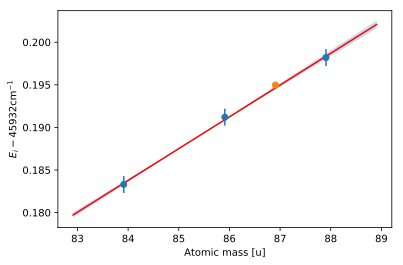
\includegraphics[keepaspectratio, width=4.5in, height=\textheight]{fermion_spectroscopy/calculations/Eion-mass-scaled.pdf}
	\caption{
		\label{fig:Eion-mass-scaled}
		(Blue points) Reported isotopic ionization limits ($E_{\text{ion}}$) vs. isotope mass.
		A linear fit (black line) is used to estimate the $E_{\text{ion}}^{87}$ for an assumed $I=0$ \Sr{87} atom from the ionization energies of the bosonic isotopes. 
		See \cref{ap:sr_data} for isotopic masses and ionization energies.}
\end{figure}
Mass-scaling the ionization energies of the bosonic isotopes suggests that the ionization energy for an assumed $I=0$ \Sr{87} atom should be approximately $\SI{45932.1946+-0.0005}{\per\cm}$, about $\SI{2.74}{\GHz}$ below the reported ionization energy.

The source of this discrepancy is likely related to the hyperfine interaction in the ground state of \Srion{87}{+} since is has a rubidium-like structure with a single valence $s$ electron outside a filled {[Kr]} core.
The hyperfine interaction can be written as (see, e.g., \cite{Steck.QuantumAtomOptics})
\begin{equation}
	\hat{V}_{\text{hf}}	=	A_{\text{hf}} \hat{\va{I}} \vdot \hat{\va{J}}
						=	A_{\text{hf}} \hat{\va{I}} \vdot \hat{\va{S}}
\end{equation}
where $\va{J} = \va{L} + \va{S}$ and $A_{\text{hf}}$ is the strength of the magnetic dipole hyperfine interaction.
Note that there are no higher order contributions (e.g., electric quadrupole) since the valence electron is in an $s$ state so only the contact interaction is non-zero \cite{Arimondo1977.RMP.49.31}.
Following the usual procedure by defining $\va{F} = \va{J} + \va{I}$, the energy shift can be evaluated as
\begin{equation}
	\ev*{\hat{V}_{\text{hf}}}	=	\frac{A_{\text{hf}}}{2} \ev*{\hat{\va{F}}^2 - \hat{\va{J}}^2 - \hat{\va{I}}^2}
								=	\frac{A_{\text{hf}}}{2} \bqty{F \pqty{F + 1} - J \pqty{J + 1} - I \pqty{I + 1}}
\end{equation}
In the ground state of \Srion{87}{+}, $S=s={1}/{2}$ and $I={9}/{2}$ meaning the the $\nSLJ{5s}{2}{S}{1/2}$ is split in to $F = 4$ and $F = 5$ components.
Using $A_{\text{hf}} = \SI{-1000473.673(11)}{\kHz}$\footnote{\citeauthor{Sunaoshi1993.HI.78.241} determined $A_{\text{hf}}$ by measuring the splitting of the $\nSLJf{5s}{2}{S}{1/2}{4}$ and $\nSLJf{5s}{2}{S}{1/2}{5}$ ground state of \Srion{87}{+} in an ion trap. They measured the splitting to be $E_{F=4} - E_{F=5} = \SI{5002368.363(57)}{\kHz}$.} \cite{Sunaoshi1993.HI.78.241}, the $F=4$ and $F=5$ states are shifted by
\begin{equation}
	\ev*{\hat{V}_{\text{hf}}}	=	\begin{cases}
										-\frac{11}{4} A_{\text{hf}} = \SI{2.751302601+-0.000000030}{\GHz}	,{}&{}	F=4	\\
										\frac{9}{4} A_{\text{hf}} = \SI{-2.251065764+-0.000000025}{\GHz}	,{}&{}	F=5
									\end{cases}
\end{equation}
Notice that $\ev*{\hat{V}_{\text{hf}}\pqty*{F=4}} \approx \SI{2.75}{\GHz}$ nearly matches the $\SI{2.74}{\GHz}$ discrepancy between the reported ionization limit of \Sr{87} and the ionization limit determined by mass-scaling from the bosonic isotopes. 
This seems reasonable since most of the earlier spectroscopic work on \Sr{87} primarily focused on the singlet Rydberg states of which converges to the upper $F = 4$ \cite{Beigang1982.PRA.25.1496} state of \Srion{87}{+}. 

% In the analysis below, we used $E_{\text{ion}}^{87} = \SI{45932.1956+-0.0007}{\per\cm}$ for the ionization limit instead of the slightly lower value $E_{\text{ion}}^{87} = \SI{45932.1943+-0.0010}{\per\cm}$ obtained by subtracting $\ev*{\hat{V}_{\text{hfs}}}_{F=4}$ from the reported \Sr{87} ionization limit in \cite{Beigang1982.OC.42.19, Sansonetti2010.JPCRD.39.033103}.
% As described in \cite{Ding2018.PRA.98.042505}, it was found that the higher $E_{\text{ion}}^{87}$ resulted in the quantum defects of the $\nSLJ{5sns}{1}{S}{0}$ and $\nSLJ{5sns}{3}{S}{1}$ states converging to a nearly constant value.

\section{Publication: Spectroscopy of \Sr{87} Triplet Rydberg States}

Below is a reproduction of our work, published in \cite{Ding2018.PRA.98.042505}, which was a combined experimental and theoretical study of $\nSLJ{5sns}{3}{S}{1}$ and $\nSLJ{5snd}{3}{D}{1,2,3}$ Rydberg states in \Sr{87}.
The experimental work was undertaken at Rice University with theory collaborates at the Institute for Theoretical Physics, Vienna University of Technology. 
R.D., J.D.W., and S.K.K. took the experimental data. R.D. compiled and analyzed the data. S.Y. developed the theoretical framework for \Sr{87} and performed the calculations. 
The paper was written collaboratively between R.D., S.Y., and F.B.D. S.Y. wrote the theoretical section and performed extracted the quantum defects from the \Sr{87} data. R.D. wrote the experimental section and compiled the data tables. S.Y. and F.B.D. wrote the introduction, results, and conclusion sections.

\begin{center}
	Phys. Rev. A \textbf{98}, 042505 (2018)
	
	R. Ding, J. D. Whalen, S. K. Kanungo, T. C. Killian, and F. B. Dunning	\\
	\textit{Department of Physics and Astronomy, Rice University, Houston, Texas 77005, USA}

	S. Yoshida and J. Burgd{\"{o}}rfer	\\
	\textit{Institute for Theoretical Physics, Vienna University of Technology, A-1040 Vienna, Austria, European Union}
\end{center}

\subsection{Abstract}

A combined experimental and theoretical spectroscopic study of high-$n$, $30 \lesssim n \lesssim 100$, triplet $\SLJ{}{S}{}$ and $\SLJ{}{D}{}$ Rydberg states in \Sr{87} is presented. 
\Sr{87} has a large nuclear spin $I = {9}/{2}$, and at high-$n$ the hyperfine interaction becomes comparable to, or even larger than, the fine structure and singlet-triplet splittings, which poses a considerable challenge both for precision spectroscopy and for theory.
For high-$n$ $\SLJ{}{S}{}$ states, the hyperfine shifts are evaluated nonperturbatively, taking advantage of earlier spectroscopic data for the $I = 0$ isotope \Sr{88}, which results in good agreement with the present measurements. 
For the $\SLJ{}{D}{}$ states, this procedure is reversed by first extracting from the present \Sr{87} measurements the energies of the $\SLJ{3}{D}{1,2,3}$ states to be expected for isotopes without hyperfine structure (\Sr{88}), which allows the determination of corrected quantum defects in the high-$n$ limit.

\subsection{Introduction}
\label{S:into}

Rydberg excitation in dense cold-atom samples can lead to the formation of ultralong-range Rydberg molecules in which scattering of the Rydberg electron from neighboring ground-state atoms leads to the binding of one or more ground-state atoms in multiple possible vibrational levels \cite{Greene2000.PRL.85.2458, Bendkowsky2009.Nature.458.1005, Li2011.Science.334.1110, Tallant2012.PRL.109.173202, DeSalvo2015.PRA.92.031403, Bellos2013.PRL.111.053001, Sassmannshausen2015.PRL.114.133201, Krupp2014.PRL.112.143008, Anderson2014.PRL.112.163201, Booth2015.Science.348.99, Eiles2015.PRL.115.193201, Eiles2017.PRA.95.052708, Gaj2014.NatComm.5.4546, Dunning2016.JPB.49.112003}
Measurements of such weakly bound Rydberg molecules have also been extended to dense Bose-Einstein condensates (BECs) and higher-$n$ values where the Rydberg electron orbit can enclose tens to hundreds of ground-state atoms \cite{Butscher2011.JPB.44.184004, Camargo2018.PRL.120.083401, Kleinbach2018.PRL.120.193401}.

The interaction between the excited Rydberg electron and a ground-state atom can be described using a Fermi pseudopotential. 
For strontium, except at short ranges, $s$-wave scattering dominates due to the lack of a $p$-wave resonance. 
This results in an oscillating molecular potential that reflects the modulations in the electron probability density \cite{Bendkowsky2009.Nature.458.1005}. 
The largest, and deepest, potential well is located near the outer classical turning point and the wave function of the ground vibrational state of the Rydberg molecule is strongly localized in this region. 
Thus, the probability for forming a ground-state dimer molecule will depend on the likelihood of initially finding a pair of ground-state atoms at the appropriate internuclear separation $R$. 
By varying $n$ and the location of the potential minimum, one can probe the pair correlation function in the ultracold gas. 
This provides an opportunity to examine the influence of quantum statistical properties on Rydberg molecule formation. 
Strontium is an attractive candidate for such a study because it possesses both bosonic (\Sr{84}, \Sr{86}, and \Sr{88}) and fermionic (\Sr{87}) isotopes, all of which have been cooled to degeneracy. 
The excitation spectra for the bosonic isotopes are particularly simple as they have zero nuclear spin ($I = 0$) and therefore no hyperfine structure. 
In contrast, \Sr{87} has nuclear spin $I = {9}/{2}$, which results in hyperfine interactions that greatly complicate the excitation spectrum.  

Several studies of Rydberg spectra for bosonic \Sr{88} have been reported \cite{Vaillant2012.JPB.45.135004, Esherick1977.PRA.15.1920, Beigang1982.PS.26.183}. 
These studies primarily centered on lower-$n$ states ($n \lesssim 40$) and focused on the perturbations introduced by channel interactions and their treatment using multichannel quantum-defect theory (MQDT). 
Information on higher-$n$ levels was typically obtained by extrapolating the measured quantum defects using the Rydberg-Ritz formula. 
Such extrapolation is known to be an effective method for predicting the energies of high-$n$ Rydberg states whose quantum defects are essentially $n$ independent and therefore nearly constant. 
This, however, is not true for strontium $\SLJ{}{D}{}$ states whose quantum defects exhibit a relatively strong $n$ dependence. 

Experimental and theoretical studies of the spectrum for \Sr{87} have also been reported \cite{Beigang1981.PRL.47.326, Beigang1982.PRL.48.290, Beigang1982.PRA.25.1496, Beigang1983.PRL.51.771, Beigang1988.JOSAB.5.2423, Sun1989.JPB.22.2887}. 
These include measurements at low $n$, where the hyperfine interaction can be treated as a weak perturbation, and at high $n$ ($n \sim 100$), where the hyperfine shift becomes comparable to or even larger than the energy spacing between adjacent unperturbed states. 
Analysis of the high-$n$ spectrum therefore poses a considerable challenge and requires use of nonperturbative methods. 
One possible approach is to take advantage of the accurate spectral information available for the bosonic isotope \Sr{88} and use it to estimate the spectrum for \Sr{87} \cite{Beigang1981.PRL.47.326, Beigang1982.PRL.48.290, Beigang1982.PRA.25.1496, Beigang1983.PRL.51.771}. 
For $\SLJ{}{S}{}$ states this approach provides energy levels that agree reasonably well with measured data \cite{Beigang1981.PRL.47.326, Beigang1982.PRL.48.290, Beigang1982.PRA.25.1496, Beigang1983.PRL.51.771}. 
A similar method utilizing a truncated basis set has been used to study low-$n$ ($n < 20$) \Sr{87} $\SLJ{}{D}{}$ states \cite{Beigang1982.JPB.15.L201}. 

However, the high-$n$ levels were analyzed by MQDT \cite{Sun1989.JPB.22.2887} because no corresponding measured levels for the bosonic isotopes were available. 
Earlier spectroscopic studies utilized a heat pipe, which can introduce uncertainties due to Doppler and pressure broadening. 
Moreover, Stark shifts due to the presence of stray fields could not be controlled. 
Indeed, for high-$n$ states, $n \gtrsim 100$, additional \textit{ad hoc} corrections were introduced to obtain agreement between the theoretical estimates and the experimental measurements. 

In this work we measure and analyze the excitation spectrum for high-$n$ ($50\lesssim n \lesssim 100$) $\SLJ{}{S}{}$ and $\SLJ{}{D}{}$ Rydberg states created in an \Sr{87} ultracold gas using two-photon excitation as a precursor to planned studies of Rydberg molecule formation in fermionic gases. 
Measurements using ultracold atoms are expected to be more accurate than measurements in a heat pipe because Doppler and pressure broadening are well suppressed and stray fields can also be controlled. 
In the present two-photon excitation scheme the intermediate $\nSLJ{5s5p}{3}{P}{1}$ state is used instead of the $\nSLJ{5s5p}{1}{P}{1}$ state employed in earlier studies. 
Since the $\nSLJ{5s5p}{3}{P}{1}$ state has a much longer lifetime than the $\nSLJ{5s5p}{1}{P}{1}$ state ($\tau = \SI{21}{\us}$ and $\tau = \SI{5}{\ns}$, respectively), broadening induced by scattering off the intermediate state is also suppressed. 

We compare our experimental data with predictions derived from a semiempirical theoretical description that exploits spectroscopic data for the bosonic isotopes. 
This approach produces satisfactory agreement with the present measurements. 
We also derive improved Rydberg-Ritz formulas for both $\SLJ{}{S}{}$ and $\SLJ{}{D}{}$ states at very high $n$. 

\subsection{Theoretical Approach}
\label{S:Theoretical approach}

An \textit{ab initio} theoretical description of the electronic structure of strontium Rydberg atoms with a precision of $\SI{\sim 10}{\MHz}$ or better is currently out of reach. 
Thus, in order to arrive at a quantitative and predictive description, it is necessary to resort to semiempirical methods. 
The theoretical approach adopted here follows that of earlier work by Beigang and co-workers \cite{Beigang1982.PRA.25.1496, Beigang1983.PRL.51.771}.

The underlying idea is to exploit the much simpler (and for $\SLJ{}{S}{}$ states, better known) electronic structure of the bosonic isotope \Sr{88} as reference for \Sr{87} to accurately account for the perturbations introduced by hyperfine interactions by direct diagonalization. 
The spectroscopic data for \Sr{88} thus serve as an analog simulation of the full $N$-electron Schr{\"o}dinger equation that accounts for electron correlation and configuration interactions, which are tacitly assumed to be the same for all the isotopes. 
Isotope-specific interactions are then taken into account nonperturbatively by diagonalizing the full Hamiltonian which includes the hyperfine interaction. 
Accordingly, the Hamiltonian $H(87)$ for \Sr{87} is written as
\begin{equation}
	\label{eq:hamil}
	H(87)	=	H_0(88,m_{87}) + V_{\text{hf}}	,
\end{equation}
where $H_{0}(88,m_{87})$ plays the role of the unperturbed Hamiltonian that yields the eigenstates and eigenenergies, i.e., spectral lines, for \Sr{88} but rescaled by the isotope shift corresponding to the reduced mass $m_{87} = m_e M_{87}/{(m_e + M_{87})}$, where $m_e$ is the electron mass, $M_{87}$ is the mass of {\Sr{87}\tsup{+}} ion, and $V_{\text{hf}}$ is the hyperfine interaction. 
Corrections beyond the elementary isotope shift, in particular, the mass polarization correction, can be estimated from earlier data for helium Rydberg states \cite{Cok1979.PRA.19.1830, Cok1981.PRA.24.3283, Veldt1990.PRA.41.4099} and, upon rescaling to {Sr}, are found to be $\SI[input-comparators=\lesssim]{\lesssim 1}{\MHz}$ and can therefore be neglected. 

The Hamiltonian ${H(87)}$ [\cref{eq:hamil}] is diagonalized using the basis states $\ket*{[(5sn\ell) \, ^{2S+1}L_J, I] F}$ constructed by the coupling of angular momenta $\va{F} = \va{J} + \va{I}$, where $\va{I}$ is the nuclear spin and $\ket*{(5sn\ell) \, ^{2S+1}L_J}$ are the eigenstates of $H_{0}(88,m_{87})$. 
We note that we retain the conventional Russell-Saunders ${}^{2S+1}L_J$ notation for the eigenstates of $H_0(88,m_{87})$ even though $S$ and $L$ are not exactly conserved quantum numbers in the presence of the spin-orbit interaction. 
In this basis $H_0(88,m_{87})$ is diagonal with corresponding eigenenergies
\begin{equation}
	\label{eq:ene0}
	E_{n,S,L,J}^{(0)} = E_{\text{ion}}^{(0)} - \frac{R(m_{87})}{(n - \mu^{(0)}_{n,S,L,J})^2}	,
\end{equation}
where $E_{\text{ion}}^{(0)}$ is the energy corresponding to the first ionization threshold of \Sr{87} assuming $I = 0$, $\mu^{(0)}_{n,S,L,J}$ is the quantum defect for the state $\ket*{(5sn\ell) \, ^{2S+1}L_J}$, and ${R(m_{87}) = R_{\infty} m_{87} / m_e}$ with the Rydberg constant $R_{\infty}$. 
In the following we use either directly measured or extrapolated (at high-$n$) quantum defects for \Sr{88} as input.

The hyperfine interaction results from the interaction between an electron and the electric and magnetic multipoles of the nucleus \cite{Schwartz1955.PR.97.380}. 
For singly excited high-$n$ strontium atoms with two electrons outside closed shells, $V_{\text{hf}}$ is governed by the interaction of the $5s$ valence and $n\ell$ Rydberg electrons with the \Sr{87} nuclear spin $I = {9}/{2}$. 
Because of the ${(n^{*})}^{-3}$ scaling of the hyperfine interaction \cite{Gudde1993.PRA.47.4725}, the hyperfine shift associated with the Rydberg electron for {high-$n$} values (${n > 20}$) can be estimated to be $\SI[input-comparators=\lesssim]{\lesssim1}{\MHz}$ and can therefore be safely neglected. 
($n^{*} = n - \mu^{(0)}_{n,S,L,J}$ is the effective quantum number and $n^{*} \simeq 1.5$ for the $\nSLJ{5s^2}{1}{S}{0}$ ground state.) 
Therefore, the hyperfine interaction $V_{\text{hf}}$ can be approximated by the contact interaction of the inner (or valence) $5s$ electron with the nucleus \cite{Beigang1983.PRL.51.771} 
\begin{equation}
	\label{eq:hf}
	V_{\text{hf}}	\simeq	a_{5s} \va{s}_\text{in} \vdot \va{I}	,
\end{equation}
where $\va{s}_\text{in}$ is the spin of the inner $5s$ electron. 
The hyperfine coupling constant can be extracted from the ionization limit yielding $a_{5s} \simeq \SI{-1.0005}{\GHz}$ \cite{Sunaoshi1993.HI.78.241} [see the discussion following \cref{eq:eion}]. 
Since the interaction of the Rydberg electron with the nuclear spin is negligibly small, the hyperfine interaction $V_{\text{hf}}$ is approximately independent of $n$. 
This $n$ independence of $V_{\text{hf}}$ [\cref{eq:hf}] has profound consequences for the Rydberg spectrum described by the isotope-rescaled Hamiltonian $H(87)$ [\cref{eq:hamil}].
The matrix elements of the reference Hamiltonian $H_0(88,m_{87})$ depend on the fine-structure splitting $\Delta E_{J}^{(0)} = | E_{n,S,L,J+1}^{(0)} -  E_{n,S,L,J}^{(0)} |$ which, taking $\SLJ{}{D}{}$ states as an example, scales as (in $\si{\GHz}$)
\begin{equation}
	\Delta E_J^{(0)}	\sim	4.4 \times 10^5/n^{*\, 3.4}
\end{equation}
in the high-$n$ regime (see \cref{fig:deltaE}). 
The singlet-triplet splittings scale as (in $\si{\GHz}$)
\begin{equation}
	\Delta E_S^{(0)}	=	\abs{E_{n,1,L,J}^{(0)} -  E_{n,0,L,J}^{(0)}}	\sim 1.8 \times 10^6/n^{*\, 3}
\end{equation}
and the Coulomb splittings scale as (in $\si{\GHz}$)
\begin{equation}
	\Delta E_n^{(0)}	=	\abs{E_{n+1,S,L,J}^{(0)} -  E_{n,S,L,J}^{(0)}}	\sim 5.8 \times 10^6/n^{*\, 3}	.
\end{equation}
Therefore, as $n^*$ increases, $V_{\text{hf}}$ becomes comparable in size first to the fine structure splitting, then to the singlet-triplet splitting, and finally to the Coulomb splitting.
This is illustrated in \cref{fig:deltaE} and leads to strong state mixing. 
In consequence, \cref{eq:hamil} cannot in general be treated perturbatively but rather must be diagonalized. 

\begin{figure}[!htbp]
	\centering
	\includegraphics[keepaspectratio, height=\textheight, width=5in]{chapters/fermion_spectroscopy/spectroscopy_of_87Sr_triplet_rydberg_states/energy_scale.pdf}
	\caption{\label{fig:deltaE}
		The $n$ scaling of the fine-structure splitting $\Delta E_J^{(0)}$ ({\color{black}\solidline}),
		the spin singlet-triplet splitting $\Delta E_{S}^{(0)}$ ({\color{green}	\dashedline}), 
		and the level separation $\Delta E_{n}^{(0)}$ ({\color{red}\dotdashedline}) between like states in \Sr{88} that differ in $n$ by one.
		Also shown is the strength of the hyperfine interaction in \Sr{87} ({\color{blue}\dottedline}).
		The splittings $\Delta E_J^{(0)}$ and $V_{\text{hf}}$ refer to $\SLJ{3}{D}{}$ states with $J = 1$ and $J = 2$ and are evaluated using the measured data and their extrapolation.}
\end{figure}

The present approach is a variant of MQDT \cite{Sun1989.JPB.22.2887, Robicheaux2018.PRA.97.022508} commonly used to analyze the energy levels of multielectron systems. 
In MQDT, instead of describing microscopically the core-electron interaction in each channel and the mixing of different channels, interactions are represented by a set of parameters (e.g., scattering phase shifts and $K$ matrices) which are typically extracted from the measured data. 
In the current approach, a different set of parameters, i.e., the measured quantum defects [or, equivalently, energy levels \cref{eq:ene0}] of isotopes with vanishing nuclear spin are used. 

An alternative approach to describe the energy levels in strontium is to use a two-active-electron (TAE) model \cite{Fields2018.PRA.97.013429} which treats the electron-electron interactions between the outer electrons microscopically while their interaction with the $N - 2$ electron core is parameterized in terms of model potentials. 
The currently available model potentials yield quantum defects with an accuracy of $\num{\sim 0.01}$.
This uncertainty is larger than that present in current experimental data, especially for low-$n$ states. 
Therefore, we do not employ the TAE approximation in \cref{eq:hamil} for deriving results to compare with experiment. 
However, we do use TAE calculations to probe the validity of the approximations entering into our semiempirical description. 
For example, the approximation of the hyperfine interaction by the contact term [\cref{eq:hf}] is confirmed by TAE calculations. 
Contributions from the interactions between the Rydberg electron and the magnetic dipole and electric quadrupole moments of the core ion are found to be of the order of $\SI{100}{\Hz}$ (or smaller) around $n = 100$. 
Moreover, the mixing of $4dn\ell$ and $5pn\ell$ channels in the $\ket*{(5sn\ell) \, ^{2S+1}L_J}$ state is negligibly small (less than $\SI{0.02}{\percent}$) and therefore the polarization of the second (inner) valence electron can be neglected.

In the following we consider two-photon excitation of \Sr{87} from the ground state to $\SLJ{}{S}{}$ or $\SLJ{}{D}{}$ Rydberg states. 
In the limit ${n \to \infty}$ both the $\SLJ{}{S}{}$ and $\SLJ{}{D}{}$ Rydberg states converge to the $\Srion{87}{+}$ $(\nSLJ{5s}{2}{S}{1/2})$ ionization limit. 
Because of the hyperfine interaction, this ionization limit is split into two components with $F = 4$ or $5$,
\begin{equation}
	\label{eq:eion}
	E_{\text{ion}}(F)
		=	E_{\text{ion}}^{(0)} + \frac{a_{5s}}{2} \pqty{F \pqty{F+1} - I \pqty{I+1} - \frac{3}{4}}	,
\end{equation}
where $E_{\text{ion}}^{\pqty{0}}$ is the threshold for \Sr{87} assuming its nuclear spin $I = 0$. 
From the splitting of the ionization thresholds $E_{\text{ion}}\pqty{F=4} - E_{\text{ion}}\pqty{F=5}$, the hyperfine constant $a_{5s}$ is determined.
(Note that $F$ has integer values for {\Sr{87}\tsup{+}} rather than half-integer values for \Sr{87}.)

\subsubsection{Energy Shift of $\SLJ{}{S}{}$ States}

In \Sr{87}, there are four $\SLJ{}{S}{}$ basis states present within a single Rydberg $n$ manifold with, e.g., $m_{F} = {1}/{2}$, i.e., $\ket*{[(5sns) \, \SLJ{1}{S}{0}, I] F=I}$ and $\ket*{[(5sns) \, \SLJ{3}{S}{1}, I] F=I,I\pm1}$. 
(Note that the hyperfine interaction is independent of $m_F$.) 
For evaluation of the matrix elements of the hyperfine interaction $V_{\text{hf}}$ in this basis, the angular integrals can be performed analytically \cite{Lurio1962.PR.126.1758}. 
Since $F$ is an exact quantum number, substates of different $F$ remain decoupled under the action of $V_{\text{hf}}$. 
Consequently, the hyperfine shifts of the states $F = I \pm 1$ are given by the diagonal elements of the matrix $V_{\text{hf}}$ (in $\si{\GHz}$)
\begin{equation}
	\label{eq:hfs+1}
	\bra*{[(5sns) \, \SLJ{3}{S}{1}, I] F=I+1} V_{\text{hf}} \ket*{[(5sns) \, \SLJ{3}{S}{1}, I] F=I+1}
		=		\frac12 a_{5s} I
		\simeq	\num{-2.25}
\end{equation}
and
\begin{equation}
	\label{eq:hfs-1}
	\bra*{[(5sns) \, \SLJ{3}{S}{1}, I] F=I-1} V_{\text{hf}} \ket*{[(5sns) \, \SLJ{3}{S}{1}, I] F=I-1}
		=		- \frac12 a_{5s} (I+1)
		\simeq	\num{2.75}	.
\end{equation}
Because of the orthogonality of the radial wave functions, states with different $n$ belonging to the same spin multiplet are decoupled. 
In the limit $n \to \infty$, these states converge to the ionization limits ${E_{\text{ion}}(F=I \pm 1/2)}$ [\cref{eq:eion}] associated with the states $\nSLJ{5s}{2}{S}{1/2}$, $F = 5$ [\cref{eq:hfs+1}] or $F = 4$ [\cref{eq:hfs-1}] of the \Srion{87}{+} ion. 
For $F = I$, the hyperfine interaction causes singlet-triplet mixing and leads to a breakdown of the $LS$-coupling scheme. 
Since the radial functions belonging to different spin multiplets are not pairwise orthogonal, the matrix $V_{\text{hf}}$ for the the subspace $F = I$ becomes
\begin{equation}
	 \label{eq:hfs1}
	\bra*{[(5sn's) \, \SLJ{1}{S}{0}, I] F=I} V_{\text{hf}} \ket*{[(5sns) \, \SLJ{1}{S}{0}, I] F=I}
		=	0	,
\end{equation}
\begin{equation}
	\label{eq:hfs2}
	\bra*{[(5sn's) \, \SLJ{3}{S}{1}, I] F=I} V_{\text{hf}} \ket*{[(5sns) \, \SLJ{3}{S}{1}, I] F=I}
		=	 - \frac{1}{2} a_{5s} \delta_{n,n'}	,
\end{equation}
\begin{equation}
	\label{eq:hfs3}
	\bra*{[(5sn's) \, \SLJ{1}{S}{0}, I] F=I} V_{\text{hf}} \ket*{[(5sns) \, \SLJ{3}{S}{1}, I] F=I}
		=	\frac{1}{2} a_{5s} \sqrt{I(I+1)} O_{n,n'}	,
\end{equation}
where $O_{n,n'}$ is the overlap between the singlet and the triplet radial wave functions and can be estimated semiclassically \cite{Bhatti1981.PRA.24.161}. 
For example, $O_{n,n'} \simeq 0.98$ for $n = n'$, $O_{n,n'} \simeq \num{0.1}$ for $\abs*{n-n'} = 1$, and continues to rapidly decrease with increasing $\abs*{n-n'}$. 

\begin{figure}[!htbp]
	\centering
	\includegraphics[keepaspectratio, width=5in, height=\textheight]{chapters/fermion_spectroscopy/spectroscopy_of_87Sr_triplet_rydberg_states/hyperfine_shift_S.pdf}
	\caption{\label{fig:shiftS}
		Solid lines show hyperfine energy shifts of the $\nSLJ{5sns}{1,3}{S}{}$ states in \Sr{87} relative to the eigenvalues of $H_0(88,m_{87})$ [see \cref{eq:hamil}].
		The state labels for the mixed $F = I$ submanifold [\cref{eq:hfs1,eq:hfs2,eq:hfs3}] indicate the state with the largest overlap.
		Dashed lines show hyperfine energy shifts for $F = I$ states when mixing of adjacent $n$ levels due to the hyperfine interaction is neglected, i.e., setting $O_{n,n'} = \delta_{n,n'}$ in \cref{eq:hfs3}.}
\end{figure}

Using this hyperfine interaction matrix together with the Hamiltonian $H_0(88,m_{87})$ derived from the measured energies for $n \le 70$ $\SLJ{1}{S}{0}$ states \cite{Beigang1982.OC.42.19} and for $n \le 40$ $\SLJ{3}{S}{1}$ states \cite{Beigang1982.PS.26.183} in \Sr{88} as well as values obtained by extrapolation \cite{Vaillant2012.JPB.45.135004} to higher $n$ using the Rydberg-Ritz formula, the Hamiltonian \cref{eq:hamil} is diagonalized. 
(Note that the Rydberg-Ritz formula is also used for low-$n$ states when the measured data show large fluctuations.) 
$H_0(88,m_{87})$ is constructed by first converting the measured energies and ionization threshold \cite{Sansonetti2010.JPCRD.39.033103} for \Sr{88} to quantum defects using \cref{eq:ene0} with the Rydberg constant $R(m_{88})$ mass scaled for \Sr{88}.
These quantum defects are then converted back to energies appropriate to \Sr{87} using the ionization threshold for $\Sr{87}$ and the corresponding \Sr{87} mass-scaled Rydberg constant $R(m_{87})$. 
The ionization threshold for \Sr{87} has only been measured for the $\nSLJf{5s}{2}{S}{1/2}{4}$ state. 
The threshold $E^{(0)}_{\text{ion}}$ is therefore estimated by subtracting the hyperfine shift $-({1}/{2}) a_{5s} (I+1)$ [\cref{eq:eion,eq:hfs-1}] from the measured value. 
\Cref{fig:shiftS} shows the calculated hyperfine shift $E - E_{n,S,L,J}^{(0)}$, where $E$ is an eigenenergy of the Hamiltonian $H(87)$. 
As reference we use the eigenvalues $E_{n,S,L,J}^{(0)}$ of $H_0(88,m_{87})$. 
In the case of singlet-triplet mixing (for $F = I$) we use the eigenvalue of the $\SLJ{}{S}{}$ state that features the largest overlap. 
For low-$n$ states, the hyperfine interaction is much smaller than the singlet-triplet splitting. 
Therefore, the hyperfine interaction can be treated perturbatively and the first-order term in the energy shift vanishes for $\SLJ{1}{S}{0}$ states [\cref{eq:hfs1}] and is $-({1}/{2}) a_{5s} \simeq \SI{0.5}{\GHz}$ for $\SLJ{3}{S}{1}$ states [\cref{eq:hfs2}] as observed in \cref{fig:shiftS} for $n \simeq 20$.
As $n$ increases, the mixing of the singlet and triplet states leads to strong deviations from the perturbative estimates and eventually, in the high-$n$ limit, the shifts of the two $F = I$ states approach that of either the $F = I + 1$ or of the $F = I - 1$ state, the splitting of which corresponds to that of the ionization limits. 
For very high $n$ the inter-$n$ mixing becomes non-negligible. 
The comparison between the full calculation and the one in which inter-$n$ mixing is switched off [i.e., $O_{n,n'} = \delta_{n,n'}$ in \cref{eq:hfs3}], also shown in \cref{fig:shiftS}, reveals that only for $n > 80$ do the contributions from different $n$ levels become visible. 
Around $n = 100$, the difference between the two calculations is $\SI{\sim 70}{\MHz}$.
We note that the accuracy of the calculations is limited by the uncertainties in the measurement of the Rydberg states and the ionization thresholds as well as by the Rydberg-Ritz fitting used to derive the energies $E^{(0)}_{n,S,L,J}$. 
An order of magnitude estimate of the uncertainty can be obtained as follows. 
Taking, for example, the measured data \cite{Beigang1982.PS.26.183} for $n \le 40$ with an accuracy of $\SI{0.01}{\per\cm} \simeq \SI{300}{\MHz}$, this uncertainty translates into an error of at most $\num{0.002}$ in the quantum defect. 
For high $n$, assuming that the quantum defect can be extrapolated with the same accuracy of $\num{0.002}$, the resulting error in high Rydberg states would be ${0.002}/{n^3}$, corresponding to $\SI{\sim 35}{\MHz}$ for $n \sim 70$ and $\SI{\sim 13}{\MHz}$ for $n \sim 100$.

\subsubsection{Energy Shift of $\SLJ{}{D}{}$ States}

Extending the method used for the $\SLJ{}{S}{}$ states to $\SLJ{}{D}{}$ states presents considerable difficulties. 
The available measured levels for the $\SLJ{3}{D}{}$ states of \Sr{88} are limited to $n \lesssim 40$ \cite{Beigang1982.PS.26.183}. 
Moreover, the quantum defects extracted from these measurements feature a non-negligible $n$ dependence which precludes the accurate extrapolation to very high-$n$ states. 
In fact, attempts to employ quantum defects derived from earlier measurements of low-$n$ states \cite{Vaillant2012.JPB.45.135004} to describe the present data for higher $n$ failed to provide any reasonable degree of agreement. 
Therefore, for the $\SLJ{3}{D}{}$ states we apply the method outlined above, only in reverse. 
Following \cref{eq:hamil}, we use the present experimental data for \Sr{87} to determine spectroscopic information for the bosonic isotope. 
In practice, the quantum defects $\mu^{(0)}_{n,S,L,J}$ [\cref{eq:ene0}] are treated initially as free parameters and the eigenvalues of $H(87)$ are evaluated for each guess of $\mu^{(0)}_{n,S,L,J}$. 
By scanning through the parameter space in $\mu^{(0)}_{n,S,L,J}$ the set of quantum defects that yield, for the hyperfine energy levels of \Sr{87}, the best agreement with the measured data are identified. 
The quantum defects for the {$n=50$, $60$, and $98$} levels obtained in this manner are used to update the Rydberg-Ritz formula for the $\SLJ{3}{D}{}$ states, in particular for their high-$n$ limits. 
These quantum defects are then tested against data for {$n \simeq 50$ and $80$} Rydberg states in \Sr{88}. 
Moreover, the updated Rydberg-Ritz formula can be used to calculate the hyperfine structure for higher-$n$ \Sr{87} Rydberg $\SLJ{}{D}{}$ states and the resulting predictions tested against measured data for very high-$n$ ({$n \sim 100$, $280$}) $\SLJ{}{D}{}$ states \cite{Sun1989.JPB.22.2887,Ye2013.PRA.88.043430}. 
In our analysis, we include all singlet and triplet $\SLJ{}{D}{}$ states, i.e., $\ket*{[(5snd) \, \SLJ{1}{D}{2}, I] F}$ and $\ket*{[(5snd) \, \SLJ{3}{D}{1,2,3}, I] F}$ states with $|I - J| \le F \le I + J$. 

For Rydberg $\SLJ{}{D}{}$ states, the spin-orbit interaction (see \cref{fig:deltaE}) leads to a breakdown of the $LS$ coupling even in the absence of nuclear spin. 
This small but non-negligible coupling induces a weak mixing between the $\SLJ{1}{D}{2}$ and the $\SLJ{3}{D}{2}$ states \cite{Esherick1977.PRA.15.1920, Sun1989.JPB.22.2887}. 
To account for this mixing, the $\SLJ{}{D}{}$ states for $I = 0$, i.e., eigenstates of the Hamiltonian $H_0(88,m_{87})$, are expanded as
\begin{equation}
	\label{eq:admix}
	\begin{aligned}
		\ket*{(5snd) \, \SLJ{1}{D}{2}}	&{}=	\cos\theta \ket*{n_{1}^{*} \, \SLJ{1}{D}{2}} + \sin\theta \ket*{n_{1}^{*} \, \SLJ{3}{D}{2}}	,	\\
		\ket*{(5snd) \, \SLJ{3}{D}{2}}	&{}=	-\sin\theta \ket*{n_{3}^{*} \, \SLJ{1}{D}{2}} + \cos\theta \ket*{n_{3}^{*} \, \SLJ{3}{D}{2}}.
	\end{aligned}
\end{equation}
The $\ket*{n_{1,3}^{*} \, \SLJ{1,3}{D}{2}}$ states denote pure singlet and triplet states while the mixed singlet or triplet states are denoted by $\ket*{(5snd) \, \SLJ{{2S+1}}{D}{2}}$. 
With the help of an independent TAE calculation we have verified that the radial wave functions of both pure singlet and triplet states $\ket*{n_{2S+1}^* \, \SLJ{1}{D}{2}}$ and $\ket*{n_{2S+1}^* \, \SLJ{3}{D}{2}}$ follow the same asymptotic behavior characterized by the same scattering phase shift or, equivalently, effective quantum number $n^{*}_{2S+1} = n - \mu^{(0)}_{n,S,L=2,J=2}$. 

The mixing of singlet and triplet states is known to be strong around $n = 15$ and the value of $\theta$ is sensitive to the value of $n$ \cite{Esherick1977.PRA.15.1920}. 
Indeed, the singlet and the triplet states include a sizable admixture of the $4d6s$ configuration around $n = 15$, modifying the magnitude of the electron-electron interaction. 
Consequently, the spin-orbit interaction becomes comparable to the electron-electron interaction, leading to strong mixing of the singlet and triplet states. 
This results in a pronounced deviation of the singlet-triplet splitting from the $n^{-3}$ scaling around $n = 15$ (\cref{fig:deltaE}). 
For higher $n$, on the other hand, the singlet-triplet mixing becomes nearly $n$ independent and $\theta$ is estimated to converge towards $\theta \sim \num{-0.14}$. 
(The TAE calculation yields a similar value, $\theta \sim \num{-0.16}$.) 
As will be shown later, the current experimental data can be well reproduced when $\theta$ is set to \num{-0.14} and this value is used in the following calculations. 
Including this admixture, the matrix elements of the hyperfine operator $V_{\text{hf}}$ in the $\SLJ{}{D}{}$ sector can be calculated (see \cref{app:d-state-eqs}). 

Using the measured quantum defects for \Sr{88} \cite{Beigang1982.OC.42.19, Beigang1982.PS.26.183} and the Rydberg-Ritz formula, the hyperfine structure is calculated and plotted in terms of quantum defects (see \cref{fig:shiftD}). 
This quantum defect should converge to a constant value as $n \to \infty$ provided that the Rydberg series is pure, i.e., converges to a well-defined ionization threshold. 
However, since for \Sr{87} two ionization limits $E_{\text{ion}}(F=4, 5)$ [\cref{eq:eion}] are present and the channels are strongly mixed by the hyperfine interaction, it is not straightforward to identify the proper ionization limit for each Rydberg series. 
We illustrate this point in \cref{fig:shiftD}, where the fractional part of the quantum defect ($\mu \mod 1$) relative to just one of the two thresholds $E_{\text{ion}}(F=4)$ is plotted. 
The quantum defect relative to $E_{\text{ion}}(F=4)$ is defined as
\begin{equation}
	\label{eq:qd2}
	\mu(\nu_{F=4})	=	n - \nu_{F=4}
	\quad	\text{with}
	\quad	\nu_{F=4} = \sqrt{\frac{R(m_{87})}{E_{\text{ion}}(F=4)-E}}	,
\end{equation}
where $E$ is the eigenenergy of the Hamiltonian $H(87)$ [\cref{eq:hamil}] and is expressed in terms of the effective quantum number $\nu_{F=4}$ for the different $F$ manifolds. 
A few different $\nu_{F=4}$ dependences in $\mu(\nu_{F=4})$ can be distinguished: A near constant $\mu(\nu_{F=4})$ as seen for $F = I - 3$ indicates convergence to ${E_{\text{ion}}(F=4)}$ and a monotonically increasing $\mu(\nu_{F=4})$ ($F = I+3$) signals the approach of the other ionization threshold ${E_{\text{ion}}(F=5)}$,
\begin{equation}
	\label{eq:qd1}
	\mu(\nu_{F=4})
		=		n -  \sqrt{\frac{R(m_{87})}{E_{\text{ion}}(F=5) + \Delta E_{\text{ion}} -E}}
		\simeq	\mu(\nu_{F=5}) + \frac{\Delta E_{\text{ion}}}{2 R(m_{87})} \nu_{F=5}^{3}	,
\end{equation}
with $\nu_{F=5} = \{{R(m_{87})}/{[E_{\text{ion}}(F=5)-E]}\}^{1/2}$ and $\Delta E_{\text{ion}} = E_{\text{ion}}(F=4) - E_{\text{ion}}(F=5) > 0$. 
In the high-$n$ limit, while $\mu(\nu_{F=5})$ becomes a constant, $\mu(\nu_{F=4})$ increases with $n$. 
Around $\nu_{F=4} \simeq 110$, $\Delta E_{\text{ion}}$ becomes comparable to $n^{-3}$ and the quantum defect will be shifted by $\num{1}$ (equivalent to approaching the same value for its fractional part) compared to its value for lower $n$. 
Consequently, the inter-$n$ mixing becomes strong and, correspondingly, the formation of avoided crossings is clearly observed. 
The existence of multiple thresholds affects the extraction of proper quantum defects as for high $n$ the hyperfine interaction can become comparable to the energy splittings between states with $\Delta n \simeq 1$ and the asymptotic behavior of the quantum defects may become even more complicated.

\begin{figure}[!htbp]
	\centering
	\includegraphics[keepaspectratio, width=5in, height=\textheight]{chapters/fermion_spectroscopy/spectroscopy_of_87Sr_triplet_rydberg_states/hyperfine_shift_D.pdf}
	\caption{\label{fig:shiftD}
		Solid lines show the fractional part of quantum defect $\mu(\nu_{F=4})$ evaluated relative to the $F = 4$ ionization threshold [see \cref{eq:qd2}] as a function of the effective quantum number $\nu_{F=4}$ for different $F$ manifolds of Sr in the $\SLJ{}{D}{}$ sector.
		Each state is labeled by its dominant $\SLJ{2S+1}{D}{J}$ state component.}
\end{figure}

\subsection{Experimental Method}

A schematic diagram of the present experimental arrangement is presented in \cref{fig:exp_setup}. 
The cooling and trapping of strontium is described in detail elsewhere \cite{Xu2003.JOSAB.20.968, Nagel2003.PRA.67.011401, Mukaiyama2003.PRL.90.113002, DeSalvo2010.PRL.105.030402, Stellmer2013.PRA.87.013611}. 
Briefly, starting from a Zeeman slowed atomic beam, \Sr{87} atoms are first cooled and trapped using a ``blue'' magneto-optical trap (MOT) operating on the $\SI{461}{\nm}$ ${\nSLJ{5s^2}{1}{S}{0} \rightarrow \nSLJ{5s5p}{1}{P}{1}}$ transition. 
The atoms are then further cooled in a narrow-line ``red'' MOT utilizing the $\nSLJ{5s^2}{1}{S}{0} \rightarrow \nSLJ{5s5p}{3}{P}{1}$ intercombination line at $\SI{689}{\nm}$. 
Approximately $\SI{1e6}{\atoms}$ at $\SI{\sim2}{\micro\K}$ are captured before turning off all trapping fields for spectroscopy measurements. 

\begin{figure}[!htbp]
	\centering
	\includegraphics[keepaspectratio, width=5in, height=\textheight]{chapters/fermion_spectroscopy/spectroscopy_of_87Sr_triplet_rydberg_states/exp_setup.pdf}
	\caption{\label{fig:exp_setup}
		(a) Diagram of the experimental arrangement showing the $\SI{461}{\nm}$ cooling beams and the counterpropagating $\SI{689}{\nm}$ and $\SI{319}{\nm}$ Rydberg excitation lasers.
		(b) Two-photon excitation scheme utilizing either the {(\romannumeral 1)} $\nSLJf{5s5p}{3}{P}{1}{11/2}$ or {(\romannumeral 2)} $\nSLJf{5s5p}{3}{P}{1}{9/2}$ intermediate states.
		The detunings $\Delta_{11/2} \sim \SI{12}{\MHz}$ and $\Delta_{9/2} \sim \SI{36}{\MHz}$ remain fixed.
		(c) Arrangement of the electrodes used for ionizing Rydberg atoms and guiding the electrons towards the MCP detector.}
\end{figure}

Rydberg atoms are created by two-photon excitation using counterpropagating cross-linearly polarized $\SI{689}{\nm}$ and $\SI{319}{\nm}$ laser beams which drive transitions to the $\nSLJ{5sns}{3}{S}{1}$ and $\nSLJ{5snd}{3}{D}{1,2,3}$ Rydberg levels via the intermediate {$\nSLJf{5s5p}{3}{P}{1}{9/2}$ or $11/2$} states. 
These intermediate states were selected to take advantage of selection rules to aid in identifying the Rydberg hyperfine states populated [see {\cref{fig:exp_setup}b}]. 
The typical detunings of the $\SI{689}{\nm}$ laser were $\Delta_{9/2} \sim \SI{36}{\MHz}$ and $\Delta_{11/2} \sim \SI{12}{\MHz}$. 
The $\SI{689}{\nm}$ laser was chopped into $\SIrange[range-phrase=-]{10}{20}{\us}$-long pulses to generate temporally localized groups of Rydberg atoms. 
The number of Rydberg atoms produced by each pulse was determined by using the electrodes in {\cref{fig:exp_setup}c} to generate a ramped electric field sufficient to ionize the Rydberg atoms. 
The resulting electrons were directed towards, and detected by, a microchannel plate (MCP) whose output was fed into a multichannel scalar.
Typically $\SIrange[range-phrase=-]{100}{500}{measurement}$ cycles were performed before loading a new sample and changing the $\SI{319}{\nm}$ laser frequency. 
Spectroscopic measurements at high $n$ using \Sr{84} showed that the stray fields in the trapping region were less than $\SI{10}{\mV\per\cm}$. 
Any resultant Stark shifts should therefore be at most a few megahertz even at $n \sim 90$.

The $\SI{319}{\nm}$ radiation was generated by frequency doubling the output of a $\SI{638}{\nm}$ optical parametric oscillator (OPO). 
A sample of the output is sent though a broadband fiber electro-optic modulator from which one of the sidebands was locked to a transfer cavity, allowing the $\SI{319}{\nm}$ laser to be scanned over multiple gigahertz.
The transfer cavity was stabilized using a $\SI{689}{\nm}$ master laser locked to the $\nSLJ{5s^2}{1}{S}{0} \rightarrow \nSLJ{5s5p}{3}{P}{1}$ transition in \Sr{88}. 
The linewidth of the $\SI{319}{\nm}$ laser is estimated to be $\SI[input-comparators=\lesssim]{\lesssim500}{\kHz}$ based on the narrowest observed spectroscopic features.

\begin{figure}[!htbp]
	\centering
	\includegraphics[keepaspectratio, width=5in, height=\textheight]{chapters/fermion_spectroscopy/spectroscopy_of_87Sr_triplet_rydberg_states/wm_calibration.pdf}
	\caption{\label{fig:wm_cal}
		(a) Wavelength dependence of the offset $\delta$ between the measured and published transition frequencies used to calibrate the wavemeter.
		The black line shows the linear fit used to obtain the offset at \SI{638}{\nm} and the shaded region the uncertainty in the wavemeter calibration obtained from Monte Carlo simulations (see the text).
		The inset shows the offset of the \SI{689}{\nm} transition in \Sr{88} measured at different times.}
\end{figure}

A wavemeter (EXFO WA-1500) was used to measure the wavelength of the $\SI{638}{\nm}$ output from the OPO and hence determine the Rydberg state energies with a resolution-limited statistical uncertainty ($\sigma_\mathrm{stat}$) of about \SI{\pm 15}{\MHz} ($\SI{\pm 30}{\MHz}$) at $\SI{638}{\nm}$ ($\SI{319}{\nm}$). 
In order to estimate systematic offsets in the wavemeter, the frequencies of lasers locked to atomic transitions in \Sr{88} ($\nSLJ{5s^2}{1}{S}{0} \rightarrow \nSLJ{5s5p}{3}{P}{1}$ at $\SI{689}{\nm}$ \cite{Ferrari2003.PRL.91.243002, Sansonetti2010.JPCRD.39.033103}) and in \Li{6} ($\nSLJf{2s}{2}{S}{1/2}{3/2} \rightarrow \nSLJ{2p}{2}{P}{3/2}$ at $\SI{671}{\nm}$ and $\nSLJf{2s}{2}{S}{1/2}{3/2} \rightarrow \nSLJ{3p}{2}{P}{3/2}$ at ${\SI{646}{\nm}}/{2} = \SI{323}{\nm}$ \cite{Sansonetti2011.PRL.107.023001, Sansonetti2012.PRL.109.259901, Radziemski1995.PRA.52.4462}) were measured and then compared to the published values for the same transitions and the differences $\delta$ between the measured and published frequencies are shown in \cref{fig:wm_cal}. 
A linear fit yields an offset of $\SI{\approx 140}{\MHz}$ at $\SI{638}{\nm}$. 
In an attempt to estimate the systematic uncertainty in this calibration factor, a Monte Carlo sampling was adopted in which linear fits to points drawn at random from the Gaussian uncertainty distributions appropriate to each point in the calibration were repeated, resulting in a systematic uncertainty ($\sigma_\mathrm{sys}$) of about $\SI{\pm 25}{\MHz}$ ($\SI{\pm 50}{\MHz}$) at $\SI{638}{\nm}$ ($\SI{319}{\nm}$). 
To check for drifts in the wavemeter calibration, each \SI{638}{\nm} wavelength measurement was followed by a reference measurement of the $\SI{689}{\nm}$ master laser. 
As shown in the inset in {\cref{fig:wm_cal}b}, the day-to-day variations were relatively small compared to the wavemeter's systematic uncertainty. 
Whereas our wavemeter limits the measurements of individual term energies to $\SI{\sim 60}{\MHz}$, line separations can be measured to kilohertz-level accuracies when scanning within a single free spectral range (FSR) of the transfer cavity and to megahertz-level accuracies when piecing together scans over successive FSRs.

\subsection{Results and Discussion}

\Cref{tab:data-s-state} lists the measured term energies for multiple $\nSLJ{5sns}{1,3}{S}{}$ states with $30 \lesssim n \lesssim 99$. 
\Cref{fig:Rydberg-Ritz-S} shows quantum defects $\mu^{(0)}_{n,S,L,J}$ for the $\nSLJ{5sns}{3}{S}{1}$ states either measured for \Sr{88} \cite{Beigang1982.OC.42.19,Beigang1982.PS.26.183} or obtained using the corresponding Rydberg-Ritz formula \cite{Vaillant2012.JPB.45.135004} together with those extracted from the current measurement of the $\nSLJf{5sns}{3}{S}{1}{11/2}$ states for \Sr{87}. 
Since the hyperfine energy shift for the $\nSLJf{5sns}{3}{S}{1}{11/2}$ states is constant [\cref{eq:hfs+1}], the quantum defects $\mu^{(0)}_{n,S,L,J}$ of the corresponding bosonic isotope can be uniquely determined. 
The quantum defects obtained in this manner deviate from the values predicted by the earlier Rydberg-Ritz formula displaying a slow decrease in $\mu^{(0)}_{n,S,L,J}$ with increasing $n$. 
In line with the earlier discussion [\cref{eq:qd1}], such a systematic decrease in $\mu^{(0)}_{n,S,L,J}$ with $n$ is typically observed when the ionization threshold is slightly shifted. 
In the current study the previously reported ionization threshold for \Sr{87} \cite{Beigang1982.OC.42.19, Sansonetti2010.JPCRD.39.033103} is used in \cref{eq:ene0} to convert between the energy and the quantum defect. 
After subtracting the hyperfine energy correction its value is $E_{\text{ion}}^{(0)}=\SI{45932.1943}{\per\cm}$. 
The present measured energy levels can be converted to a converged, nearly constant quantum defect if a slightly higher threshold energy $E_{\text{ion}}^{(0)} \simeq \SI{45932.1956}{\per\cm}$ is used (see \cref{fig:Rydberg-Ritz-S}). 
This would correspond to an energy shift of $\SI{\sim 40}{\MHz}$. 
(We note that other sources of uncertainty such as specific isotope effects, mass polarization contributions, or stray field effects can be ruled out.)
Due to the fluctuations in the measured quantum defects (\cref{fig:Rydberg-Ritz-S}) for high $n$, the ionization threshold can be determined only within an error of $\SI{\sim\pm 20}{\MHz}$. 

\begin{figure}[!htbp]
	\centering
	\includegraphics[keepaspectratio, width=5in, height=\textheight]{chapters/fermion_spectroscopy/spectroscopy_of_87Sr_triplet_rydberg_states/quantum_defect_S.pdf}
	\caption{\label{fig:Rydberg-Ritz-S}
		Quantum defects $\mu^{(0)}_{n,S,L,J}$ for the $\nSLJ{5sns}{3}{S}{1}$ levels:
			measurements from earlier work \cite{Beigang1982.OC.42.19,Beigang1982.PS.26.183} ($\bullet$),
			present measurements of the $\nSLJf{5sns}{3}{S}{1}{11/2}$ states derived from the earlier ionization limit \cite{Sansonetti2010.JPCRD.39.033103} ({\color{red} $\blacktriangle$}),
			and present measurements with modified ionization limit (see text) ({\color[rgb]{0,1,1} $\blacktriangledown$}).
		Also shown are the predictions using the Rydberg-Ritz formula from \cite{Vaillant2012.JPB.45.135004} ({\color{green}\dashedline}) and the modified Rydberg-Ritz formula ({\color{blue}\solidline}).
		The inset shows the higher-$n$ region on an expanded scale.
		(Note that references {[18]}, {[20]}, and {[38]} in the figure legend correspond to \cite{Vaillant2012.JPB.45.135004}, \cite{Beigang1982.PS.26.183}, and \cite{Beigang1982.OC.42.19}, respectively.)}
\end{figure}

Another feature observed in \cref{fig:Rydberg-Ritz-S} is a nearly constant shift of the measured $\mu^{(0)}_{n,S,L,J}$ from the Rydberg-Ritz prediction for low-lying states $30 < n < 40$.
Since the quantum defects at low $n$ are insensitive to small differences in the ionization threshold, the observed shift suggests the Rydberg-Ritz formula for the $\SLJ{3}{S}{}$ states needs to be updated. 
The combined data from the earlier measurements \cite{Beigang1982.OC.42.19,Beigang1982.PS.26.183} for \Sr{88} and the current measurements for \Sr{87} can be well fit using the Rydberg-Ritz expression
\begin{equation}
	\label{eq:Rydberg-Ritz}
	\mu^{(0)}_{n,S,L,J}	=	\mu_{0} + \frac{\alpha}{(n-\mu_{0})^{2}}  + \frac{\beta}{(n-\mu_{0})^{4}}
\end{equation}
and the values of $\mu_{0}$, $\alpha$, and $\beta$ given in \cref{tab:delta}, which also includes the corresponding values derived from the earlier measurements at lower $n$ \cite{Vaillant2012.JPB.45.135004}. 
The change in quantum defect is small ($\num{\sim 0.0035}$) but, when converted to energy, the difference can be non-negligible for low-$n$ states ($\SI{\sim80}{\MHz}$ for $n = 30$). 
\Cref{tab:data-s-state} includes theoretical predictions based on diagonalization of the rescaled Hamiltonian \cref{eq:hamil}.
The calculations use the modified Rydberg-Ritz formula for $\mu^{(0)}_{n,S,L,J}$ together with the measured ionization threshold \cite{Beigang1982.OC.42.19, Sansonetti2010.JPCRD.39.033103}.
On average, the present theoretical estimates lie slightly below the measured energy levels and, in the high-$n$ limit, their differences converge to a near-constant value of $\SIrange[range-phrase = -]{40}{50}{\MHz}$. 
This provides another indication that the ionization threshold should be modified. 

\begin{SingleSpace}
\begin{longtable}[c]{@{}ccccccccc@{}}
	\caption{\label{tab:data-s-state}
		Experimentally measured and theoretically calculated energies of selected $\nSLJ{5sns}{1}{S}{0}$ and $\nSLJ{5sns}{3}{S}{1}$ states in \Sr{87}. 
		Here $\Delta E_{\text{expt}}$ and $\Delta E_{\text{theor}}$ are the measured and predicted separations from the $\nSLJf{5sns}{3}{S}{1}{11/2}$ state of the same $n$ which is used as a reference. 
		The uncertainties shown include both the statistical and systematic uncertainties in the wavemeter calibration.} \\
	\toprule
	Series & $n$ & Term & $F$ & $E_\text{expt}$ {[\si{\per\cm}]} & $\Delta E_\text{expt}$ {[\si{\GHz}]} & $E_\text{theor}$ {[\si{\per\cm}]} & $\Delta E_\text{theor}$ {[\si{\GHz}]}	\\
	\midrule
	\endfirsthead
	\multicolumn{8}{c}{\tablename\ \thetable\ -- \textit{Continued from previous page.}}	\\
	\toprule
	Series & $n$ & Term & $F$ & $E_{\text{expt}}$ {[\si{\per\cm}]} & $\Delta E_{\text{expt}}$ {[\si{\GHz}]} & $E_{\text{theor}}$ {[\si{\per\cm}]} & $\Delta E_{\text{theor}}$ {[\si{\GHz}]}	\\
	\midrule
	\endhead
	\bottomrule
	\multicolumn{8}{r}{\textit{Continued on next page.}}	\\
	\endfoot
	\bottomrule
	\endlastfoot
	$5sns$	& $40$					& $\SLJ{1}{S}{0}$	& $9/2$		& \num{45850.8762+-0.0021}			& \num{16.35+-0.08}						& \num{45850.8702}					& \num{16.22}							\\
			& $60$					& 					&			& \num{45898.1444+-0.0022}			& \num{7.28+-0.09}						& \num{45898.1421}					& \num{7.26}							\\
			& $72$					& 					&			& \num{45909.0252+-0.0020}			& \num{6.10+-0.09}						& \num{45909.0240}					& \num{6.1}								\\
			& $74$					& 					&			& \num{45910.3230+-0.0021}			& \num{5.98+-0.09}						& \num{45910.3211}					& \num{5.99}							\\
			& $76$					& 					&			& \num{45911.5148+-0.0020}			& \num{5.91+-0.08}						& \num{45911.5127}					& \num{5.89}							\\
			& $77$					& 					&			& \num{45912.0738+-0.0020}			& \num{5.84+-0.09}						& \num{45912.0725}					& \num{5.85}							\\
			& $78$					& 					&			& \num{45912.6114+-0.0020}			&										& \num{45912.6100}					& \num{5.81}							\\
			& $82$					& 					&			& \num{45914.5606+-0.0022}			& \num{5.66+-0.09}						& \num{45914.5589}					& \num{5.67}							\\
			& $86$					& 					&			& \num{45916.2336+-0.0021}			& \num{5.56+-0.08}						& \num{45916.2321}					& \num{5.56}							\\
			& $90$					& 					&			& \num{45917.6802+-0.0019}			& \num{5.46+-0.08}						& \num{45917.6791}					& \num{5.47}							\\
			& $94$					& 					&			& \num{45918.9402+-0.0019}			& \num{5.40+-0.08}						& \num{45918.9388}					& \num{5.39}							\\
			& $98$					& 					&			& \num{45920.0438+-0.0022}			& \num{5.325+-0.005}					& \num{45920.0423}					& \num{5.327}							\\
	\midrule
	$5sns$	& $40$					& $\SLJ{3}{S}{1}$	& $7/2$		& \num{45850.4974+-0.0021}			& \num{4.99+-0.08}						& \num{45850.4960}					& \num{5.0}								\\
			& $60$					& 					&			& \num{45898.0688+-0.0021}			& \num{5.02+-0.08}						& \num{45898.0668}					& \num{5.0}								\\
	\midrule
	$5sns$	& $40$					& $\SLJ{3}{S}{1}$	& $9/2$		& \num{45850.4078+-0.0021}			& \num{2.31+-0.08}						& \num{45850.4061}					& \num{2.31}							\\
			& $50$					& 					&			& \num{45881.7138+-0.0022}			& \num{1.88+-0.09}						& \num{45881.7119}					& \num{1.89}							\\
			& $72$					& 					&			& \num{45908.8546+-0.0021}			& \num{0.99+-0.09}						& \num{45908.8528}					& \num{0.97}							\\
			& $74$					& 					&			& \num{45910.1518+-0.0022}			& \num{0.85+-0.09}						& \num{45910.1516}					& \num{0.91}							\\
			& $76$					& 					&			& \num{45911.3460+-0.0019}			& \num{0.85+-0.08}						& \num{45911.3445}					& \num{0.85}							\\
			& $77$					& 					&			& \num{45911.9068+-0.0021}			& \num{0.83+-0.09}						& \num{45911.9049}					& \num{0.83}							\\
			& $78$					& 					&			& \num{45912.4444+-0.0019}			&										& \num{45912.4429}					& \num{0.8}								\\
			& $82$					& 					&			& \num{45914.3958+-0.0021}			& \num{0.72+-0.09}						& \num{45914.3935}					& \num{0.71}							\\
			& $86$					& 					&			& \num{45916.0696+-0.0021}			& \num{0.64+-0.08}						& \num{45916.0677}					& \num{0.63}							\\
			& $90$					& 					&			& \num{45917.5172+-0.0021}			& \num{0.57+-0.08}						& \num{45917.5155}					& \num{0.56}							\\
			& $94$					& 					&			& \num{45918.7774+-0.0022}			& \num{0.52+-0.09}						& \num{45918.7759}					& \num{0.51}							\\
			& $98$					& 					&			& \num{45919.8816+-0.0022}			& \num{0.46302+-0.00007}				& \num{45919.8800}					& \num{0.46164}							\\
	\midrule
	$5sns$	& $30$					& $\SLJ{3}{S}{1}$	& $11/2$	& \num{45777.3637+-0.0020}			&										& \num{45777.3621}					& 										\\
			& $31$					& 					&			& \num{45788.3644+-0.0021}			&										& \num{45788.3624}					& 										\\
			& $32$					& 					&			& \num{45798.2325+-0.0022}			&										& \num{45798.2302}					& 										\\
			& $33$					& 					&			& \num{45807.1179+-0.0019}			&										& \num{45807.1158}					& 										\\
			& $34$					& 					&			& \num{45815.1469+-0.0021}			&										& \num{45815.1452}					& 										\\
			& $35$					& 					&			& \num{45822.4253+-0.0021}			&										& \num{45822.4252}					& 										\\
			& $36$					& 					&			& \num{45829.0469+-0.0020}			&										& \num{45829.0460}					& 										\\
			& $37$					& 					&			& \num{45835.0865+-0.0021}			&										& \num{45835.0851}					& 										\\
			& $38$					& 					&			& \num{45840.6098+-0.0014}			&										& \num{45840.6085}					& 										\\
			& $39$					& 					&			& \num{45845.6759+-0.0022}			&										& \num{45845.6734}					& 										\\
			& $40$					& 					&			& \num{45850.3308+-0.0015}			&										& \num{45850.3291}					& 										\\
			& $42$					& 					&			& \num{45858.5807+-0.0021}			&										& \num{45858.5793}					& 										\\
			& $43$					& 					&			& \num{45862.2455+-0.0020}			&										& \num{45862.2439}					& 										\\
			& $44$					& 					&			& \num{45865.6435+-0.0021}			&										& \num{45865.6413}					& 										\\
			& $45$					& 					&			& \num{45868.7988+-0.0015}			&										& \num{45868.7968}					& 										\\
			& $49$					& 					&			& \num{45879.4140+-0.0019}			&										& \num{45879.4124}					& 										\\
			& $50$					& 					&			& \num{45881.6510+-0.0021}			&										& \num{45881.6488}					& 										\\
			& $55$					& 					&			& \num{45890.9526+-0.0020}			&										& \num{45890.9511}					& 										\\
			& $60$					& 					&			& \num{45897.9014+-0.0019}			&										& \num{45897.9000}					& 										\\
			& $65$					& 					&			& \num{45903.2294+-0.0019}			&										& \num{45903.2272}					& 										\\
			& $72$					& 					&			& \num{45908.8216+-0.0022}			&										& \num{45908.8205}					& 										\\
			& $74$					& 					&			& \num{45910.1236+-0.0022}			&										& \num{45910.1213}					& 										\\
			& $76$					& 					&			& \num{45911.3178+-0.0019}			&										& \num{45911.3161}					& 										\\
			& $77$					& 					&			& \num{45911.8790+-0.0021}			&										& \num{45911.8774}					& 										\\
			& $82$					& 					&			& \num{45914.3718+-0.0022}			&										& \num{45914.3699}					& 										\\
			& $86$					& 					&			& \num{45916.0482+-0.0019}			&										& \num{45916.0467}					& 										\\
			& $90$					& 					&			& \num{45917.4982+-0.0019}			&										& \num{45917.4967}					& 										\\
			& $94$					& 					&			& \num{45918.7600+-0.0021}			&										& \num{45918.7590}					& 										\\
			& $98$					& 					&			& \num{45919.8662+-0.0022}			&										& \num{45919.8646}					& 										\\
			& $99$					& 					&			& \num{45920.1210+-0.0022}			&										& \num{45920.1196}					& 										\\
\end{longtable}
\end{SingleSpace}

To remove the uncertainty in the ionization limit from the comparison between experiment and theory, we also include in \cref{tab:data-s-state} the measured energy differences between the $\nSLJf{5sns}{1}{S}{0}{9/2}$ or the {$\nSLJf{5sns}{3}{S}{1}{7/2}$, ${9/2}$} states and the corresponding $\nSLJf{5sns}{3}{S}{1}{11/2}$ states together with the values predicted by theory.
As seen in \cref{tab:data-s-state}, the discrepancies between these values are typically well below $\SI{0.0005}{\per\cm} \simeq \SI{15}{\MHz}$. 
Therefore, in the following, we focus on relative energies in our analysis of $\SLJ{}{D}{}$ states.

\begin{table}[!htbp]
	\caption{\label{tab:data-d-state}
		Comparison of measured and calculated positions of $\nSLJ{5snd}{3}{D}{1,2,3}$ lines for {$n = 50$, $60$, and $\sim 98$}.
		The splittings $\Delta E_{\text{expt}}$ between those lines that could be measured during a single FSR scan of the $\SI{319}{\nm}$ laser frequency or, for $n \sim 98$, where neighboring scans could be accurately patched together are included together with the corresponding theoretical predictions. 
		For the $n = 98-99$ scan, all differences are referenced to the $\nSLJf{5sns}{3}{S}{1}{11/2}$ level.}
	\centering
	\begin{tabular}{@{}cccccccc@{}}
		\toprule
		Series	& $n$	& Term				& $F$		& $E_{\text{expt}}$ [\si{\per\cm}]	& $\Delta E_{\text{expt}}$ [\si{\MHz}]	& $E_{\text{theor}}$ [\si{\per\cm}]	& $\Delta E_{\text{theor}}$ [\si{\MHz}]	\\
		\midrule
		$5snd$	& $50$	& $\SLJ{3}{D}{1}$	& $7/2$		& \num{45883.1440+-0.0022}			& \num{-295.60+-0.07}					& \num{45883.1414}					& \num{-299.01}							\\
				& $50$	& $\SLJ{3}{D}{1}$	& $9/2$		& \num{45883.1538+-0.0022}			& \num{0}								& \num{45883.1514}					& \num{0}								\\
				& $50$	& $\SLJ{3}{D}{2}$	& $11/2$	& \num{45883.1685+-0.0022}			& \num{439.39+-0.07}					& \num{45883.1662}					& \num{443.71}							\\
		\midrule
		$5snd$	& $50$	& $\SLJ{3}{D}{2}$	& $7/2$		& \num{45883.2882+-0.0021}			& \num{0}								& \num{45883.2855}					& \num{0}								\\
				& $50$	& $\SLJ{3}{D}{2}$	& $9/2$		& \num{45883.2922+-0.0021}			& \num{118.91+-0.07}					& \num{45883.2893}					& \num{114.7}							\\
				& $50$	& $\SLJ{3}{D}{1}$	& $11/2$	& \num{45883.2972+-0.0021}			& \num{269.12+-0.07}					& \num{45883.2942}					& \num{260.55}							\\
		\midrule
		$5snd$	& $50$	& $\SLJ{3}{D}{3}$	& $11/2$	& \num{45883.3849+-0.0022}			& \num{-890.64+-0.07}					& \num{45883.3814}					& \num{-890.22}							\\
				& $50$	& $\SLJ{3}{D}{3}$	& $9/2$		& \num{45883.4146+-0.0022}			& \num{0}								& \num{45883.4111}					& \num{0}								\\
		\midrule
		$5snd$	& $50$	& $\SLJ{3}{D}{3}$	& $7/2$		& \num{45883.4374+-0.0022}			&										& \num{45883.4339}					&										\\
		\midrule
		$5snd$	& $60$	& $\SLJ{3}{D}{1}$	& $7/2$		& \num{45898.7367+-0.0021}			& \num{-183.64+-0.07}					& \num{45898.7347}					& \num{-178.89}							\\
				& $60$	& $\SLJ{3}{D}{1}$	& $9/2$		& \num{45898.7428+-0.0021}			& \num{0}								& \num{45898.7407}					& \num{0}								\\
				& $60$	& $\SLJ{3}{D}{2}$	& $11/2$	& \num{45898.7521+-0.0021}			& \num{277.34+-0.07}					& \num{45898.7497}					& \num{270.37}							\\
		\midrule
		$5snd$	& $60$	& $\SLJ{3}{D}{2}$	& $7/2$		& \num{45898.8568+-0.0022}			& \num{-79.40+-0.07}					& \num{45898.8544}					& \num{-72.67}							\\
				& $60$	& $\SLJ{3}{D}{2}$	& $9/2$		& \num{45898.8594+-0.0022}			& \num{0}								& \num{45898.8569}					& \num{0}								\\
				& $60$	& $\SLJ{3}{D}{3}$	& $11/2$	& \num{45898.8618+-0.0022}			& \num{71.37+-0.07}						& \num{45898.8588}					& \num{58.8}							\\
		\midrule
		$5snd$	& $60$	& $\SLJ{3}{D}{1}$	& $11/2$	& \num{45898.9223+-0.0022}			& \num{-626.40+-0.07}					& \num{45898.9197}					& \num{-609.77}							\\
				& $60$	& $\SLJ{3}{D}{3}$	& $9/2$		& \num{45898.9432+-0.0022}			& \num{0}								& \num{45898.9400}					& \num{0}								\\
				& $60$	& $\SLJ{3}{D}{3}$	& $7/2$		& \num{45898.9608+-0.0022}			& \num{526.18+-0.07}					& \num{45898.9573}					& \num{517.37}							\\
		\midrule
		$5sns$	& $98$	& $\SLJ{3}{S}{1}$	& $11/2$	& \num{45919.8662+-0.0022}			& \num{0}								& \num{45919.8646}					& \num{0}								\\
				& $98$	& $\SLJ{3}{S}{1}$	& $9/2$		& \num{45919.8816+-0.0022}			& \num{463.02+-0.07}					& \num{45919.8800}					& \num{461.64}							\\
		$5snd$	& $97$	& $\SLJ{3}{D}{1}$	& $11/2$	& \num{45919.9565+-0.0022}			& \num{2707.6+-3.5}						& \num{45919.9552}					& \num{2716.6}							\\
				& $97$	& $\SLJ{3}{D}{2}$	& $9/2$		& \num{45919.9593+-0.0022}			& \num{2792.4+-3.5}						& \num{45919.9579}					& \num{2796.2}							\\
				& $97$	& $\SLJ{1}{D}{2}$	& $9/2$		& \num{45919.9896+-0.0022}			& \num{3701+-4}							& \num{45919.9879}					& \num{3697}							\\
				& $97$	& $\SLJ{1}{D}{2}$	& $11/2$	& \num{45919.9925+-0.0022}			& \num{3785+-4}							& \num{45919.9909}					& \num{3786}							\\
				& $97$	& $\SLJ{1}{D}{2}$	& $13/2$	& \num{45919.9946+-0.0022}			& \num{3850+-4}							& \num{45919.9933}					& \num{3857}							\\
		$5sns$	& $98$	& $\SLJ{1}{S}{0}$	& $9/2$		& \num{45920.0438+-0.0022}			& \num{5325+-5}							& \num{45920.0423}					& \num{5327}							\\
		$5snd$	& $98$	& $\SLJ{3}{D}{1}$	& $9/2$		& \num{45920.0474+-0.0022}			& \num{5432+-5}							& \num{45920.0460}					& \num{5439}							\\
				& $98$	& $\SLJ{3}{D}{2}$	& $11/2$	& \num{45920.0501+-0.0022}			& \num{5512+-5}							& \num{45920.0485}					& \num{5514}							\\
				& $98$	& $\SLJ{3}{D}{2}$	& $13/2$	& \num{45920.0544+-0.0022}			& \num{5641+-5}							& \num{45920.0526}					& \num{5636}							\\
				& $98$	& $\SLJ{3}{D}{3}$	& $13/2$	& \num{45920.0916+-0.0022}			& \num{6756+-6}							& \num{45920.0901}					& \num{6761}							\\
				& $98$	& $\SLJ{3}{D}{3}$	& $11/2$	& \num{45920.0956+-0.0022}			& \num{6877+-6}							& \num{45920.0943}					& \num{6886}							\\
				& $98$	& $\SLJ{3}{D}{3}$	& $9/2$		& \num{45920.0982+-0.0022}			& \num{6954+-6}							& \num{45920.0971}					& \num{6970}							\\
		$5sns$	& $99$	& $\SLJ{3}{S}{1}$	& $11/2$	& \num{45920.1210+-0.0022}			& \num{7639+-6}							& \num{45920.1196}					& \num{7643}							\\
		\bottomrule
	\end{tabular}
\end{table}

\Cref{fig:spectra_D} shows the positions of the measured $\nSLJ{5snd}{3}{D}{}$ spectral lines for {$n = 50$, $60$, $97$, and $98$} relative to the energy of the $\nSLJf{5sns}{3}{S}{1}{11/2}$ state. 
The corresponding term values are listed in \cref{tab:data-d-state}. 
The {$n = 50$ and $60$} states were excited via the intermediate $\nSLJf{5s5p}{3}{P}{1}{9/2}$ state, allowing the creation of states with {$F = {7}/{2}$, ${9}/{2}$, and ${11}/{2}$}.
The {$n = 97$ and $98$} states were excited via the intermediate $\nSLJf{5s5p}{3}{P}{1}{11/2}$ state, allowing the creation of {$F = {9}/{2}$, ${11}/{2}$, and ${13}/{2}$} states.
\Cref{fig:spectra_D} also includes the best theoretical fit to the data that could be obtained.
This was realized by first determining the values of the quantum defects $\mu^{(0)}_{n,S,L,J}$ that best reproduce the measured energy levels and then using these to update the Rydberg-Ritz expression \cref{eq:Rydberg-Ritz} for the $n$ dependence of the quantum defect at high $n$ (see \cref{tab:delta}).
The predicted levels shown in \cref{fig:spectra_D} are derived using the updated Rydberg-Ritz formulas. 
However, since the measured quantum defects of \Sr{88} $\SLJ{1}{D}{2}$ states (with $I = 0$) are available up to $n = 70$, the Rydberg-Ritz expression from \cite{Vaillant2012.JPB.45.135004} is used for these states. 
The measured quantum defects for the $\SLJ{3}{D}{}$ states are shown in \cref{fig:Rydberg-Ritz-D} together with the values given by both the present and the earlier Rydberg-Ritz expressions. 
The differences between the predicted quantum defects [\cref{eq:Rydberg-Ritz}] based on the present data for \Sr{87} and previous data for \Sr{88} \cite{Vaillant2012.JPB.45.135004} appear to be small $\num{\sim 0.02}$. 
However, when converted to energy, this small difference translates into discrepancies of $\SI{130}{\MHz}$ for $n = 100$ and $\SI{1}{\GHz}$ for $n = 50$ well outside the uncertainty of the current experiment. 

\begin{figure}[!htbp]
	\centering
	\includegraphics[keepaspectratio, width=5in, height=\textheight]{chapters/fermion_spectroscopy/spectroscopy_of_87Sr_triplet_rydberg_states/spectra_D.pdf}
	\caption{\label{fig:spectra_D}
		Shown in blue are the measured spectra for $\nSLJ{5snd}{3}{D}{}$ states of \Sr{87} in the vicinity of (a) $n = 50$, (b) $n = 60$, and (c) $n = 98$.
		Energies are given relative to the $5s50s$, $5s60s$, and $5s98s$ $\SLJf{3}{S}{1}{11/2}$ states, respectively. Rydberg excitation was performed following scheme {(\romannumeral 2)} in (a) and (b) and scheme {(\romannumeral 1)} in (c).
		The vertical bars above the data show the calculated positions for the various hyperfine states (see the text). 
		The measured levels and splittings are given in \cref{tab:data-d-state}.}
\end{figure}

The present Rydberg-Ritz formulas can also be tested against earlier measured quantum defects for $\SLJ{}{D}{}$ states in \Sr{87} ($n > 100$) \cite{Sun1989.JPB.22.2887}. 
The data are reproduced to within an average difference of $\SI{\sim 60}{\MHz}$. 
When the modified ionization limit discussed above is used to evaluate the quantum defect, the average difference is reduced to \SI{\sim 25}{\MHz}. 
These residual differences could be caused by stray fields present in the heat pipe used for the earlier work. 
Additionally, the current theoretical model can predict the hyperfine structure of $\SLJ{}{D}{}$ states around $n \simeq 280$, which can again be compared with the earlier measurements \cite{Ye2013.PRA.88.043430}. 
Due to the uncertainty in the ionization threshold, the exact energies cannot be evaluated but the size of the hyperfine splittings is well reproduced within an error of \SI{10}{\MHz}.

Finally, the improved Rydberg-Ritz formulas for the $\SLJ{3}{D}{}$ states determined from the present data for \Sr{87} can be used to determine spectroscopic information for \Sr{88}. 
When we compare energies for the $5s50d$ and $5s80d$ $\SLJ{3}{D}{1,2}$ states derived using the present updated Rydberg-Ritz formulas with earlier measurements \cite{Millen2011.JPB.44.184001, Bridge2016.OE.24.2281} the agreement is significantly improved over that obtained using the earlier Rydberg-Ritz parametrization, the differences between theory and experiment being reduced by several hundred megahertz. 

As a further test of the present theoretical approach, \cref{tab:data-d-state} includes the frequency separations between selected pairs of levels that could be measured during a single FSR scan of the \SI{319}{\nm} laser and that are known to high precision. 
\Cref{tab:data-d-state} also includes the corresponding theoretical predictions. 
In all but one case the measured and theoretical separations agree to better than \SI{\pm 10}{\MHz}. 

\begin{figure}[!htbp]
	\centering
	\includegraphics[keepaspectratio, width=5in, height=\textheight]{chapters/fermion_spectroscopy/spectroscopy_of_87Sr_triplet_rydberg_states/Rydberg-Ritz_v2.pdf}
	\caption{\label{fig:Rydberg-Ritz-D}
		Quantum defects $\mu^{(0)}_{n,S,L,J}$ for the $\nSLJ{5snd}{3}{D}{1,2,3}$ levels:
			measurements from earlier work \cite{Beigang1982.OC.42.19,Beigang1982.PS.26.183} ($\bullet$), 
			present measurements ({\color{red} $\blacktriangle$}), 
			predictions using the Rydberg-Ritz formulas developed previously \cite{Vaillant2012.JPB.45.135004} ({\color{green}\dashedline}), 
			and predictions based on the present updated Rydberg-Ritz formulas (see the text) ({\color{blue}\solidline}). 
		The insets show the high-$n$ region on an expanded scale.
		(Note that references {[18]}, {[20]}, and {[38]} in the figure legend correspond to \cite{Vaillant2012.JPB.45.135004}, \cite{Beigang1982.PS.26.183}, and \cite{Beigang1982.OC.42.19}, respectively.)}
\end{figure}

\begin{table}[!htbp]
	\caption{\label{tab:delta}
		Values of the parameters $\mu_0$, $\alpha$, and $\beta$ for the Rydberg-Ritz formula obtained in this and earlier work.}
	\centering
	\begin{tabular}{@{}cccccc@{}}
		\toprule
		Series				& Term				& $\mu_0$			& $\alpha$			& $\beta$			& Reference		\\
		\midrule
		$\nSLJ{5sns}{}{}{}$	& $\SLJ{1}{S}{0}$	& \num{3.26896(2)}	& \num{-0.138(7)}	& \num{0.9(6)}		& \cite{Vaillant2012.JPB.45.135004}	\\
		\midrule
		$\nSLJ{5sns}{}{}{}$	& $\SLJ{3}{S}{1}$	& \num{3.37065}		& \num{0.443}		& \num{-0.553}		& this work		\\
							&					& \num{3.371(2)}	& \num{0.5(2)}		& \num{-1(2)e1}		& \cite{Vaillant2012.JPB.45.135004}	\\
		\midrule
		$\nSLJ{5snd}{}{}{}$	& $\SLJ{1}{D}{2}$	& \num{2.3807(2)}	& \num{-39.41(6)}	& \num{-109(2)e1}	& \cite{Vaillant2012.JPB.45.135004}	\\
		\midrule
		$\nSLJ{5snd}{}{}{}$	& $\SLJ{3}{D}{1}$	& \num{2.673}		& \num{-5.4}		& \num{-8166}		& this work		\\
							&					& \num{2.658(6)}	& \num{3(2)}		& \num{-8.8(7)e3}	& \cite{Vaillant2012.JPB.45.135004}	\\
		\midrule
		$\nSLJ{5snd}{}{}{}$	& $\SLJ{3}{D}{2}$	& \num{2.662}		& \num{-15.4}		& \num{-9804}		& this work		\\
							&					& \num{2.636(5)}	& \num{-1(2)}		& \num{-9.8(9)e3}	& \cite{Vaillant2012.JPB.45.135004}	\\
		\midrule
		$\nSLJ{5snd}{}{}{}$	& $\SLJ{3}{D}{3}$	& \num{2.612}		& \num{-41.4}		& \num{-15363}		& this work		\\
							&					& \num{2.63(1)}		& \num{-42.3(3)}	& \num{-18(1)e3}	& \cite{Vaillant2012.JPB.45.135004}	\\
		\bottomrule
	\end{tabular}
\end{table}

\subsection{Summary}

The present work demonstrates that the energies of high-$n$ \Sr{87} Rydberg states can be accurately determined by diagonalizing an isotope-rescaled Hamiltonian. 
This Hamiltonian is constructed using spectral information for the bosonic isotope (\Sr{88}) which has vanishing nuclear spin combined with the hyperfine interaction present in \Sr{87}. 
The present approach can be implemented for fermionic atoms whenever the energy levels for an isotope with vanishing nuclear spin are available. 
The method can also be applied in reverse, allowing determination of spectroscopic information, in particular quantum defects, for bosonic isotopes from the hyperfine-resolved spectrum of the fermionic isotope. 
The major limitation on the accuracy of the present analysis is the uncertainty in the hyperfine-resolved ionization threshold. 
This uncertainty can be removed by focusing on energy differences to a reference level whereupon accuracies of the order of a few megahertz can be achieved.

\subsubsection{Acknowledgments}

Research supported by the AFOSR (Grant No. FA9550-17-1-0366), the NSF (Grant No. 1600059), the Robert A. Welch Foundation (Grants No. C-0734 and No. C-1844), and the FWF (Austria) (Grants No. FWF-SFB041 ViCoM and No. FWF-SFB049 NextLite).
The Vienna scientific cluster was used for the calculations.
We thank Ya-Ting Chang, Danyel Cavazos, and Randall G. Hulet for use of their equipment in calibrating our wavemeter.

\subsection{Appendix: Matrix Elements of the Hyperfine Operator $V_{\text{hf}}$}
\label{app:d-state-eqs}

The matrix elements of the hyperfine operator $V_{\text{HF}}$ can be evaluated analytically \cite{Lurio1962.PR.126.1758} and they are listed in the following. 
For the diagonal elements of $J = 2$ states we find
\begin{equation}
	\bra*{[(5sn'd) \, \SLJ{1}{D}{2}, I] F} V_{\text{hf}} \ket*{[(5snd) \, \SLJ{1}{D}{2}, I] F}
		=	- a_{5s} \lambda K \cos(\theta+\xi) \sin\theta  \delta_{n,n'}	,
\end{equation}
\begin{equation}
	\bra*{[(5sn'd) \, \SLJ{3}{D}{2}, I] F} V_{\text{hf}} \ket*{[(5snd) \, \SLJ{3}{D}{2}, I] F}
		=	a_{5s} \lambda K \sin(\theta+\xi) \cos\theta \delta_{n,n'}	,
\end{equation}
with $K = F(F+1)-J(J+1)-I(I+1)$, $\lambda = (2\ell+1)/[4\ell(\ell+1)]$, $\xi=\arcsin[1/(2\ell+1)]$, and $\ell = 2$. 
The diagonal elements of {$J = 1$, $3$} states are
\begin{equation}
	\bra*{[(5sn'd) \, \SLJ{3}{D}{1}, I] F} V_{\text{hf}} \ket*{[(5snd) \, \SLJ{3}{D}{1}, I] F}
		=	- \frac{1}{4 \ell} a_{5s} K \delta_{n,n'}	,
\end{equation}
\begin{equation}
	\bra*{[(5sn'd) \, \SLJ{3}{D}{3}, I] F} V_{\text{hf}} \ket*{[(5snd) \, \SLJ{3}{D}{3}, I] F}
		=	\frac{1}{4 (\ell+1)} a_{5s} K \delta_{n,n'}	.
\end{equation}
The off-diagonal elements between states with the same $J = 2$ are
\begin{equation}
	\bra*{[(5sn'd) \, \SLJ{1}{D}{2}, I] F} V_{\text{hf}} \ket*{[(5snd) \, \SLJ{3}{D}{2}, I] F}
		=	- \frac{\lambda}{2} a_{5s} K \cos(2\theta+\xi)  O_{n,n'}
\end{equation}
and those with different $J$ are
\begin{equation}
	\bra*{[(5sn'd) \, \SLJ{1}{D}{2}, I] F} V_{\text{hf}} \ket*{[(5snd) \, \SLJ{3}{D}{1}, I] F}
		=	- \frac{1}{4 \ell} a_{5s} K_- \sin(\theta-\eta) O_{n,n'}	,
\end{equation}
\begin{equation}
	\bra*{[(5sn'd) \, \SLJ{1}{D}{2}, I] F} V_{\text{hf}} \ket*{[(5snd) \, \SLJ{3}{D}{3}, I] F}
		=	\frac{1}{4 (\ell+1)} a_{5s} K_+ \cos(\theta-\eta) O_{n,n'}	,
\end{equation}
\begin{equation}
	\bra*{[(5sn'd) \, \SLJ{3}{D}{2}, I] F} V_{\text{hf}} \ket*{[(5snd) \, \SLJ{3}{D}{1}, I] F}
		=	\frac{1}{4 \ell} a_{5s} K_- \cos(\theta - \eta) O_{n,n'}	,
\end{equation}
\begin{equation}
	\bra{[(5sn'd) \, \SLJ{3}{D}{2}, I] F} V_{\text{hf}} \ket{[(5snd) \, \SLJ{3}{D}{3}, I] F}
		=	\frac{1}{4(\ell+1)} a_{5s} K_+ \sin(\theta - \eta) O_{n,n'}	,
\end{equation}
\begin{equation}
	\bra{[(5sn'd) \, \SLJ{3}{D}{1}, I] F} V_{\text{hf}} \ket{[(5snd) \, \SLJ{3}{D}{3}, I] F} \nonumber \\
		=	0	,
\end{equation}
with
\begin{equation*}
	\eta=\arcsin\sqrt{\frac{\ell}{2\ell + 1}}	,
\end{equation*}
\begin{equation*}
	K_{-} = \sqrt{[\ell^2-(F-I)^2][(F+I+1)^2-\ell^2]}	,
\end{equation*}
and
\begin{equation*}
	K_{+} = \sqrt{[(\ell+1)^2-(F-I)^2][(F+I+1)^2-(\ell+1)^2]}	.
\end{equation*}
Similar to the $\SLJ{}{S}{}$ states, the overlap integral $O_{n,n'}$ of the radial wave functions can be evaluated semiclassically \cite{Bhatti1981.PRA.24.161} and depends only on the effective quantum number $n - \mu_{n,S,L,J}^{(0)}$. 

\section{Additional Material}

The following section includes additional material not included in the published paper. 

\subsection{$n$ Scaling of Various Splittings}

As mentioned above, the hyperfine interaction remains approximately independent of $n$ whereas various splittings decrease with increasing $n$. 
This is illustrated in \cref{fig:deltaE} where the experimentally determined fine-structure, singlet-triplet, and Coulomb splitting in \Sr{88} are plotted. 
\Cref{fig:n-scaling} shows the same information as  \cref{fig:deltaE} (plotted for $n$ instead of $n^{*}$) but with more splittings and was computed using the most recently reported ionization limit and quantum defects for \Sr{88} in \cite{Vaillant2012.JPB.45.135004, Couturier2019.PRA.99.022503}.
\begin{figure}[!htbp]
	\centering
	\includesvg[keepaspectratio, width=\textwidth, height=\textheight]{fermion_spectroscopy/calculations/n-scaling.svg}
	\caption{
		\label{fig:n-scaling}
		The $n$ scaling of various splittings in \Sr{88} calculated using the most recently reported quantum defects and ionization energy \cite{Vaillant2012.JPB.45.135004, Couturier2019.PRA.99.022503}.
		The energy scale of the hyperfine interaction in \Sr{87} is approximately constant and is $\abs{a_{5s}} \approx \SI{1}{\GHz}$ \cite{Sunaoshi1993.HI.78.241}.
		The splittings between various states are represented by $\Delta E^{\pqty{0}}_{X}$ between the given states where $X=S$ is the singlet-triplet splitting, $X=J$ is the fine structure splitting, and $X=n$ is the Coulomb splitting.}
\end{figure}
The strength of hyperfine interaction can be related to the contact interaction of the inner $5s$ electron with the \Srion{87}{+} core $\abs*{a_{5s}} \simeq \SI{1}{\GHz}$ \cite{Sunaoshi1993.HI.78.241}. 

Working in the $LS$-coupled basis (even though it is no longer a good quantum number), it is possible to estimate where hyperfine state mixing will occur by finding when $\abs*{a_{5s}}$ becomes comparable to a particular energy splitting in \cref{fig:n-scaling}.
For example, \cref{fig:n-scaling} suggests that hyperfine mixing should occur between the $\nSLJ{5snd}{1}{D}{2}$ and the $\nSLJ{5snd}{3}{D}{2}$ states near $n = 14$ and between the $\nSLJ{5snd}{1}{D}{2}$ and the $\nSLJ{5snd}{3}{D}{3}$ states near $n = 20$.
Indeed, both were observed experimentally with large shifts reported in the spectra of \Sr{87} $\nSLJ{5snd}{1}{D}{2}$ hyperfine Rydberg states around $n = 16$ \cite{Beigang1981.PRL.47.326, Beigang1982.PRL.48.290} and $n = 19$ \cite{Beigang1982.JPB.15.L201}. 

\subsection{Singly Excited $\SLJ{}{S}{}$ State Hyperfine Mixing Matrix}

The matrix elements for hyperfine mixing of the $\nSLJ{5sns}{1}{S}{0}$ and the $\nSLJ{5sns}{3}{S}{1}$ are not too difficult to work out.

For the singly excited $\SLJ{}{S}{}$ states, there are four hyperfine basis states can be expanded in terms of the $\ket*{J, m_J}_{J}$ basis and the nuclear spin $\ket*{I, m_I}_{I}$ state
\begin{equation}
	\ket{\nSLJfM{5sns}{1}{S}{0}{I}{m_F}}	=	\ket{\nSLJm{5sns}{1}{S}{0}{0}} \ket{I, m_I = m_F}_{I}
\end{equation}
\begin{align}
	\ket{\nSLJfM{5sns}{3}{S}{1}{I+1}{m_F}}	&{}={}	\sum_{m_J} \sum_{m_I} \CG{J=1,m_J}{I,m_I}{F=I+1,m_F} \ket{\SLJM{3}{S}{1}{m_J}} \ket{I,m_I}_{I}	\notag \\
									&{}={}	\sum_{m_J} \CG{J=1,m_J}{I,m_I}{F=I+1,m_F} \ket{\SLJM{3}{S}{1}{m_J}} \ket{I,m_I=m_F-m_J}_{I}
\end{align}
\begin{align}
	\ket{\nSLJfM{5sns}{3}{S}{1}{I}{m_F}}	&{}={}	\sum_{m_J} \sum_{m_I} \CG{J=1,m_J}{I,m_I}{F=I,m_F} \ket{\SLJM{3}{S}{1}{m_J}} \ket{I,m_I}_{I}	\notag \\
									&{}={}	\sum_{m_J} \CG{J=1,m_J}{I,m_I}{F=I,m_F} \ket{\SLJM{3}{S}{1}{m_J}} \ket{I,m_I=m_F-m_J}_{I}
\end{align}
\begin{align}
	\ket{\nSLJfM{5sns}{3}{S}{1}{I-1}{m_F}}	&{}={}	\sum_{m_J} \sum_{m_I} \CG{J=1,m_J}{I,m_I}{F=I-1,m_F} \ket{\SLJM{3}{S}{1}{m_J}} \ket{I,m_I}_{I}	\notag \\
									&{}={}	\sum_{m_J} \CG{J=1,m_J}{I,m_I}{F=I-1,m_F} \ket{\SLJM{3}{S}{1}{m_J}} \ket{I,m_I=m_F-m_J}_{I}
\end{align}

The hyperfine interaction operator can be expanded in terms of raising and lower operators for **** FIX ****
\begin{equation}
	\hat{V}_{\text{hf}}	=	\frac{1}{2} a_{5s} \pqty{\hat{s}_{\text{in,+}} \hat{I}_{-} + \hat{s}_{\text{in,-}} \hat{I}_{+} + 2 \hat{s}_{\text{in,+}} \hat{I}_{-}}
\end{equation}
Applying each operator to the basis states gives
\begin{align}
	& \hat{s}_{\text{in},+}\ket{n\SLJm{1}{S}{0}{0}}^0	=	-\frac{1}{\sqrt{2}} \ket{n\SLJm{3}{S}{1}{1}}^{0}												\\
	& \hat{s}_{\text{in},-}\ket{n\SLJm{1}{S}{0}{0}}^0	=	\frac{1}{\sqrt{2}} \ket{n\SLJm{3}{S}{1}{-1}}^{0}												\\
	& \hat{s}_{\text{in},z}\ket{n\SLJm{1}{S}{0}{0}}^0	=	\frac{1}{2} \ket{n\SLJm{3}{S}{1}{0}}^{0}														\\
	& \hat{s}_{\text{in},+}\ket{n\SLJm{3}{S}{1}{1}}^0	=	0																								\\
	& \hat{s}_{\text{in},-}\ket{n\SLJm{3}{S}{1}{1}}^0	=	-\frac{1}{\sqrt{2}} \left(\ket{n\SLJm{1}{S}{0}{0}}^{0} - \ket{n\SLJm{3}{S}{1}{0}}^{0}\right)	\\
	& \hat{s}_{\text{in},z}\ket{n\SLJm{3}{S}{1}{1}}^0	=	\frac{1}{2} \ket{n\SLJm{3}{S}{1}{1}}^{0}														\\
	& \hat{s}_{\text{in},+}\ket{n\SLJm{3}{S}{1}{0}}^0	=	\frac{1}{\sqrt{2}} \ket{n\SLJm{3}{S}{1}{1}}^{0}													\\
	& \hat{s}_{\text{in},-}\ket{n\SLJm{3}{S}{1}{0}}^0	=	\frac{1}{\sqrt{2}} \ket{n\SLJm{3}{S}{1}{-1}}^{0}												\\
	& \hat{s}_{\text{in},z}\ket{n\SLJm{3}{S}{1}{0}}^0	=	\frac{1}{2} \ket{n\SLJm{1}{S}{0}{0}}^{0}														\\
	& \hat{s}_{\text{in},+}\ket{n\SLJm{3}{S}{1}{-1}}^0	=	\frac{1}{\sqrt{2}} \left(\ket{n\SLJm{1}{S}{0}{0}}^{0} + \ket{n\SLJm{3}{S}{1}{0}}^{0}\right)		\\
	& \hat{s}_{\text{in},-}\ket{n\SLJm{3}{S}{1}{-1}}^0	=	0																								\\
	& \hat{s}_{\text{in},z}\ket{n\SLJm{3}{S}{1}{-1}}^0	=	-\frac{1}{2} \ket{n\SLJm{3}{S}{1}{-1}}^{0}
\end{align}
For the $\hat{I}$ operators, 
\begin{align}
	& \hat{I}_{+} \ket{I,m_I}	=	\sqrt{I\left(I+1\right) - m_I \left(m_I+1\right)} \ket{I,m_I+1}	\\
	& \hat{I}_{-} \ket{I,m_I}	=	\sqrt{I\left(I+1\right) - m_I \left(m_I-1\right)} \ket{I,m_I-1}	\\
	& \hat{I}_{z} \ket{I,m_I}	=	m_I \ket{I,m_I}
\end{align}
Now that we know all the relevant states, we can calculate the effect of $\hat{V}_\text{hf}$ on each state. 
** For simplicity, we used the stretched states $\ket{I=F, m_I=F}$ (provide a better argument?) **
\begin{align}
	& \hat{V}_\text{hf}\ket{n\SLJm{1}{S}{0}{0}}^{0}		=	\frac{a_{5s}}{2}	\\
	& \hat{V}_\text{hf}\ket{n\SLJm{3}{S}{1}{1}}^{0}		=	\frac{a_{5s}}{2}	\\
	& \hat{V}_\text{hf}\ket{n\SLJm{3}{S}{1}{0}}^{0}		=	\frac{a_{5s}}{2}	\\
	& \hat{V}_\text{hf}\ket{n\SLJm{3}{S}{1}{-1}}^{0}	=	\frac{a_{5s}}{2} 
\end{align}
Therefore the total hyperfine interactionHamiltonian can be written as
\begin{equation}
	\hat{V}_{\text{hf}}	=	\frac{1}{2} a_{5s}
							\begin{pmatrix}
								0	&	0							&	0							&	0	\\ 
								0	&	0							&	\sqrt{I\left(I+1\right)}	&	0	\\ 
								0	&	\sqrt{I\left(I+1\right)}	&	-1							&	0	\\ 
								0	&	0							&	0							&	0
							\end{pmatrix}
\end{equation}
It's clear that, for \Sr{87}, only the states with $F = I = {9}/{2}$ are mixed whereas the $F = I + 1 = {11}/{2}$ and $F = I - 1 = {7}/{2}$ states are left unperturbed. 

\subsection{Singly Excited $\SLJ{}{D}{}$ State Hyperfine Mixing Matrix}

A procedure similar to the one used to derive the $\hat{V}_{\text{hf}}$ matrix elements for singly excited $\SLJ{}{S}{}$ states can be applied to obtain $\hat{V}_{\text{hf}}$ for the singly excited $\SLJ{}{D}{}$ states but the process is quite a bit more difficult. 
Starting from the $LS$-coupled states, there are $\num{20}$ states spread across the various $\ket*{\nSLJM{5snd}{1}{D}{2}{m_J}}$, $\ket*{\nSLJM{5snd}{3}{D}{1}{m_J}}$, $\ket*{\nSLJM{5snd}{3}{D}{2}{m_J}}$, and $\ket*{\nSLJM{5snd}{3}{D}{3}{m_J}}$ sublevels. 
Coupling to the $2 I + 1 = 2{9}/{2} = 10$ nuclear spin states in \Sr{87} results in a total of $\num{200}$ states which can be coupled by $\hat{V}_{\text{hf}}$. 
This is even before including mixing between the various $\SLJ{}{D}{}$ states \cite{Esherick1977.PRA.15.1920, Beigang1982.JPB.15.L201, Sun1989.JPB.22.2887}.
Therefore, the reader is referred to \cite{Sun1989.JPB.22.2887} which provides a summary of calculating $\hat{V}_{\text{hf}}$ for the singly excited $\SLJ{}{D}{}$ states and \cite{Lurio1962.PR.126.1758} which provides analytical matrix elements of $\hat{V}_{\text{hf}}$ for two electrons in an $sl$ configuration.

\subsection{Semiclassical Evaluation of Radial Wave Functions Overlap Integral ($O_{n,n'}$)}

*********** Following the method outlined in \cite{Beigang1983.PRL.51.771}

At higher $n$, the hyperfine shift becomes comparable to the splitting between $n$ and $n^{\prime} = n \pm 1$ as seen in \cref{fig:deltaE,fig:n-scaling}. 
Hyperfine-induced $n$-mixing was experimentally observed around $n = \num{113}$ between the $\nSLJf{5sns}{1}{S}{0}{9/2}$ and $\nSLJf{5s\qty(n+1)s}{3}{S}{1}{9/2}$ states \cite{Beigang1983.PRL.51.771}.

The derivation above can be extended to incorporate $n$-mixing. 
Using the fact that $\hat{V}_\text{hf}$ only couples states with the same $F$ and the orthogonality of the radial wave functions for states of same spin multiplet but different $n$, the diagonal matrix elements of $\hat{V}_\text{hf}$ for $\nSLJf{5sns}{3}{S}{1}{I+1}$ and $\nSLJf{5sns}{3}{S}{1}{I-1}$ can be written as
\begin{equation}
	\mel{\nSLJf{5sn^{\prime}s}{3}{S}{1}{I+1}}{\hat{V}_\text{hf}}{\nSLJf{5sns}{3}{S}{1}{I+1}}	=	\frac{1}{2} a_{5s} I \delta_{n,n^{\prime}}
\end{equation}
\begin{equation}
	\mel{\nSLJf{5sn^{\prime}s}{3}{S}{1}{I-1}}{\hat{V}_\text{hf}}{\nSLJf{5sns}{3}{S}{1}{I-1}}	=	-\frac{1}{2} a_{5s} \qty(I+1) \delta_{n,n^{\prime}}
\end{equation}
The off-diagonal elements vanish between these states because they remain uncoupled.


****** I don't think I can do this ``expansion''... I think I want to just calculate matrix elements between n and n' states ******
On the other hand, because $\hat{V}_\text{hf}$ mixes the $\nSLJf{5sns}{1}{S}{0}{I}$ and $\nSLJf{5sns}{3}{S}{1}{I}$ states, we can write
\begin{align}
	\ket{\nSLJf{5sns}{1}{S}{0}{I}}	{}={}&	\ket{\nSLJf{n}{1}{S}{0}{I}} + \sum_{n^{\prime}}{\ket{\nSLJf{n^{\prime}}{3}{S}{1}{I}}}	\\
	\ket{\nSLJf{5sns}{3}{S}{1}{I}}	{}={}&	\ket{\nSLJf{n}{3}{S}{1}{I}} + \sum_{n^{\prime}}{\ket{\nSLJf{n^{\prime}}{1}{S}{0}{I}}}
\end{align}
where $\nSLJf{n}{1}{S}{0}{I}$ and $\nSLJf{n}{3}{S}{1}{I}$ represent pure singly-excited singlet and triplet $F=I$ states (recalling that the radial wave functions are orthogonal for $n \neq n^{\prime}$ for states in the same spin multiplet).
Calculating the matrix elements of $\hat{V}_\text{hf}$ between $\nSLJf{5sns}{1}{S}{0}{I}$ and $\nSLJf{5sns}{3}{S}{1}{I}$ gives
\begin{equation}
	\mel{\nSLJf{5s{n^\prime}s}{1}{S}{0}{I}}{\hat{V}_\text{hf}}{\nSLJf{5sns}{1}{S}{0}{I}}	=	0
\end{equation}
\begin{equation}
	\mel{\nSLJf{5s{n^\prime}s}{3}{S}{1}{I}}{\hat{V}_\text{hf}}{\nSLJf{5sns}{3}{S}{1}{I}}	=	-\frac{1}{2} a_{5s} \delta_{n,n^{\prime}}
\end{equation}
The off-diagonal elements can be expressed as
\begin{align}
	\mel{\nSLJf{5s{n^\prime}s}{1}{S}{0}{I}}{\hat{V}_\text{hf}}{\nSLJf{5sns}{3}{S}{1}{I}}
		{}={}&	-\frac{1}{2} a_{5s} (stuff to finish deriving)	\notag	\\
		{}={}&	-\frac{1}{2} a_{5s} \sqrt{I \qty(I+1)} O_{n,n^{\prime}}
\end{align}
where $O_{n,n^{\prime}}$ is the overlap between the singlet and triplet radial wave functions which can be estimated semiclassically \cite{Bhatti1981.PRA.24.161, Beigang1983.PRL.51.771}
\begin{equation}
	O_{n_{1},n_{2}}
		=	\braket{n_{1}^{*}}{n_{2}^{*}}
		=	\qty(-1)^{n_{2}-n_{1}} \frac{2 \sqrt{n_{1}^{*} n_{2}^{*}}}{n_{1}^{*} + n_{2}^{*}} \frac{\sin[\pi \qty(n_{2}^{*} - n_{1}^{*})]}{\pi \qty(n_{2}^{*} - n_{1}^{*})}
\end{equation}

\begin{figure}[htbp]
	\centering
	\includesvg[keepaspectratio, width=5in, height=\textheight]{fermion_spectroscopy/calculations/s-states/semiclassical_overlap.svg}
	\caption{
		\label{fig:semiclassical_overlap}
		** FIX FIGURE Y-AXIS LABELS **.
		Semiclassical estimation of the radial wave function overlap \cite{Bhatti1981.PRA.24.161} between $\nSLJ{n}{1}{S}{0}$ and $\nSLJ{n^{\prime}}{3}{S}{1}$ states ($O_{n,n^{\prime}}$) for $n^{\prime}=n, n+1, n+2$.}
\end{figure}

Between adjacent $n$ (i.e., for $n_{2} = n_{1} + 1$) and $\delta_{2} \neq \delta_{1}$, the approximation reduces to
\begin{equation}
	O_{n_{1},n_{1}+1}
		=	\braket{n_{1}^{*}}{\qty(n_{1}+1)^{*}}
		=	-\frac{2 \sqrt{n_{1}^{*} \qty(n_{1}+1)^{*}}}{n_{1}^{*} + \qty(n_{1}+1)^{*}} \frac{\sin[\pi \qty(\qty(n_{1}+1)^{*} - n_{1}^{*})]}{\pi \qty(\qty(n_{1}+1)^{*} - n_{1}^{*})}
\end{equation}
Since the $\nSLJf{5sns}{1}{S}{0}{9/2}$ state is always higher in energy than the $\nSLJf{5sns}{3}{S}{1}{9/2}$, they should cross when $n_{1}$ corresponds to the singlet state and $n_{2} = n_{1} + 1$ corresponds to the triplet state. 
Using the quantum defects from \cite{Vaillant2012.JPB.45.135004}, we expect $\braket{n_{1}^{*}}{\qty(n_{1}+1)^{*}} \approx \num{0.1}$ and $\braket{n_{1}^{*}}{\qty(n_{1}+1)^{*}} \approx \num{0.05}$ so we only include $n$ and $n+1$ mixing.

As see in \cref{fig:semiclassical_overlap}, the strongest $n$-mixing occurs for $\Delta n = \pm 1$ with $O_{n,n^{\prime}} \approx \num{0.1}$ and quickly drops off for larger $\Delta n$. 

************************
\begin{align}
	\mel{\nSLJ{n}{1}{S}{0}}{\hat{V}_\text{hf}}{\nSLJ{n+1}{3}{S}{1}}
		&{}={}	\qty(\bra{n^{*}_{\SLJ{1}{S}{0}}}\bra{\SLJ{1}{S}{0}}) \hat{V}_\text{hf} \qty(\ket{\SLJ{3}{S}{1}}\ket{\qty(n+1)^{*}_{\SLJ{3}{S}{1}}})	\\
		&{}={}	\braket{n^{*}_{\SLJ{1}{S}{0}}}{\qty(n+1)^{*}_{\SLJ{3}{S}{1}}} \bra{\SLJ{1}{S}{0}}\hat{V}_\text{hf}\ket{\SLJ{3}{S}{1}}
\end{align}

\begin{align}
	\mel{\nSLJ{n}{1}{S}{0}}{\hat{V}_\text{hf}}{\nSLJ{n+1}{3}{S}{1}}
		{}={}	&	\bra{\nSLJ{n}{1}{S}{0}} \qty[\hat{V}_\text{hf} \ket{\nSLJ{n+1}{3}{S}{1}}]	\\
		{}\neq{}&	\frac{1}{2} a_{5s} \bra{\nSLJ{n}{1}{S}{0}} \qty[\sqrt{I \qty(I+1)} \ket{\nSLJ{n+1}{1}{S}{0}} - \ket{\nSLJ{n+1}{3}{S}{1}}]	\\
		{}={}	&	\frac{1}{2} a_{5s} \sqrt{I \qty(I+1)} \braket{\nSLJ{n}{1}{S}{0}}{\nSLJ{n+1}{1}{S}{0}}	\notag	\\
				&	- \frac{1}{2} a_{5s} \braket{\nSLJ{n}{1}{S}{0}}{\nSLJ{n+1}{3}{S}{1}}	\\
		{}={}	&	\frac{1}{2} a_{5s} \sqrt{I \qty(I+1)} \braket{n^{*}_{\SLJ{1}{S}{0}}}{\qty(n+1)^{*}_{\SLJ{1}{S}{0}}} \braket{\SLJ{1}{S}{0}}{\SLJ{1}{S}{0}}		\notag	\\
				&	- \frac{1}{2} a_{5s} \braket{n^{*}_{\SLJ{1}{S}{0}}}{\qty(n+1)^{*}_{\SLJ{3}{S}{1}}} \braket{\SLJ{1}{S}{0}}{\SLJ{3}{S}{1}}	\\
		{}={}	&	0
\end{align}

\begin{equation}
	\bra{\nSLJ{n}{1}{S}{0}} \hat{V}_\text{hf} \qty(\sum_{n^\prime}\ket{\nSLJ{n^\prime}{3}{S}{1}})	=	...
\end{equation}

***********************

\subsection{Calibration of the EXFO WA-1500 Wavemeter}

All light used in the calibration measurements were delivered to the EXFO WA-1500 wavemeter using single mode (SM) optical fibers\footnote{Thorlabs SM600 FC/PC single mode fiber.}.
We had previously used a multimode fiber but found that the wavemeter readings were inconsistent, most likely due to the speckle output pattern or to slight beam pointing deviations.
Switching to a SM fiber alleviated these issue and we were able to consistently obtain wavenumber measurements limited by the resolution of the wavenumber with a statistical uncertainty of about $\sigma_{\text{stat}} = \pm \SI{0.0005}{\per\cm} = \pm \SI{15}{MHz}$ for the wavelengths we measured. Since the $\SI{319}{\nm}$ light is generated by frequency-doubling from $\SI{638}{\nm}$, the statistical uncertainty is should be doubled as well to about $\sigma_{\text{stat}} = \pm \SI{0.001}{\per\cm} = \pm \SI{30}{MHz}$.

Since the wavemeter is used to determine the absolute energy of the $\SI{638}{\nm}$ photon, potential systematic offsets also needed to be characterized. 
We initially attempted to perform Doppler-free spectroscopy of molecular iodine ({\tsup{127}I\tsub{2}}) using the ${P65~\left(7–4\right)}$ line at \SI{15672.517398(25)}{\per\cm} \cite{Sansonetti1997.JOSAB.14.1913}, which is near the ($\SI{638}{\nm}$) wavelength required to excite the $\nSLJ{5s40s}{3}{S}{1}$ strontium Rydberg state, but were unable to observe narrow Doppler-free signals scanning the $\SI{638}{\nm}$ laser through a our iodine cell using a simple saturated absorption setup\footnote{This matches similar experiences according to Jason Nguyen and Henry Luo in the Hulet lab when they were considering using an iodine cell to lock their $\SI{646}{\nm}$ laser for a \Li{6} UV MOT \cite{Duarte2011.PRA.84.061406}.}.
A longer cell and a more sensitive detection method may be necessary since most reported {\tsup{127}I\tsub{2}} spectroscopy setups in this wavelength range used cells longer than $\SI{30}{\cm}$ in addition implementing some sort of modulation spectroscopy to improve the signal-to-noise ratio (e.g., \cite{Sansonetti1997.JOSAB.14.1913, Huang2018.AO.57.2102, Onishchenko2019.PRA.99.052503}).
Since the publication of our paper, the Weidem{\"{u}}ller group was able to calibrate their wavemeter with Doppler-free iodine spectroscopy for measurements of the $\nSLJ{5sns}{3}{S}{1}$, $\nSLJ{5snd}{3}{D}{1}$, and $\nSLJ{5snd}{3}{D}{2}$ Rydberg energies in \Sr{88} \cite{Couturier2019.PRA.99.022503}.

Although the iodine spectroscopy didn't work out, we were able to calibrate the wavemeter by measuring wavelengths of lasers lock to atomic transitions in \Sr{88} ($\SI{689}{\nm}$) and \Li{6} ($\SI{671}{\nm}$ and $\SI{646}{\nm}$).
The $\SI{689}{\nm}$ reference comes from the red master laser locked to the $\SLJ{1}{S}{0} \rightarrow \SLJ{3}{P}{1}$ in \Sr{88}.
Ya-Ting Chang, Danyel Cavazos, and Dr. Randy Hulet were kind enough to let us run a fiber\footnote{Also a Thorlabs SM600 SM fiber.} between the Killian and Hulet labs in order to measure the wavelengths of their $\SI{671}{\nm}$ and $\SI{646}{\nm}$ lasers for laser cooling \Li{6}.
The $\SI{671}{\nm}$ is used for a standard $D_{2}$ MOT while the $\SI{646}{\nm}$ is frequency doubled to $\SI{323}{\nm}$ for a UV MOT \cite{Duarte2011.PRA.84.061406}.
The long fiber was required so that the EXFO WA-1500 could be calibrated in-place under similar conditions as when measuring Rydberg energies. 
In addition to keeping the wavemeter in-place, the wavelength calibratoin measurements were performed within about $\SI{2}{\hour}$ to reduce sensitivity to environmental changes.
\begin{table}[!htbp]
	\caption{
		\label{tab:wavemeter_calibration}
		Values used to calibrate the WA-1500 on a single day (2018/03/09) within about \SI{2}{\hour}. 
		The value of the \SI{689}{\nm} transition in \Sr{88} \cite{Ferrari2003.PRL.91.243002, Sansonetti2010.JPCRD.39.033103}.
		The values of the \SI{671}{\nm} and \SI{323}{\nm} (\SI{646}{\nm}) transitions in \Li{6} were taken from \cite{Sansonetti2011.PRL.107.023001, Sansonetti2012.PRL.109.259901, Radziemski1995.PRA.52.4462}.}
	\centering
	\makebox[\textwidth][c]{
	\begin{tabular}{@{}ccccc@{}}
		\toprule
		$\lambda$ [\si{\nm}]	& Atom						& Transition																		& Reference [\si{\per\cm}]			& Measured [\si{\per\cm}]		\\
		\midrule
		\num{689}				& \Sr{88}					& $\nSLJ{5s^2}{1}{S}{0} \rightarrow \nSLJ{5s5p}{3}{P}{1}$							& \num{14504.33824159+-0.00000033}	& \num{14504.34224+-0.00035}	\\
		\num{671}				& \Li{6}					& $\nSLJf{2s}{2}{S}{1/2}{3/2} \rightarrow \nSLJ{2p}{2}{P}{3/2}$						& \num{14903.6295242+-0.0000007}	& \num{14903.63391+-0.00033}	\\
		\num{323}				& \multirow{2}{*}{\Li{6}}	& \multirow{2}{*}{$\nSLJf{2s}{2}{S}{1/2}{3/2} \rightarrow \nSLJ{3p}{2}{P}{3/2}$}	& \num{30925.1703+-0.0010}			& \num{30925.1792+-0.0010}		\\
		(\num{646})				&							&																					& (\num{15462.5851+-0.0005})		& (\num{15462.5896+-0.0005})	\\
		\bottomrule
	\end{tabular}
	}
\end{table}
The results, presented in \cref{tab:wavemeter_calibration}, were used to calculate the frequency offset $\delta\pqty{\nu} = \nu_{\text{measured}} - \nu_{\text{reference}}$ shown in \cref{fig:wm_cal}.

\subsection{Comparison of Measured Quantum Defects}

\Cref{tab:sr_qd_list} compiles a list of strontium quantum defects for the singly excited $\nSLJ{5sns}{}{S}{}$ and $\nSLJ{5snd}{}{D}{}$ states.
Comparing the quantum defects reported in \cite{Vaillant2012.JPB.45.135004, Jackson2018.PhD, Couturier2019.PRA.99.022503}, which were obtained from measurements in \Sr{88}, to those extracted from the $\nSLJf{5sns}{3}{S}{1}{{11}/{2}}$ in \Sr{87} generally shows good agreement. 

\begin{table}[!htbp]
	\caption{
		\label{tab:sr_qd_list}
		Values of the parameters $\delta_0$, $\delta_2$, and $\delta_4$ for the Rydberg-Ritz formula \cref{eq:Rydberg-Ritz}.
		The quantum defects from \cite{Vaillant2012.JPB.45.135004, Jackson2018.PhD, Couturier2019.PRA.99.022503} were extracted from measurements in \Sr{88} whereas this work extracted quantum defects from the $\nSLJf{5sns}{3}{S}{1}{{11}/{2}}$ in \Sr{87}.}
	\centering
	\begin{tabular}{@{}cccccc@{}}
		\toprule
		Series	& Term				& $\delta_0$		& $\delta_2$		& $\delta_4$			& Ref.										\\
		\midrule
		$5sns$	& $\SLJ{1}{S}{0}$	& \num{3.26896(2)}	& \num{-0.138(7)}	& \num{0.9(6)}			& \cite{Vaillant2012.JPB.45.135004}			\\
		\midrule
		$5sns$	& $\SLJ{3}{S}{1}$	& \num{3.371(2)}	& \num{0.5(2)}		& \num{-1(2)e1}			& \cite{Vaillant2012.JPB.45.135004}			\\
				&					& \num{3.37065}		& \num{0.443}		& \num{-0.553}			& this work									\\
				&					& \num{3.36924(2)}	& \num{0.52(2)}		& \num{-0.1(3)}			& \cite{Jackson2018.PhD}					\\
				&					& \num{3.370778(4)}	& \num{0.418(1)}	& \num{-0.3(1)}			& \cite{Couturier2019.PRA.99.022503}		\\
		\midrule
		$5snd$	& $\SLJ{1}{D}{2}$	& \num{2.3807(2)}	& \num{-39.41 (6)}	& \num{-109(2)e1}		& \cite{Vaillant2012.JPB.45.135004}			\\
		\midrule
		$5snd$	& $\SLJ{3}{D}{1}$	& \num{2.658(6)}	& \num{3(2)}		& \num{-8.8(7)e3}		& \cite{Vaillant2012.JPB.45.135004}			\\
				&					& \num{2.673}		& \num{-5.4}		& \num{-8166}			& this work									\\
				&					& \num{2.664(7)}	& \num{-1(9)}		& \num{-8(2)e3}			& \cite{Jackson2018.PhD}					\\
				&					& \num{2.67517(20)}	& \num{-13.15(26)}	& \num{-4.444(91)e3}	& \cite{Couturier2019.PRA.99.022503}		\\
		\midrule
		$5snd$	& $\SLJ{3}{D}{2}$	& \num{2.636(5)}	& \num{-1(2)}		& \num{-9.8(9)e3}		& \cite{Vaillant2012.JPB.45.135004}			\\
				&					& \num{2.662}		& \num{-15.4}		& \num{-9804}			& this work									\\
				&					& \num{2.66142(30)}	& \num{-16.77(38)}	& \num{-6.656(134)e3}	& \cite{Couturier2019.PRA.99.022503}		\\
		\midrule
		$5snd$	& $\SLJ{3}{D}{3}$	& \num{2.63(1)}		& \num{-42.3(3)}	& \num{-18(1)e3}		& \cite{Vaillant2012.JPB.45.135004}			\\
				&					& \num{2.612}		& \num{-41.4}		& \num{-15363}			& this work									\\
		\bottomrule
	\end{tabular}
\end{table}

\Cref{fig:results-qd-1S0,fig:results-qd-3S1,fig:results-qd-1D2,fig:results-qd-3D1,fig:results-qd-3D2,fig:results-qd-3D3} expand on the data in \cref{fig:Rydberg-Ritz-S,fig:Rydberg-Ritz-D}, presenting a comparison of the quantum defects obtained from measurements in \Sr{88} with those extracted from the energies of the observed hyperfine states in the \Sr{87} data presented above.

The \Sr{88} quantum defects were extracted from the reported Rydberg energies using the Rydberg formula \cref{eq:ene0} with the most recently reported ionization limit $E^{\pqty*{0}}_{\text{ion}} = \SI{45932.20024+-0.00033}{\per\cm}$ \cite{Couturier2019.PRA.99.022503} and the mass-scaled Rydberg constant $R\pqty*{m_{88}} = \SI{109736.6308675+-0.0000007}{\per\cm}$ (see \cref{sec:rydberg_properties}).
Quantum defects from the \Sr{87} data were obtained by first subtracting the calculated hyperfine energy shift to obtain an $I = 0$ Rydberg state energy, and then applying \cref{eq:ene0} with the Rydberg constant $R\pqty*{m_{88}} = \SI{109736.6230135+-0.0000007}{\per\cm}$ and ionization limit $E^{\pqty*{0}}_{\text{ion}} = \SI{45932.1956}{\per\cm}$ appropriate for \Sr{87}.

\begin{figure}[!htbp]
	\centering
	\resizebox{\textwidth}{!}{\inputpgf{chapters/fermion_spectroscopy/results/comparison/}{5sns_1S0.pgf}}
	\caption{
		\label{fig:results-qd-1S0}
		Quantum defects for the $\nSLJ{5sns}{1}{S}{0}$ Rydberg series.
		For \Sr{88}, the quantum defects were calculated from the term energies reported in \cite{Esherick1977.PRA.15.1920, Beigang1982.OC.42.19, Dai1995.JQSRT.54.1019, Philip2007.OC.279.141}.
		The quantum defects from the \Sr{87} data was extracted after removing the hyperfine shift.}
\end{figure}

\begin{figure}[!htbp]
	\centering
	\resizebox{\textwidth}{!}{\inputpgf{chapters/fermion_spectroscopy/results/comparison/}{5sns_3S1.pgf}}
	\caption{
		\label{fig:results-qd-3S1}
		Quantum defects for the $\nSLJ{5sns}{3}{S}{1}$ Rydberg series.
		For \Sr{88}, the quantum defects were calculated from the term energies reported in \cite{Beigang1982.PS.26.183, Kunze1993.ZPD.27.111, Jackson2018.PhD, Couturier2019.PRA.99.022503}.
		The quantum defects from the \Sr{87} data was extracted after removing the hyperfine shift.}
\end{figure}

\begin{figure}[!htbp]
	\centering
	\resizebox{\textwidth}{!}{\inputpgf{chapters/fermion_spectroscopy/results/comparison/}{5snd_1D2.pgf}}
	\caption{
		\label{fig:results-qd-1D2}
		Quantum defects for the $\nSLJ{5snd}{1}{D}{2}$ Rydberg series.
		For \Sr{88}, the quantum defects were calculated from the reported term energies.
		The quantum defects from the \Sr{87} data was extracted after removing the hyperfine shift.}
\end{figure}

\begin{figure}[!htbp]
	\centering
	\resizebox{\textwidth}{!}{\inputpgf{chapters/fermion_spectroscopy/results/comparison/}{5snd_3D1.pgf}}
	\caption{
		\label{fig:results-qd-3D1}
		Quantum defects for the $\nSLJ{5snd}{3}{D}{1}$ Rydberg series.
		For \Sr{88}, the quantum defects were calculated from the reported term energies.
		The quantum defects from the \Sr{87} data was extracted after removing the hyperfine shift.}
\end{figure}

\begin{figure}[!htbp]
	\centering
	\resizebox{\textwidth}{!}{\inputpgf{chapters/fermion_spectroscopy/results/comparison/}{5snd_3D2.pgf}}
	\caption{
		\label{fig:results-qd-3D2}
		Quantum defects for the $\nSLJ{5snd}{3}{D}{2}$ Rydberg series.
		For \Sr{88}, the quantum defects were calculated from the reported term energies.
		The quantum defects from the \Sr{87} data was extracted after removing the hyperfine shift.}
\end{figure}

\begin{figure}[!htbp]
	\centering
	\resizebox{\textwidth}{!}{\inputpgf{chapters/fermion_spectroscopy/results/comparison/}{5snd_3D3.pgf}}
	\caption{
		\label{fig:results-qd-3D3}
		Quantum defects for the $\nSLJ{5snd}{3}{D}{3}$ Rydberg series.
		For \Sr{88}, the quantum defects were calculated from the reported term energies.
		The quantum defects from the \Sr{87} data was extracted after removing the hyperfine shift.}
\end{figure}

\section{Conclusion}

******************

Although the hyperfine interaction complicates the Rydberg spectra of \Sr{87}, it does offer some interesting possibilities. 
One possibility is to access Rydberg states with either attractive ($\nSLJ{5sns}{1}{S}{0}$) or repulsive ($\nSLJ{5sns}{3}{S}{1}$) $C_{6}$ coefficients \cite{Vaillant2012.JPB.45.135004} from the $\nSLJ{5s5p}{3}{P}{1}$ intermediate due to the hyperfine mixing. 

******************


\section{*** TEMPORARY ***}

******************

******************

******************

******************

******************

******************

**** PROBABLY DELETE STUFF BELOW HERE ****


\section{Hyperfine Rydberg States of \Sr{87}}

Accurate \textit{ab initio} theoretical descriptions of the Rydberg structure of multielectron atoms is currently challenging due to the interaction of the Rydberg electron with the ionic core. 
This interplay may lead to different configurations (``channels'') of the Rydberg electron and the ionic core which share the same total energy, angular momentum, and parity \cite{Gallagher1994.RydbergAtoms, Vaillant2014.JPB.47.155001}.
When the ionic states are not well-separated from the Rydberg states, multichannel quantum defect theory (MQDT) is the commonly used method for analyzing the Rydberg states of these multielectron atoms which can describe the Rydberg state in terms of a few parameters \cite{Gallagher1994.RydbergAtoms, Aymar1996.RMP.68.1015, Robicheaux2018.PRA.97.022508}\footnote{I think \cite{Cooke1985.PRA.32.2725}, referenced and followed by \cite{Gallagher1994.RydbergAtoms}, would probably be a good paper to work through as they provide an example calculation.}. 

Focusing on two-electron systems (e.g., {\tsup{3}\text{He}}, {\tsup{9}\text{Be}}, {\tsup{25}\text{Mg}}, {\tsup{43}\text{Ca}}, \Sr{87}, {\tsup{135}\text{Ba}}, {\tsup{137}\text{Ba}}), we follow the approach adopted in \cite{Beigang1982.PRA.25.1496, Beigang1983.PRL.51.771, Beigang1988.JOSAB.5.2423} and separate the total Hamiltonian for the system in to a part which does not depend on the nuclear spin ($\hat{H}_{0}^{I = 0}$) and the hyperfine interaction ($\hat{V}_{\text{hfs}}$) which does depend on the nuclear spin
\begin{equation}
	\hat{H}^{I \neq 0} = \hat{H}_{0}^{I = 0} + \hat{V}_{\text{hfs}}
\end{equation}
$\ev*{\hat{H}_{0}^{I = 0}}$ contains the effects up to the fine structure level. 
The convenience of separating out the $\hat{H}_{0}^{I = 0}$ term becomes apparent because the eigenenergies (up to the fine structure level) can be obtained from the Rydberg-Ritz formula
\begin{equation}
	\label{eq:rydberg-ritz}
	\ev*{\hat{H}_{0}^{I = 0}}	=	E_{\text{ion}} - \frac{R}{\pqty{n - \mu_{n,L,S,J}}^{2}}
\end{equation}
with the quantum defect given by \cite{Gentile1990.PRA.42.440, Gallagher1994.RydbergAtoms, Vaillant2012.JPB.45.135004}\footnote{** There's an interesting discussion on how the equation for quantum defect is supposed to be recursive with $n^{*} = n - \delta\pqty{n^{*}} = n - \delta_{0} - \delta_{2}/\pqty{n - \delta}^{2} - \delta_{4}/\pqty{n - \delta}^{4} - \cdots$ \cite{Drake1991.PRA.44.5448} vs. the power-series expansion presented in \cite{Gentile1990.PRA.42.440} **.}
\begin{equation}
	\mu_{n,L,S,J}	=	\mu_{0} + \frac{\mu_{2}}{\pqty{n - \mu_{0}^{2}}^{2}} + \frac{\mu_{4}}{\pqty{n - \mu_{0}^{2}}^{4}} + \cdots
\end{equation}
Therefore, we only need to evaluate $\ev*{\hat{V}_{\text{hfs}}}$ to obtain the hyperfine shifts.

The hyperfine interaction can be expressed as \cite{Woodgate.Elementary, Sobelman.Atomic, Bransden.Atoms}
\begin{equation}
	\hat{V}_\text{hfs}	=	A \hat{\va{I}} \cdot \hat{\va{J}}
						=	\sum_{i} A_{i} \hat{\va{I}} \cdot \hat{\va{j}}_{i}
						=	\sum_{i} A_{i} \hat{\va{I}} \cdot \pqty{\hat{\va{l}}_{i} + \hat{\va{s}}_{i}}
\end{equation}
for electron $i \in \Bqty{1,2}$ with the (magnetic dipole) hyperfine constant $A$.
Therefore the contribution of each electron to the total hyperfine shift is
\begin{equation}
	\ev*{\hat{V}_\text{hfs}}_{i}	=	A_{i} \ev*{\hat{\va{I}} \cdot \hat{\va{j}}_{i}}
									=	\frac{A_{i}}{2} \bqty{f_{i} \pqty{f_{i} + 1} - I \pqty{I + 1} - j_{i} \pqty{j_{i} + 1}}
\end{equation}
We now consider a singly-excited Rydberg states where the ``inner'' electron in the $\ket{m s}$ state (i.e., an $s$ electron in the ground state of the ion) and the ``outer'' Rydberg electron in a $\ket{n \ell}$ state.
*** I don't really like this sudden transition.... ***
Recalling that the $\ev*{\hat{V}_\text{hfs}}_{i} \sim {1}/{n^{3}}$ ** \cite{Gudde1993.PRA.47.4725, Sobelman.Atomic, Bransden.Atoms} **, it follows that for high-$n$ Rydberg states, the $\ev*{\hat{V}_\text{hfs}}_{i}$ can be approximated as
\begin{align}
	\ev*{\hat{V}_\text{hfs}}_{\text{inner}}	&{}={}	A_{\text{inner}} \ev*{\hat{\va{I}} \cdot \hat{\va{s}}_{\text{inner}}}	\\
	\ev*{\hat{V}_\text{hfs}}_{\text{outer}}	&{}={}	A_{\text{outer}} \ev*{\hat{\va{I}} \cdot \hat{\va{s}}_{\text{outer}}}	\approx	0
\end{align}
Since the ``outer'' electron does not significantly contribute to $\ev*{\hat{V}_\text{hfs}}$, it follows that $\ev*{\hat{V}_\text{hfs}} \simeq \ev*{\hat{V}_\text{hfs}}_{\text{inner}}$.
Here, $A_{\text{inner}}$ is taken to be ** ? ** as the same value as $A$ in the $\nSLJ{5s}{2}{S}{1/2}$ state of \Srion{87}{+}.

Combining the above results, we can write the expected energies of the hyperfine Rydberg levels of isotopes with $I \neq 0$ as a shift from the ``unperturbed'' levels in an isotope with $I = 0$.

*** I need to come up with a better derivation.... I went down a bit of a rabbit hole above... ***

\subsection{Singly Excited $S$ states}

The calculation for the hyperfine shifts of singly excited $S$ Rydberg states is not too difficult with most of the details worked out in \cref{sec:hyperfine_mixing_derivation}. 
It can be shown that the four hyperfine basis states are $\ket{\SLJf{1}{S}{0}{I}}$, $\ket{\SLJf{3}{S}{1}{I+1}}$, $\ket{\SLJf{3}{S}{1}{I}}$, and $\ket{\SLJf{3}{S}{1}{I-1}}$.
Using these basis states, we can evaluate the matrix elements of the hyperfine interaction and find that only the $F = I$ states interact with the matrix elements \cite{Beigang1982.PRA.25.1496}
\begin{align}
	\bra{\SLJf{1}{S}{0}{I}} \hat{V}_\text{hfs} \ket{\SLJf{1}{S}{0}{I}}	&{}={}	0										\\
	\bra{\SLJf{1}{S}{0}{I}} \hat{V}_\text{hfs} \ket{\SLJf{3}{S}{1}{I}}	&{}={}	\frac{a_{ms}}{2} \sqrt{I \pqty{I+1}}	\\
	\bra{\SLJf{3}{S}{1}{I}} \hat{V}_\text{hfs} \ket{\SLJf{1}{S}{0}{I}}	&{}={}	\frac{a_{ms}}{2} \sqrt{I \pqty{I+1}}	\\
	\bra{\SLJf{3}{S}{1}{I}} \hat{V}_\text{hfs} \ket{\SLJf{3}{S}{1}{I}}	&{}={}	-\frac{a_{ms}}{2} 
\end{align}
Therefore, $\hat{H}^{I \neq 0}$ for the interacting $F = I$ states is
\begin{equation}
	\hat{H}^{I \neq 0}	=	\hat{H}^{I = 0} + \hat{V}_\text{hfs}
						=	\begin{pmatrix}
								E_{\SLJ{1}{S}{0}}	&	0					\\ 
								0					&	E_{\SLJ{3}{S}{1}}
							\end{pmatrix}
						+	\frac{a_{ms}}{2}
							\begin{pmatrix}
								0					&	\sqrt{I \pqty{I+1}}	\\ 
								\sqrt{I \pqty{I+1}}	&	-1
							\end{pmatrix}
\end{equation}
As mentioned previously, $E_{\SLJ{1}{S}{0}}$ and $E_{\SLJ{3}{S}{1}}$ can be obtained from \cref{eq:rydberg-ritz} with the appropriate quantum defects for each series. 


***************

***************

***************


For singly excited Rydberg states $\ket{\nSLJM{5snl}{2S+1}{L}{J}{m_J}}_{J}$ with the ``inner'' electron in the $\ket{5s}$ state and the Rydberg electron in the $\ket{nl}$ state, the symmetric ($+$) and antisymmetric ($-$) orbital wave functions can be written as $\ket{L,m_L}_{L\pm}=\frac{1}{\sqrt{2}}\left(\ket{ms;nl,m_L}\pm\ket{nl;ms,m_L}\right)$.
Combining the orbital and spin wave functions for singlet and triplet states are
\begin{align}
	\ket{\nSLJM{msnl}{1}{L}{J}{m_J}}_{J}	&{}={}	\frac{1}{\sqrt{2}} \left(\ket{ms;nl,m_L}+\ket{nl;ms,m_L}\right) \ket{0,0}_{S}	\notag	\\
											&{}={}	\ket{L,m_L=m_J}_{L+} \ket{0,0}_{S}	\\
	\ket{\nSLJM{msnl}{3}{L}{J}{m_J}}_{J}	&{}={}	\sum_{m_L} \sum_{m_S} \CG{L,m_L}{1,m_S}{J,m_J} \frac{1}{\sqrt{2}}\left(\ket{ms;nl,m_L}-\ket{nl;ms,m_L}\right) \ket{1,m_S}_{S}	\notag	\\
											&{}={}	\sum_{m_S} \CG{L,m_L}{1,m_S}{J,m_J} \ket{L,m_L=m_J-m_S}_{L-} \ket{1,m_S}_{S}
\end{align}
with the Clebsch–Gordan coefficients defined as $\CG{J_1,M_1}{J_2,M_2}{J,M}=\braket{J_1,M_1;J_2,M_2}{J,M}$.



***************

For singly-excited $S$ Rydberg states in strontium with the `inner'' electron in the $\ket{5 s}$ state and the ``outer'' electron in the $\ket{n \ell}$ state, the singlet and triplet basis states can be written as
\begin{align}
	\ket{\nSLJm{5sns}{1}{S}{0}{0}}	&{}={}	\frac{1}{2} \pqty{\ket{5s}\ket{ns} + \ket{}} \pqty{\ket{} - \ket{}}	\\
	\ket{\nSLJm{5sns}{3}{S}{1}{1}}	&{}={}	\\
	\ket{\nSLJm{5sns}{3}{S}{1}{0}}	&{}={}	\\
	\ket{\nSLJm{5sns}{3}{S}{1}{-1}}	&{}={}
\end{align}


***************

For singly-excited states, the hyperfine interaction of the ``outer'' electron with the core should scale as **$\sim 1/n^3$ \cite{Gudde1993.PRA.47.4725}? ** and should be negligible for high-lying states. 
We make the assumption that $\hat{V}_\text{hf} \simeq a_{ms} \hat{\bm{s}}_{\text{in}} \cdot \hat{\bm{I}}$ for singly-excited Rydberg states with inner electron $\ket{ms}$ and Rydberg electron $\ket{nl}$.
Expanding $\hat{\bm{s}}_\text{in}$ and $\hat{\bm{I}}$ in terms of ladder operators gives
\begin{equation}
	\label{eq:V_hf}
	\hat{V}_\text{hf} \simeq \frac{a_{ms}}{2} \left(\hat{s}_{\text{in},+} \hat{I}_{-} + \hat{s}_{\text{in},-} \hat{I}_{+} + 2\hat{s}_{\text{in},z} \hat{I}_{z}\right)
\end{equation}
with the usual ladder operators $\hat{J}_{\pm}=\hat{J}_{x} \pm \hat{J}_{y}$. 
Note that $\hat{V}_\text{hf}$ leaves the total spin $m_F$ unchanged, meaning it couples states of the same $m_F$. 

For a singly-excited Rydberg state where the Rydberg electron is in the $\ket{n \ell}$ state while the inner electron remains in the $\ket{m s}$ state, the Hamiltonian can be approximated as
\begin{equation}
	\hat{H} = \pqty{\hat{H}_{0} + \hat{H}_{\text{fs}} + \zeta_{nl} \hat{\va{s}} \vdot \hat{\va{l}}} + a_{ms} \hat{\va{s}} \vdot \hat{\va{I}}
\end{equation}
where $\zeta_{nl}$ is the magnitude of the spin-orbit interaction (of the Rydberg electron), and $a_{ms}$ is the strength of the hyperfine interaction of the inner $s$ electron. 
Making the assumption that the terms $\pqty{\cdots}$ are the same for all isotopes, then the remaining hyperfine shift is simply due to the contact interaction between the remaining $ms$ electron and the ion.
This allows us to leverage the simpler spectroscopic data of the bosonic isotopes from which we can deduce the eigenstates and eigenenergies of an assumed $I = 0$ atom before incorporating isotope-specific hyperfine interactions.
\begin{equation}
	\hat{H}^{I \neq 0}	=	\hat{H}_{0}^{I = 0} \pqty{m_{I = 0}, m_{I \neq 0}} + \hat{V}_{\text{hfs}}
\end{equation}
where $\hat{H}_{0}^{88} \pqty{m_{88}, m_{87}}$ is the unperturbed Hamiltonian that yields the eigenstates and eigenenergies, for \Sr{88} but scaled by the reduced mass $m_{87} = \flatfrac{m_{e} M_{87}}{\pqty{m_{e} + M_{87}}}$. $\hat{V}_{\text{hfs}}$ is the hyperfine interaction, $m_{e}$ the electron mass and $M_{87}$ the mass of the \Srion{87}{+} ion.

Focusing on strontium, corrections beyond the elementary isotope shift, in particular, the mass polarization correction, was estimated from earlier data for helium Rydberg states \cite{Cok1979.PRA.19.1830, Cok1981.PRA.24.3283, vanderVeldt1990.PRA.41.4099} and are expected to be $\lesssim \SI{1}{\MHz}$ and are neglected.
Under this assumption, the energies of the \Sr{87} Rydberg states should be given by
\begin{equation}
	\ev*{\hat{H}^{87}}	=	\ev*{\hat{H}_{0}^{88} \pqty{m_{88}, m_{87}}} + \ev*{\hat{V}_{\text{hfs}}}
\end{equation}
The values of $\ev*{\hat{H}_{0}^{88} \pqty{m_{88}, m_{87}}}$ are easily determined from the Rydberg-Ritz formula
\begin{equation}
	\label{eq:rydberg-ritz}
	\ev*{\hat{H}^{87}}	=	\ev*{\hat{H}_{0}^{88} \pqty{m_{88}, m_{87}}}
						=	E^{87}_{\text{ion}} - \frac{R^{87}_{\text{Sr}}}{\pqty{n - \mu_{n,L,S,J}}^{2}}
\end{equation}
with the quantum defect given by ** \cite{Gentile1990.PRA.42.440, Gallagher1994.RydbergAtoms, Vaillant2012.JPB.45.135004} cite just Gallagher and Vaillant paper? **
\begin{equation}
	\mu_{n,L,S,J}	=	\mu_{0} + \frac{\mu_{2}}{\pqty{n - \mu_{0}^{2}}^{2}} + \frac{\mu_{4}}{\pqty{n - \mu_{0}^{2}}^{4}}
\end{equation}
** Use footnote? There's an interesting discussion on how the equation for quantum defect is supposed to be recursive with $n^{*} = n - \delta\pqty{n^{*}} = n - \delta_{0} - \delta_{2}/\pqty{n - \delta}^{2} - \delta_{4}/\pqty{n - \delta}^{4} - \cdots$ \cite{Drake1991.PRA.44.5448} vs. the power-series expansion presented in \cite{Gentile1990.PRA.42.440}. **

An important consideration in determining when effects cannot be neglected is when the energy scales become comparable.
For tstrontium, the energy scale of the hyperfine interaction is given by $a_{5s}$ and, as $n$ increases this energy scale becomes comparable.
As seen in \cref{fig:n-scaling}, it first becomes comparable to the fine structure splitting, then the singlet-triplet splitting, then the Coulomb splitting.
*** MOVED FIGURE ***
From \cref{fig:n-scaling}, one would also expect hyperfine mixing to occur between $n \sim 10$ and $n \sim 20$ which was indeed observed \cite{Beigang1981.PRL.47.326, Beigang1982.PRL.48.290, Vaillant2014.JPB.47.155001}.
Hyperfine mixing was also observed between the $\nSLJ{5s19d}{1}{D}{2}$ and $\nSLJ{5s19d}{3}{D}{3}$ states \cite{Beigang1982.JPB.15.L201}.

%\subsection{Singly Excited $S$ states}

In the below, we follow the derivation outlined in \cite{Beigang1982.PRA.25.1496,Beigang1983.PRL.51.771}.
A more detailed derivation is provided in \cref{sec:hyperfine_mixing_derivation} where it is shown that $\hat{V}_\text{hf}$ only mixes states of the same $F$.
** I need to actually do the derivation.... **

Assuming there are no perturbing states, a reasonable assumption for $n \gtrsim 12$ for the both the $\nSLJ{5sns}{1}{S}{0}$ and $\nSLJ{5sns}{3}{S}{1}$ Rydberg series \cite{Vaillant2014.JPB.47.155001}, we start with the pure singly-excited singlet $\ket{\SLJf{1}{S}{0}{I}}$ and triplet $\ket{\SLJf{3}{S}{1}{I+1}}$, $\ket{\SLJf{3}{S}{1}{I}}$, and $\ket{\SLJf{3}{S}{1}{I-1}}$ hyperfine states.
Applying $\hat{V}_\text{hf}$ to these basis states gives
\begin{align}
	&	\hat{V}_\text{hf} \ket{\SLJf{3}{S}{1}{I+1}}	=	\frac{1}{2} a_{5s} I \ket{\SLJf{3}{S}{1}{I+1}}	\\
	&	\hat{V}_\text{hf} \ket{\SLJf{1}{S}{0}{I}}	=	\frac{1}{2} a_{5s} \sqrt{I\qty(I+1)} \ket{\SLJf{3}{S}{1}{I}}	\\
	&	\hat{V}_\text{hf} \ket{\SLJf{3}{S}{1}{I}}	=	\frac{1}{2} a_{5s} \qty(\sqrt{I\qty(I+1)} \ket{\SLJf{1}{S}{0}{I}} - \ket{\SLJf{3}{S}{1}{I}})	\\
	&	\hat{V}_\text{hf} \ket{\SLJf{3}{S}{1}{I-1}}	=	-\frac{1}{2} a_{5s} \qty(I+1) \ket{\SLJf{3}{S}{1}{I-1}}
\end{align}
From the above, it's apparent that the unmixed states have energy shifts
\begin{equation}
	\bra{\SLJf{3}{S}{1}{I+1}} \hat{V}_\text{hf} \ket{\SLJf{3}{S}{1}{I+1}}	=	\frac{1}{2} a_{5s} I			\approx	\SI{-2.25}{\GHz}
\end{equation}
\begin{equation}
	\bra{\SLJf{3}{S}{1}{I-1}} \hat{V}_\text{hf} \ket{\SLJf{3}{S}{1}{I-1}}	=	-\frac{1}{2} a_{5s} \qty(I+1)	\approx	\SI{2.75}{\GHz}
\end{equation}
The matrix elements of the mixed $F=I$ states are
\begin{equation}
	\bra{\SLJf{1}{S}{0}{I}} \hat{V}_\text{hf} \ket{\SLJf{1}{S}{0}{I}}	=	0
\end{equation}
\begin{equation}
	\bra{\SLJf{3}{S}{1}{I}} \hat{V}_\text{hf} \ket{\SLJf{3}{S}{1}{I}}	=	-\frac{1}{2} a_{5s}
\end{equation}
\begin{equation}
	\bra{\SLJf{3}{S}{1}{I}} \hat{V}_\text{hf} \ket{\SLJf{1}{S}{0}{I}}	=	\frac{1}{2} a_{5s} \sqrt{I\qty(I+1)}
\end{equation}
Therefore $F=I$ submatrix of the block-diagonal $\hat{V}_\text{hf}$ matrix can be written as
\begin{equation}
	\hat{V}_\text{hf}	=	\frac{1}{2} a_{5s}
							\begin{pmatrix}
								0							& \sqrt{I\left(I+1\right)}	\\ 
								\sqrt{I\left(I+1\right)}	& -1						\\ 
							\end{pmatrix}
\end{equation}
Diagonalizing the total Hamiltonian $\hat{H} = \hat{H}_0 + \hat{V}_\text{hf}$ gives the eigenenergies
\begin{equation}
	E^{\pm}	=	\frac{E_{1}+E_{3}}{2} - \frac{1}{4} a_{5s} \pm \frac{1}{2} \sqrt{\qty(E_{1}-E_{3})^2 + a_{5s} \qty(E_{1}-E_{3}) + a_{5s}^{2} \qty(I + \frac{1}{2})^2}
\end{equation}
Taking the limit $a_{5s} \rightarrow 0$ (i.e., no hyperfine interaction), we observe $E^{+} \rightarrow E\qty(\SLJ{1}{S}{0})$ and $E^{-} \rightarrow E\qty(\SLJ{3}{S}{1})$ meaning $E^{+}$ corresponds to the energy of $\ket{\nSLJf{5sns}{1}{S}{0}{9/2}}$ and $E^{+}$ corresponds to energy of $\ket{\nSLJf{5sns}{3}{S}{1}{9/2}}$.

\subsection{Singly Excited $D$ states}

Even before including hyperfine interactions, the spin-orbit interactions leads to a breakdown of $LS$ coupling and mixes the $\SLJ{1}{D}{2}$ and $\SLJ{3}{D}{2}$ states and is especially strong around $n = \num{15}$ where they swap singlet and triplet character \cite{Esherick1977.PRA.15.1920, Beigang1981.PRL.47.326, Beigang1982.PRL.48.290, Gudde1993.PRA.47.4725, Vaillant2014.JPB.47.155001}.
To account for this mixing, the eigenstates $\nSLJ{5sns}{1}{D}{2}$ and $\nSLJ{5sns}{3}{D}{2}$ of the $H_{0}\qty(88, m_{87})$ are expanded as
\begin{align}
	\ket{\nSLJ{5sns}{1}{D}{2}}	&{}={}	\cos\theta\ket{\nSLJ{n}{1}{D}{2}} + \sin\theta\ket{\nSLJ{n}{3}{D}{2}} \\
	\ket{\nSLJ{5sns}{3}{D}{2}}	&{}={}	-\sin\theta\ket{\nSLJ{n}{1}{D}{2}} + \cos\theta\ket{\nSLJ{n}{3}{D}{2}}
\end{align}
where $\theta$ is the mixing angle \cite{Sun1989.JPB.22.2887} of the pure singlet $\ket{\nSLJ{n}{1}{D}{2}}$ and triplet $\ket{\nSLJ{n}{3}{D}{2}}$ states.
*** For higher $n$, the singlet-triplet mixing of the $\SLJ{1}{D}{2}$ and $\SLJ{3}{D}{2}$ states becomes nearly $n$ independent as evidenced by their quantum defects \cite{Vaillant2012.JPB.45.135004, Couturier2019.PRA.99.022503}. **
Calculations using a two-active-electron (TAE) model \cite{Ye2013.PRA.88.043430, Fields2018.PRA.97.013429} estimates that converges towards $\theta \sim \num{-0.16}$ for high $n$.
** Where does $\theta \sim \num{-0.14}$ come from? **

** See \cite{Gudde1993.PRA.47.4725} for a calculation of mixing coefficients? **

Calculating the hyperfine matrix elements of the $D$ states is quite a bit more challenging than for the $S$ states. 
In total, there are $\num{20}$ singly excited $D$ states ($\nSLJ{5snd}{1}{D}{2}$, $\nSLJ{5snd}{3}{D}{1}$, $\nSLJ{5snd}{3}{D}{2}$, and $\nSLJ{5snd}{3}{D}{3}$) which each have $2 I + 1 = 10$ nuclear spin states. 
The matrix elements of $\hat{V}_{\text{hfs}}$ can be evaluated analytically \cite{Lurio1962.PR.126.1758, Sun1989.JPB.22.2887, Gudde1993.PRA.47.4725}.

Due to these interactions, it's not clear how to assign the different states since $S$ and $J$ are no longer good quantum numbers. 
Instead, the state assignments were made by evaluating the overlap of the hyperfine-mixed states with the unperturbed $\nSLJ{5sns}{2S+1}{D}{J}$ state.
** CLARIFY I need to check with Shuhei that I'm understanding this correctly **
\chapter{Vibrationally-Excited Rydberg Molecules in Cold Gases of \Sr{87}}
\label{ch:correlations}

Many interesting phenomena in quantum systems have a length scale associated with their interaction.
Perhaps one of the most fundamental are the effects of either Bose-Einstein or Fermi-Dirac statistics leading to the bunching or antibunching of particles \cite{Naraschewski1999.PRA.59.4595}.
Another interesting phenomena is the ``fermionization'' of strongly-interacting bosons in a one-dimensional gas \cite{Kinoshita2004.Science.305.1125}.
In these examples, the interactions affect the likelihood of finding another particle within a fixed distance, i.e., they become spatially correlated.
As a result, tools that provide information about the spatial correlations in these systems are extremely insightful.

Perhaps one of the most ingenious ways of probing spatial correlations due to quantum statistics was demonstrated with metastable helium atoms.
By dropping both ultracold cold and quantum degenerate Bose and Fermi gases on to a time-resolved position-sensitive MCP detector, the two-body and three-body pair correlation functions of the initial sample were able to be reconstructed \cite{Schellekens2005.Science.310.648, Jeltes2007.Nature.445.402, Hodgman2011.Science.331.1046}.
Although powerful, this method is neither \textit{in situ} nor nondestructive, requiring the samples to be at equilibrium prior to dropping in order for the reconstruction to make sense, thus hindering the possibility of mapping the temporal development of spatial correlations. 

Alternative, less destructive, \textit{in situ} techniques have also been developed and employed but these are generally restricted by the dimensionality of a system or the length scales accessible.
For the shortest length scales (i.e., $R = 0$ contact interactions), inelastic loss due to three-body recombination has been shown to be sensitive to the effects of $g^{\pqty*{3}}\pqty*{R}$ as evidenced by the different loss rates observed in a nondegenerate compared to a degenerate Bose gases \cite{Burt1997.PRL.79.337}. 
For length scales comparable to the sizes of molecular bonds (i.e., $R \sim R_{\text{vdW}} \lesssim \SI{10}{\nm}$), photoassociative spectroscopy (PAS) can be used 
since efficient photoassociation requires the constituent atoms to have a separation distance comparable to the molecular potential (the van der Waals length $R_{\text{vdW}}$) \cite{Jones2006.RMP.78.483, Jones2006.RMP.78.1041}.
If the effect can be observed in a two (or one) dimensional lattice structure, quantum gas microscopes (QGM) have the capability of directly detecting the presence or absence of atoms on a particular lattice site and, therefore, are able to directly measure spatial correlations \cite{Bakr2010.Science.329.547, Omran2015.PRL.115.263001, Mazurenko2017.Nature.545.462}.
Since QGMs require an optical lattice, their accessible length scales are generally restricted by the wavelength of light used to form the lattice ($R \gtrsim \SI{266}{\nm}$).
\Cref{fig:correlation_tools} illustrates some of the tools and their typical effective length scales.
\begin{figure}[!htbp]
	\centering
	\includegraphics[keepaspectratio, width=5in, height=\textheight]{probing_correlations/correlation_tools/correlation_length_scales.pdf}
	\caption[]{
		\label{fig:correlation_tools}
		A (non-exhaustive) list of lengths scales in typical ultracold gas experiments.
		Black lines show the length scales associated with various interactions and red lines illustrate the effective ranges of various techniques.
		The blue line indicates the length scales probable with ULRRMs for easily accessible ranges of principal quantum numbers ($n$).}
\end{figure}

As seen in \cref{fig:correlation_tools}, there is a gap for length scales $\SI{10}{\nm} \lesssim R \lesssim \SI{266}{\nm}$ which can be explored with ULRRMs. 
Analogous to how PAS can be used to probe correlations on the order of $R_{\text{vdW}}$, the formation rate of ULRRMs can also be used to measure spatial correlations. 
The advantage of ULRRMs is that the length scale being probed depends on the size of the parent Rydberg atom, meaning varying interparticle distances can be explored by simply exciting to a different principal quantum number ($n$). 
This tunability gives ULRRMs a huge advantage and can fill the gap between the short-range PAS and the long-range QGM.

This chapter contains work that is currently in progress. 
******* ADD MORE ??? *******

\section{Probing of Spatial Correlations with ULRRMs}

In an ideal noninteracting gas, the atoms are expected to exhibit quantum statistical effects in their density distributions depending on whether they are bosonic, fermionic, or classical.
For the two-body case, this effect on the density distribution is typically referred to as the spatial correlation function ${g}^{\pqty*{2}}\pqty*{R}$ and can be written (for the ideal noninteracting case) as *** SOURCE? ***
\begin{equation}
	{g}^{\pqty{2}}\pqty{R}	=	1 + \epsilon {\me}^{-2 \pi R^{2}/{\lambda_{\text{dB}}}^{2}}
\end{equation}
where {$\epsilon = +1$, $-1$, and $0$} for bosons, fermions, and classical cases, respectively, and $\lambda_{\text{dB}} = {h}/{\sqrt{2 \pi m k_{B} T}}$ is the thermal de Broglie wavelength.
For a more detailed discussion, see \cite{Naraschewski1999.PRA.59.4595}. **** OTHER REFERENCES? ****

It was shown in \cite{Whalen2019.PRA.100.011402} that the excitation rate of ULRRMs is sensitive to spatial correlations on length scales of the Rydberg electron orbital radius, i.e., $R \sim R_{n} \approx 2 \pqty*{n-\delta}^2$. 
In particular, the work was performed with the most deeply-bound vibrational ($\nu = 0$) dimer state which is spatially well-localized in the outer lobe of the Rydberg electron wave function as seen in \cref{fig:vary_n-nu0}.
\begin{figure}[!htbp]
	\centering
	\includegraphics[keepaspectratio, width=\textwidth, height=\textheight]{probing_correlations/correlations/vary_n/vary_n-nu0.pdf}
	\caption[]{
		\label{fig:vary_n-nu0}
		Calculated radial molecular potentials of a $\nSLJ{5sns}{3}{S}{1}+\nSLJ{5s^2}{1}{S}{0}$ ULRRM and the $\nu = 0$ radial vibrational wave functions for {$n = 30$, $35$, and $45$}.
		As seen in the figure, the position of the well-localized $\nu = 0$ vibrational state depends on $n$.}
\end{figure}
It was this spatially well-localized feature of the $\nu=0$ vibrational state that was demonstrated to be sensitive to the initial spatial correlations in the gas.

The excitation probability of exciting a Rydberg molecule from an ultracold gas can be modeled similarly to photoassociation processes and a schematic is outlined in \cref{fig:ulrrm_photoassociation}.
\begin{figure}[!htbp]
	\centering
	\includegraphics[keepaspectratio, width=4.5in, height=\textheight]{probing_correlations/ulrrm_photoassociation/g2_cartoon_wfn.pdf}
	\caption[]{
		\label{fig:ulrrm_photoassociation}
		Schematic illustration of the excitation process of two free atoms to a vibrational ULRRM state.
		Two colliding free atoms in the $\SLJ{1}{S}{0}-\SLJ{1}{S}{0}$ interaction potential (blue) have the energy-dependent scattering wave function $\ket*{\chi^{E}_{0}}$ (black) with free particle wave vector $k = \sqrt{{2 \mu E}/{\hbar^2}}$ for collision energy $E$ (a thermal average of the initial colliding wave functions is represented by the different $\ket*{\chi^{E}_{0}}$ curves).
		ULRRM potentials for $\SLJ{1}{S}{0} + \nSLJ{5sns}{3}{S}{1}$ states are shown for $n = n, n^{\prime}$ (orange) along with their most deeply-bound $\nu = 0$ wave functions $\ket*{\chi_{n}^{\nu}}$ (green) spatially-localized at $R_{n}^{\nu = 0}$.
		Figure adapted from \cite{Whalen2019.PRA.100.011402}.}
\end{figure}
Starting from a pair of colliding atoms, their scattering wave function can be written as $\ket*{\chi^{E}_{0}}$ where, well-outside the interatomic potential, can be described by free-particle state with wave vector $k = \sqrt{{2 \mu E}/{\hbar^2}}$ in the center-of-mass frame.
(It is this scattering wave function which contains information about the symmetry of the initial states.)
Photoexcitation to a particular ULRRM state with wave function $\ket*{\chi_{n}^{\nu}}$ requires $\mathcal{F}_{n}^{\nu} = \bra*{\chi^{E}_{0}}\ket*{\chi_{n}^{\nu}}$ which can be thought of as a Franck-Condon factor.
Taking a thermal average over the collision energies of the initial two-particle states ($\ev*{\cdots}_{E}$) leads to
\begin{equation}
	\label{eq:effective_fc}
	\ev{\abs{\mathcal{F}_{n}^{\nu}}^2}_{E}
		=	\ev{\abs{\bra{\chi^{E}_{0}}\ket{\chi_{n}^{\nu}}}^{2}}_{E}
		=	\ev{\abs{\int_{0}^{\infty} \dd{R} {R^2} \chi^{E}_{0}\pqty{R} \chi_{n}^{\nu}\pqty{R}}^2}_{E}
\end{equation}

As described in \cite{Whalen2019.PRA.100.011402}, due to the $\nu = 0$ state being well-localized around $R_{n}$, it can be approximated as $\chi_{n}^{\nu=0}\pqty*{R} \approx \delta\pqty*{R - R_n}$.
Evaluating \cref{eq:effective_fc} under this approximation gives\footnote{When evaluating \cref{eq:effective_fc_nu0}, it helps to notice that $\int_{0}^{\infty} \dd{R} {R^2} \chi^{E}_{0}\pqty*{R} A \delta\pqty*{R - R_n} = {R_n^2} \chi^{E}_{0}\pqty*{R_n} A = \chi^{E}_{0}\pqty*{R_n} \int_{0}^{\infty} \dd{R} {R^2} A \delta\pqty*{R-R_n}$.}
\begin{align}
	\label{eq:effective_fc_nu0}
	\ev{\abs{\mathcal{F}_{n}^{\nu=0}}^2}_{E}
		{}&=		\ev{\abs{\int_{0}^{\infty} \dd{R} {R^2} \chi^{E}_{0}\pqty{R} \chi_{n}^{\nu=0}\pqty{R}}^2}_{E}	\notag	\\
		{}&\approx	\ev{\abs{\chi^{E}_{0}\pqty{R_n}}^{2}}_{E} \abs{\int_{0}^{\infty} \dd{R} {R^2} \chi_{n}^{\nu=0}\pqty{R}}^2	\notag	\\
		{}&=		{g^{\pqty{2}}\pqty{R_n}} \abs{\int_{0}^{\infty} \dd{R} {R^2} \chi_{n}^{\nu=0}\pqty{R}}^2
\end{align}
where, in the last line, the relation $\ev*{\abs*{\chi^{E}_{0}\pqty*{R_n}}^{2}}_{E} = g^{\pqty*{2}}\pqty*{R_n}$ with $g^{\pqty*{2}}\pqty*{R_n}$ the pair-correlation function for separation $R_{n}$ was used. 
For the delocalized vibrational states ($\nu > 0$), the approximation $\chi_{n}^{\nu=0}\pqty{R} \approx \delta\pqty*{R_n}$ cannot be made and \cref{eq:effective_fc} must be evaluated with the full $\ket*{\chi_{n}^{\nu}}$ ULRRM wave function.

\section{Experimental Procedure}

The experimental procedures used for the following experiments are similar to the one presented in \cite{Whalen2019.PRA.100.011402} and so will only be briefly covered.
The production of cold gases of both spin-polarized and unpolarized \Sr{87} begins by loading \Sr{87} and \Sr{84} in to the magnetic trap.
As described in \cref{ssec:magnetic_trap_and_repumping}, both isotopes are loaded by sequentially operating a blue MOT on the $\nSLJ{5s^2}{1}{S}{0} \rightarrow \nSLJ{5s5p}{1}{P}{1}$ transition at $\SI{461}{\nm}$ for one isotope before tuning the laser frequency to trap the second isotope.
Laser cooling on the $\SI{461}{\nm}$ transition populates the magnetic trap with atoms following the weak $\nSLJ{5s5p}{1}{P}{1} \rightarrow \nSLJ{5s4d}{1}{D}{2} \rightarrow \nSLJ{5s5p}{3}{P}{2}$ decay path.
After the atoms are collected in the magnetic trap, both isotopes are repumped with a pulse of $\SI{481}{\nm}$ light resonant with the $\nSLJ{5s5p}{3}{P}{2} \rightarrow \nSLJ{5p^2}{3}{P}{2}$ transition and second-stage narrow line laser cooling proceeds simultaneously for both isotopes on the $\nSLJ{5s^2}{1}{S}{0} \rightarrow \nSLJ{5s5p}{3}{P}{1}$ transition at $\SI{689}{\nm}$.
After narrow line cooling, both isotopes are loaded in to the ODT with a temperature of about $\SI{2}{\micro\kelvin}$ at which point all cooling light is extinguished.

Once loaded in to the ODT, sample preparation for the spin-polarized and unpolarized gases differ slightly.
For the unpolarized sample, the atoms are held in the ODT for a short period of time to allow for free-evaporation before starting forced evaporation.
For the spin-polarized sample, an approximately $\SI{7}{\gauss}$ magnetic bias field is ramped on during the free-evaporation hold, providing both a quantization axis and Zeeman splitting the $\nSLJf{5s5p}{3}{P}{1}{{9}/{2}}$ states by approximately $\SI{600}{\kHz}$ per $m_F$. 
Spin-polarization is achieved by optically pumping on the $\nSLJf{5s^2}{1}{S}{0}{{9}/{2}} \rightarrow \nSLJf{5s5p}{3}{P}{1}{{9}/{2}}$ transition, individually addressing each ${\Delta}m_{F} = +1$ transition with $\sigma^{+}$-polarized $\SI{689}{\nm}$ light. 
After spin-polarization, the bias magnetic field is ramped down to $B = B_{\text{pol}} \approx\SI{1}{\gauss}$ to maintain a quantization axis and forced evaporation is performed.

The effectiveness of spin-polarization is evaluated spectroscopically by exciting trapped atoms to a $\nSLJf{5sns}{3}{S}{1}{{11}/{2}}$ Rydberg state in a $B = B_{\text{pol}} \approx\SI{1}{\gauss}$ bias magnetic field.
For this setup, excitation is performed with counterpropagating $\SI{689}{\nm}$ and $\SI{320}{\nm}$ beams both with $\pi$-polarization to drive ${\Delta}m_F = 0$ transitions. 
The $\SI{689}{\nm}$ photon is ${\Delta}/{2\pi} = \SI{14.85+-1}{\MHz}$ blue-detuned of intermediate $\nSLJf{5s5p}{3}{P}{1}{{11}/{2}}$ state and the frequency of the $\SI{320}{\nm}$ laser is scanned.
During excitation, the ODT was turned off to eliminate AC Stark shifts and turned back on to recapture atoms after field ionization and detection.
In order to increase signal, $\pi-\pi$ excitation and measurement procedure is performed $\num{1000}$ times before before a new sample is loaded.
A comparison of excitation in an unpolarized and spin-polarized sample is shown in \cref{fig:n33-check_spin-polarization}.
\begin{figure}[!htbp]
	\centering
	\includegraphics[keepaspectratio, width=5in, height=\textheight]{probing_correlations/spin-polarization/checking_spin-polarization/n33-check_spin-polarization.pdf}
	\caption[]{
		\label{fig:n33-check_spin-polarization}
		Experimental spectra and fit of excitation to the $\nSLJf{5s33s}{3}{S}{1}{{11}/{2}}$ state from both an unpolarized (green) and a spin-polarized (blue) samples.
		A bias magnetic field $B = B_{\text{pol}} \approx\SI{1}{\gauss}$ Zeeman splits the Rydberg state.
		Excitation is performed with $\pi$-polarized counterpropagating $\SI{689}{\nm}$ and $\SI{320}{\nm}$ beams.
		Ideally, only ${\Delta}m_{F} = 0$ transitions are driven with the $\pi$-$\pi$ excitation scheme so only $\num{10}$ peaks should be visible in the unpolarized spectra.
		The small features on the extreme left and right are likely due to imperfect polarization.}
\end{figure}
From the fitted amplitudes, the spin-polarization procedure achieves $\SI{> 90}{\percent}$ of the population in the $\nSLJfm{5s^2}{1}{S}{0}{{9}/{2}}{{9}/{2}}$ state.
It should be noted that the repeated $\pi-\pi$ excitations does cause some population redistribution among the $\nSLJfM{5s^2}{1}{S}{0}{{9}/{2}}{m_F}$ states so it places a lower bound on the effectiveness of spin-polarization.

After forced evaporation, both spin-polarized and unpolarized samples are at about $\SI{900}{\nano\kelvin}$.
Prior to Rydberg excitation, a pulse of $\SI{689}{\nm}$ light resonant with the $\nSLJ{5s^2}{1}{S}{0} \rightarrow \nSLJ{5s5p}{3}{P}{1}$ transition in \Sr{84} is applied to remove the isotope from the ODT.
Due to the large isotope shifts, minimal heating was observed in \Sr{87}.

% \subsection{Spin-Polarization of \Sr{87}}

% In order to realize a fermionic sample, we spin-polarize the \Sr{87} atoms in to the $\nSLJfm{5s^2}{1}{S}{0}{9/2}{9/2}$ state after loading in to the ODT. 
% Once the unpolarized \Sr{87} atoms are loaded in to the ODT, we apply a bias magnetic field of about $\SI{7}{\gauss}$.
% Spin-polarization is achieved by driving the $\nSLJf{5s^2}{1}{S}{0}{9/2} \rightarrow \nSLJf{5s5p}{3}{S}{1}{9/2}$ transition with each $m_F$ state separated by about $\SI{600}{\kHz}$. 
% Using ${\sigma}^{+}$ light, we sequentially drive ${\Delta}m_F=+1$ transitions from $m_F=-{9}/{2}$ to $m_F={7}/{2}$ with $\SI{45}{\ms}$ pulses.
% A last $\SI{500}{\ms}$ ``clean-up'' pulse driving the $m_F={7}/{2} \rightarrow m_{F}^{\prime}={9}/{2}$ helps produce a sample with better than $\SI{90}{\percent}$ population in the $\nSLJfm{5s^2}{1}{S}{0}{9/2}{9/2}$ state. 

% \begin{figure}[!htbp]
	% \centering
	% \includegraphics[keepaspectratio, width=\textwidth, height=\textheight]{probing_correlations/spin-polarization/producing_spin-polarization/mF_population_vs_duration.pdf}
	% \caption[]{
		% \label{fig:lin-lin_vs_loops}
		% Checking that linear-linear spectroscopy does not significantly alter our population.}
% \end{figure}

% Before performing Rydberg excitation, we reduce the bias field to about $\SI{1.2}{\gauss}$. 

% \subsubsection{Evaluation of Spin-Polarization}

% The effectiveness of spin-polarization was evaluated by performing ``linear-linear'' two-photon Rydberg spectroscopy. 
% Crossed-polarized excitation beams travel perpendicular to the bias field with the UV beam driving $\pi$-transitions. 
% In this setup, the $\SI{689}{\nm}$ drives $\nSLJf{5s^2}{1}{S}{0}{9/2} \rightarrow \nSLJf{5s5p}{3}{P}{1}{9/2}$ and the $\SI{320}{\nm}$ drives $\nSLJf{5s5p}{3}{P}{1}{9/2} \rightarrow \nSLJf{5sns}{3}{S}{1}{11/2}$.

% \begin{figure}[!htbp]
	% \centering
	% \includegraphics[keepaspectratio, width=\textwidth, height=\textheight]{probing_correlations/spin-polarization/checking_spin-polarization/lin-lin_vs_loops.pdf}
	% \caption[]{
		% \label{fig:lin-lin_vs_loops}
		% Checking that linear-linear spectroscopy does not significantly alter our population.}
% \end{figure}

With the exception of the $\SI{\approx 1}{\gauss}$ magnetic bias field to maintain spin-polarization (no bias field is applied to the unpolarized sample), both the spin-polarized and unpolarized gases follow the same two-photon Rydberg excitation scheme.
The first photon is at $\SI{689}{\nm}$ with $\sigma^{+}$-polarization and is blue-detuned from the intermediate $\nSLJf{5s5p}{3}{P}{1}{{11}/{2}}$ state by about ${\Delta}/{2 \pi} = \SI{14.85 +- 1}{\MHz}$.
The second photon is at $\SI{320}{\nm}$ with $\pi$-polarization and is tuned to excite ULRRMs of the parent $\nSLJf{5sns}{3}{S}{1}{{11}/{2}}$ Rydberg state.
Excitation powers were kept low to avoid saturating the MCP so signal-to-noise was increased by performing $\num{1000}$ excitation and detection cycles on a sample before a new sample is prepared and the frequency of the $\SI{320}{\nm}$ laser changed.
During Rydberg excitation, the ODT is turned off to eliminate AC Stark shifts before being turned back on after the field ionization and detection.

\section{Spectroscopy of the $\nu=1$ and $\nu = 2$ ULRRM states}

Spectroscopy was performed by exciting ULRRMs of the parent $\nSLJf{5sns}{3}{S}{1}{{11}/{2}}$ Rydberg state for $n = \numrange[range-phrase=-]{31}{41}$.
In the experiment, the photoexcitation signal of the ULRRM dimers can be modeled as
\begin{equation}
	\mathcal{S}_{n}^{\nu}\pqty{f}	=	\alpha I_{\SI{689}{\nm}} I_{\SI{320}{\nm}} \mathcal{N}_2 \beta_{n} \mathcal{C} \ev{\abs{\mathcal{F}_{n}^{\nu}}^2}_{E} L\pqty{f}
\end{equation}
where $\alpha$ is the detection efficiency, $I_{\SI{689}{\nm}}$ and $I_{\SI{320}{\nm}}$ are the intensities of the two-photon excitation lasers, $\beta_n$ is proportional to the square of the reduced two-photon electronic-transition matrix element, $\mathcal{N}_2 \equiv \int \dd[3]{r} \rho\pqty*{R}^2$ is the volume integral of the square of the density distribution, $\mathcal{C}$ is a Clebsch-Gordan factor, and $L\pqty{f}$ is a normalized lineshape function.
To eliminate dependencies on the specific lineshape, the quantity of interest is the integrals of the observed excitation signal
\begin{equation}
	\label{eq:ulrrm_signal}
	\mathcal{S}_{n}^{\nu}
		=	\int \dd{f} \mathcal{S}_{n}^{\nu}\pqty{f}
		=	\alpha I_{\SI{689}{\nm}} I_{\SI{320}{\nm}} \mathcal{N}_2 \beta_{n} \mathcal{C} \ev{\abs{\mathcal{F}_{n}^{\nu}}^2}_{E}
\end{equation}
For a particular $n$, $\beta_{n}$ should remain the same for both spin-polarized and unpolarized samples and the Clebsch-Gordan factor $\mathcal{C}$ can be calculated.
By monitoring the atom number, temperature, $I_{\SI{689}{\nm}}$, and $I_{\SI{320}{\nm}}$, some corrections can be applied to the observed signal to reduce potential systematics.

The first corrections applied to the raw signal involves accounting for any undercounting due to MCP saturation using the model described in \cref{ssec:charged_particle_detection}.
Slow changes in the two-photon excitation rate are easily removed by dividing the signal by $I_{\SI{689}{\nm}}$ and $I_{\SI{320}{\nm}}$ recorded on a DAQ\footnote{We actually record voltages $V_{\SI{689}{\nm}}$ and $V_{\SI{320}{\nm}}$ from monitor photodiodes which are proportional to $I_{\SI{689}{\nm}}$ and $I_{\SI{320}{\nm}}$, respectively.}.
An example two-photon excitation spectra to the $\nSLJf{5s34s}{3}{S}{1}{{11}/{2}}$ parent Rydberg state in both a spin-polarized and an unpolarized \Sr{87} sample is shown in \cref{fig:processing_ULRRM_signal}, demonstrating the effects of removing dependencies on $I_{\SI{689}{\nm}}$, $I_{\SI{320}{\nm}}$, and MCP saturation.
\begin{figure}[!htbp]
	\centering
	\includegraphics[keepaspectratio, width=\textwidth, height=\textheight]{probing_correlations/excited_dimer_signals/20190123-n34/n34-excited_dimer_signal.pdf}
	\caption[]{
		\label{fig:processing_ULRRM_signal}
		Upper figure shows the signals obtained directly from the MCP accumulated from $\num{1000}$ excitation and detection cycles when scanning the $\SI{640}{\nm}$ fiber EOM frequency.
		Lower figure shows the scaled signals after removing the Zeeman shift and accounting for MCP saturation as well as both $I_{\SI{689}{\nm}}$ and $I_{\SI{320}{\nm}}$.
		\Sr{87} atom number was approximately the same for both the spin-polarized and unpolarized samples.
		Data shown is for excitation to the $\nSLJf{5s34s}{3}{S}{1}{{11}/{2}}$ parent state with the theoretically calculated positions of the various vibrational dimer states $\nu$ (lower figure).}
\end{figure}
Fitting is performed on the scaled MCP signals to obtain the integrals of the particular ULRRM line of interest (represented by $\mathcal{S}_{n}^{\nu}$ in \cref{eq:ulrrm_signal}). 
Fitting the spectra in \cref{fig:processing_ULRRM_signal} is shown in \cref{fig:n34_fitted_dimers}.
\begin{figure}[!htbp]
	\centering
	\includegraphics[keepaspectratio, width=\textwidth, height=\textheight]{probing_correlations/excited_dimer_signals/20190123-n34/n34-pol_unpol_fitted.pdf}
	\caption[]{
		\label{fig:n34_fitted_dimers}
		Fitting of the example spin-polarized (upper panel) and unpolarized (lower panel) $\nSLJf{5s34s}{3}{S}{1}{{11}/{2}}$ spectra shown in \cref{fig:processing_ULRRM_signal}.
		Solid lines show the fit results and the shaded regions represent the integrals used to extract $\mathcal{S}_{n}^{\nu}$.}
\end{figure}
Before extracting the ratios, we can still determine the two-body density-dependent correction term $\mathcal{N}_{2}$ to reduce the effects of atom number and temperature variations for the different samples.
To make a comparison between spin-polarized and unpolarized signals, it would also be beneficial to determine the ratio ${\alpha_{\text{pol}}}/{\alpha_{\text{unpol}}}$.

\subsection{Density Correction Term}

During data collecting, both the atom number and sample temperature are recorded with absorption imaging on the $\nSLJ{5s^2}{1}{S}{0} \rightarrow \nSLJ{5s5p}{1}{P}{1}$ transition.
All the samples use the same final ODT trapping parameters prior to Rydberg excitation.
The vertical trap frequency was measured to be $f_{z} \approx \SI{300}{\Hz}$ and radial trap frequency is about $f_{r} \approx \SI{130}{\Hz}$.
Knowing these parameters, the density-dependent $\mathcal{N}_{2}$ factor can be calculated and applied to the ULRRM signals. 

For a thermal gas in a three-dimensional harmonic trap, the density distribution is given by
\begin{equation}
	\rho\pqty{\va{r}}	=	\frac{N}{{\pi}^{3/2} R_{x} R_{y} R_{z}} {\me}^{-{x^2}/{R_x^2}} {\me}^{-{y^2}/{R_y^2}} {\me}^{-{z^2}/{R_z^2}}
\end{equation}
where $N$ is the total atom number and $R_i^2 = {2 k_{B} T}/{m \omega_i^2}$ where $f_{i} = {\omega_i}/{2 \pi}$ is the trap frequency \cite{Pethick.BEC}. 
For the dimers, the total signal should be proportional to $\bqty*{\rho\pqty*{\va{r}}}^{2}$ integrated over all space.
Performing this integration yields
\begin{equation}
	\mathcal{N}_2	=		\int \dd[3]{r} {\rho\pqty{\va{r}}}^2
					=		\frac{N^2}{{\pqty{2 \pi}^{3/2}} R_x R_y R_z}
					\propto	\frac{N^2}{T^{3/2}}
\end{equation}
Therefore, we can scale the measured signal by ${N^2}/{T^{3/2}}$ in order to account for the signal dependence on atom number and temperature. 
Note that, since the same trap was used for both the spin-polarized and unpolarized samples, the dependencies on the trap frequencies drops out.
This correction is applied to all the dimer data.

\subsection{Examining Polarized-Polarized and Unpolarized-Unpolarized Ratios}

In order to eliminate any dependency of $\mathcal{S}_{n}^{\nu}$ on the detection efficiency $\alpha$, spin-polarized signals were compared to spin-polarized signals and unpolarized signals were compared to unpolarized signals within a principal quantum number.
In particular, the ratios of the $\nu = 1,2$ states were compared to the $\nu = 0$ with the ratio defined as
\begin{equation}
	\label{eq:excited_dimer_ratios}
	\frac{\mathcal{S}_{n,x}^{\nu}}{\mathcal{S}_{n,x}^{\nu=0}}
		=	\frac{\alpha_{x} I_{\SI{689}{\nm}} I_{\SI{320}{\nm}} \mathcal{N}_2 \beta_{n} \mathcal{C} \ev{\abs{\mathcal{F}_{n}^{\nu}}^2}_{E}}{\alpha_{x} I_{\SI{689}{\nm}} I_{\SI{320}{\nm}} \mathcal{N}_2 \beta_{n} \mathcal{C} \ev{\abs{\mathcal{F}_{n}^{\nu=0}}^2}_{E}}
		=	\frac{I_{\SI{689}{\nm}} I_{\SI{320}{\nm}} \mathcal{N}_2 \ev{\abs{\mathcal{F}_{n}^{\nu}}^2}_{E}}{I_{\SI{689}{\nm}} I_{\SI{320}{\nm}} \mathcal{N}_2 \ev{\abs{\mathcal{F}_{n}^{\nu=0}}^2}_{E}}
\end{equation}
where $x$ represents the spin-polarized ($\mathcal{S}_{n,\text{pol}}^{\nu}$) or unpolarized ($\mathcal{S}_{n,\text{unpol}}^{\nu}$) signal.
The dependence on $\alpha_{x}$ is eliminated because the data comes from either polarized or unpolarized samples only.
Monitoring the intensities $I_{\SI{689}{\nm}}$ and $I_{\SI{320}{\nm}}$ allows those factors to be scaled out of a particular measurement. 
The recorded atom number and temperature are used to calculate $\mathcal{N}_2$.
Therefore, the ${\ev*{\abs*{\mathcal{F}_{n}^{\nu}}^2}_{E}}/{\ev*{\abs*{\mathcal{F}_{n}^{\nu=0}}^2}_{E}}$ must be the dominant contributing factor to ${\mathcal{S}_{n,x}^{\nu}}/{\mathcal{S}_{n,x}^{\nu=0}}$.

The measured ratios when varying the principal quantum number over $n = \numrange[range-phrase=-]{31}{41}$ is shown in \cref{fig:excited_dimer_ratios}. 
\begin{figure}[!htbp]
	\centering
	\includegraphics[keepaspectratio, width=5in, height=\textheight]{probing_correlations/dimer_ratios/Fig6.pdf}
	\caption[]{
		\label{fig:excited_dimer_ratios}
		Experimentally measured (data points) and theoretically calculated (lines) ratios of the $\nu = 1$ (upper panel) and $\nu = 2$ (lower panel) vibrational states compared to the $\nu = 0$ state of the same $n$ for both spin-polarized (red) and unpolarized (black) samples.}
\end{figure}
The ratios of the $\nu = 1$ vibrational state compared to the $\nu = 0$ state follow the na{\"{i}}ve expectation that they should exhibit additional suppression at lower $n$ due to wave functions extending towards smaller interparticle separations $R$.
The $\nu = 2$ to $\nu = 0$ ratio is counterintuitive and suggests that it is easier to excite the delocalized $\nu = 2$ state at lower $n$ (i.e., smaller interparticle separations) compared to at higher $n$. 

When comparing the spin-polarized to unpolarized measurements, the noisy data makes it difficult to extract quantitative information. 
Qualitatively, the spin-polarized ratios are generally smaller than the unpolarized samples. 
This suggests that quantum statistics could be having an effect on the production of vibrationally excited ULRRM states in addition to the effects on the $\nu = 0$ state.

\subsection{Electron Detection Efficiency Ratio ${\alpha_{\text{pol}}}/{\alpha_{\text{unpol}}}$}

In order to compare the spin-polarized data to the unpolarized data, the electron detection efficiency $\alpha$ needs to be determined.
Although it would be extremely useful to know the exact value of the electron detection efficiency $\alpha$, only the ratio ${\alpha_{\text{pol}}}/{\alpha_{\text{unpol}}}$ is needed since we are interested in how the spin-polarized samples differ from the unpolarized samples.
The ratio ${\alpha_{\text{pol}}}/{\alpha_{\text{unpol}}}$ accounts for the differences in detection efficiency between the spin-polarized sample and unpolarized samples with the former measurements taken in a $B_{\text{pol}} \approx \SI{1}{\gauss}$ bias magnetic field oriented towards the MCP (to maintain spin-polarization) and the latter in no bias field ($B_{\text{unpol}} = \SI{0}{\gauss}$). 
Na{\"{i}}vely, the spin-polarized samples are expected to exhibit a larger signal than the unpolarized sample simply due to the Lorentz force of the magnetic field, oriented towards the MCP, helping guide the electrons towards the detector.
Towards this end, we measured the two-photon excitation signals with \Sr{84} due to its simpler electronic structure in both $B_{\text{pol}}$ and $B_{\text{unpol}}$ configurations.

The measurements with \Sr{84} used the same beam paths and geometry as the measurements in \Sr{87}.
A two-photon excitation following two-photon excitation following the $\nSLJ{5s^2}{1}{S}{0} \rightarrow \nSLJ{5s5p}{3}{P}{1} \rightarrow \nSLJ{5s37s}{3}{S}{1}$ path was used.
The first photon is at $\SI{689}{\nm}$ with $\sigma^+$-polarization and is blue-detuned from the intermediate state by ${\Delta}/{2 \pi} = \SI{14.93+-1}{\MHz}$.
The second photon is at $\SI{320}{\nm}$ with $\pi$-polarization and is tuned such that the two-photon energy is resonant with the Rydberg atom or molecule state.
\Cref{fig:detection_efficiency_vs_B} shows the spectra obtained with and without the bias magnetic field when $\SI{689}{\nm}$ is held fixed while the $\SI{320}{\nm}$ frequency is scanned. 
\begin{figure}[!htbp]
	\centering
	\includegraphics[keepaspectratio, width=5in, height=\textheight]{probing_correlations/detection_efficiency_vs_B/B-field-set_points/detection_efficiency_vs_B.pdf}
	\caption[]{
		\label{fig:detection_efficiency_vs_B}
		The \Sr{84} $\nSLJ{5s37s}{3}{S}{1}$ atomic Rydberg line with $B_{\text{pol}} \approx \SI{1}{\gauss}$ (red circles) and $B_{\text{unpol}} \approx \SI{0}{\gauss}$ (blue squares) bias magnetic fields. 
		The MCP signal was scaled accounting for both the $\SI{689}{\nm}$ and $\SI{320}{\nm}$ powers while the atom number was constant for all the measurements.
		Gaussian fits (lines) were used to extract the integrals, resulting with $\mathcal{S}\pqty*{B_{\text{pol}}} = \num{369+-9}$ (red shaded region) and $\mathcal{S}\pqty*{B_{\text{unpol}}} = \num{278+-7}$ (blue shaded region).}
\end{figure}
As shown in the figure, $\mathcal{S}\pqty*{B_{\text{pol}}} = \num{369+-9}$ and $\mathcal{S}\pqty*{B_{\text{unpol}}} = \num{278+-7}$, their ratio gives ${\alpha\pqty*{B_{\text{pol}}}}/{\alpha\pqty*{B_{\text{unpol}}}} = \num{1.33+-0.05}$.

Before reporting a detection efficiency difference for the $B_{\text{pol}}$ and $ B_{\text{unpol}}$ conditions, there are still a few things to check and consider.
A possible source of systematic error in this determination of the ratio could be due to poor polarization of either (or both) the $\SI{689}{\nm}$ and $\SI{320}{\nm}$ excitation lasers. 
This seems unlikely as there is very little signal at $\Delta = 0$ when the the magnetic field is applied, suggesting that the polarizations are likely reasonably aligned to the quantization axis. 
This also matches our previous measurements checking spin-polarization which found the $\sigma^+$ beam path to have relatively good circular polarization.
The $\SI{320}{\nm}$ path passes through a high-extinction ratio calcite polarizer\footnote{Thorlabs' GLB10 Glan-Laser alpha-BBO calcite polarizer.} that cleans up the polarization.

Another thing to consider is that the Zeeman effect could change the intermediate detuning with the effect scaling as $\Gamma_{\text{sc}} \sim {1}/{\Delta^2}$.
From \cref{fig:detection_efficiency_vs_B}, the observed shift of the $\nSLJ{5s37s}{3}{S}{1}$ state with and without the magnetic field is $\SI{3.326+-0.006}{\MHz}$.
Since the $\nSLJ{5s37s}{3}{S}{1}$ state has $g_J = 2$, this corresponds to $B_{\text{pol}} = \SI{1.1882+-0.0020}{\gauss}$, which agrees with previous calibration measurements using the $\nSLJ{5s^2}{1}{S}{0} \rightarrow \nSLJ{5s5p}{3}{P}{1}$ transition.
Considering the unpolarized intermediate state detuning $\Delta_{\text{unpol}} = \SI{14.9+-1}{\MHz}$, the polarized intermediate state detuning (from the $\nSLJ{5s^2}{1}{S}{0} \rightarrow \nSLJm{5s5p}{3}{P}{1}{1}$) is expected to be reduced to $\Delta_{\text{pol}} = \SI{12.4+-1}{\MHz}$. 
Therefore, the signal in $B_{\text{pol}}$ is expected to be about a factor of ${\Delta_{\text{unpol}}}/{\Delta_{\text{pol}}} = \num{1.44+-0.04}$ larger than the signal in $B_{\text{unpol}}$.

Since the the value of ${\Delta_{\text{unpol}}}/{\Delta_{\text{pol}}}$ is close to the value ${\mathcal{S}\pqty*{B_{\text{pol}}}}/{\mathcal{S}\pqty*{B_{\text{unpol}}}}$, this would suggest that the ``enhanced'' signal in the bias magnetic field is due to the Zeeman shift changing the intermediate state detunings instead of due to the Lorentz force guiding more electrons to the MCP.
Fortuitously, the experimental parameters used to determine ${\alpha_{\text{pol}}}/{\alpha_{\text{unpol}}}$ in \Sr{84} are very similar to the parameters used for the ULRRM measurements in \Sr{87}.
In both measurements, the $\SI{689}{\nm}$ laser was blue-detuned from the intermediate state by approximately $\SI{14.9}{\MHz}$ in no magnetic field (i.e., ${\Delta_{\text{unpol}}}/{2\pi} \approx \SI{14.9}{\MHz}$).
Since the Zeeman shifts of the intermediate states are the same with ${g_J}{m_J} = {3}/{2}$ for the $\nSLJm{5s5p}{3}{P}{1}{1}$ state in \Sr{84} and ${g_F}{m_F} = {3}/{2}$ for the $\nSLJfm{5s5p}{3}{P}{1}{{11}/{2}}{{11}/{2}}$ state in \Sr{87}, we can reasonably expect that the enhancement of spin-polarized signal (with $B = B_{\text{pol}}$) compared to the unpolarized signal (with $B = B_{\text{unpol}}$) to also be given by ${\alpha\pqty*{B_{\text{pol}}}}/{\alpha\pqty*{B_{\text{unpol}}}} = \num{1.33+-0.05}$.

\subsection{Preliminary Comparison of $\mathcal{S}_{n,\text{pol}}^{\nu}$ to $\mathcal{S}_{n,\text{unpol}}^{\nu}$}

A preliminary comparison of the spin-polarized to unpolarized ratios ${\mathcal{S}_{n,\text{pol}}^{\nu}}/{\mathcal{S}_{n,\text{unpol}}^{\nu}}$ for the {$\nu = 0$, $1$, and $2$} vibrational states is shown in \cref{fig:vibrational_pol_unpol_ratio}.
The spin-polarized to unpolarized ratios in the figure include the ${\alpha\pqty*{B_{\text{pol}}}}/{\alpha\pqty*{B_{\text{unpol}}}} = \num{1.33+-0.05}$ factor and the difference in Clebsch-Gordan coupling strength to the Rydberg state.
\begin{figure}[!htbp]
	\centering
	\includegraphics[keepaspectratio, width=5in, height=\textheight]{probing_correlations/dimer_ratios/pol_unpol_ratio.pdf}
	\caption[]{
		\label{fig:vibrational_pol_unpol_ratio}
		Comparison of the ratio ${\mathcal{S}_{n,\text{pol}}^{\nu}}/{\mathcal{S}_{n,\text{unpol}}^{\nu}}$ for {$\nu = 0$, $1$, and $2$} across multiple principal quantum numbers ($n$).
		The spin-polarized to unpolarized ratio is reduced by ${\alpha\pqty*{B_{\text{pol}}}}/{\alpha\pqty*{B_{\text{unpol}}}} = \num{1.33+-0.05}$ and by the differences in the Clebsch-Gordan couplings.}
\end{figure}
With the exception of the data taken at $n = 31$, both the $\nu = 0$ and $\nu = 1$ ratios indicate that the spin-polarized samples exhibit a suppression of the excitation rates compared to the unpolarized samples. 
The $\nu = 2$ ratios do not appear to show a significant deviation and the ratio remains nearly constant. 

From \cite{Whalen2019.PRA.100.011402}, we would expect the $n = 31$ ratio to be further suppressed than for the higher values of $n$ and it is not obvious why this data point does not follow the expected trend.

\section{Conclusion}

We have presented preliminary measurements of the photoexcitation rates of the dimer $\nu = 1$ and $\nu = 2$ vibrationally-excited ULRRM states.
When examining the ratios $\mathcal{S}_{n,\text{pol}}^{\nu}/\mathcal{S}_{n,\text{pol}}^{\nu=0}$ and $\mathcal{S}_{n,\text{unpol}}^{\nu}/\mathcal{S}_{n,\text{unpol}}^{\nu=0}$ shown in \cref{fig:excited_dimer_ratios}, it was observed that there is a weak but consistent systematic reduction of the $\nu=1$ to $\nu=0$ ratio in the spin-polarized sample compared to the unpolarized sample.
This is in agreement with intuition that the less-localized $\nu=1$ vibrational wave function explores smaller interparticle separations which should lead to a suppressed formation rate. 
Conversely, the $\nu=2$ to $\nu=0$ ratio decreases as $n$ increases.

Comparisons between spin-polarized and unpolarized samples is more difficult.
The measurement requires more accurate knowledge of and is sensitive to experimental factors which are not common between the conditions under which data is obtained for the spin-polarized and unpolarized samples. 
\Cref{fig:vibrational_pol_unpol_ratio} does indicate that the $\nu = 1$ polarized-unpolarized ratio follows the general trend of the $\nu = 0$ ratios but slightly reduced, again, in agreement with intuition of the $\nu = 1$ state experiencing additional suppression.
The delocalized $\nu = 2$ state does not appear to show much of a consistent trend.

The presented measurements were very challenging due to long-term drifts in the $\SI{320}{\nm}$ Rydberg laser frequency and to a previously unnoticed changes in beam pointing when tuning to different $n$.
Additional work exploring the vibrational states ULRRM states is worthwhile since they do exhibit more complicated dependencies compared to the $\nu = 0$ state.
Once experimental challenges are overcome, these states can be used to test theoretical calculations of both the ULRRM radial vibrational wave functions and how the effects of quantum statistics affects their production rate. 


% Knowing these challenges, future work towards stabilizing both the frequency and beam pointing of the Rydberg laser can result in a more accurate spectroscopy.
% The updated data can then be passed to theorists so that they can revise the models to more accurately reflect the observed spectra.
% Future work should have promising results since it can not only provide a test of theory, but it can also provide a tool for probing spatial correlations on length scales inaccessible with the $\nu = 0$ ULRRM states.

% \subsection{Considerations for Future Experiments}

% **** We could check spin-polarization with 5s5p 3P1 F=9/2 state instead maybe to check photon polarizations.

% \subsection{Acknowledgments}

% We thank Dr. R. G. Hulet for loan of the ODT laser. 
%\chapter{Excited Dimer Rydberg Molecules}

Since we were able to show that the dimer ground state Rydberg molecules ($D_{0}$) are sensitive to spatial correlations, we wanted to see if excited state Rydberg molecules ($\nu > 0$) are also sensitive to quantum statistics. 

\section{Experiment}

This experiment follows a similar scheme to the one presented in ** g2 paper **. 
In order to better control systematics, we took the excited dimer state data by interleaving polarized and unpolarized samples. 
In order to produce cold samples of both polarized and unpolarized \Sr{87} quickly, we perform sympathetic cooling with \Sr{84} in the trap where the final temperature of \Sr{87} can be controlled by varying the amount of \Sr{84} loaded in to the ODT. 

\subsection{Spin-Polarization}
A bias field of **$\approx \SI{6}{\gauss}$** was applied to separate out the $m_F$ states for spin-polarization. 
Performing optical pumping on the $F=9/2 \rightarrow F=9/2$ transition, we are able to produce samples with $\gtrsim \SI{90}{\percent}$ population in $m_F=9/2$. 

Diagnostics was performed with counterpropgatating linear-linear \SI{689}{\nm} and \SI{320}{\nm} Rydberg spectroscopy in a low bias field of **\SI{1.}{\gauss}**.
Varying the number of excitation pulses, we can observe the linear-linear spectroscopy causes depolarization and allows us to set a lower-bound on how polarized our initial gas is. 

We are also able to demonstrate that the $\sigma^{+}$-$\pi$ Rydberg excitation scheme does not cause noticeable depolarization when we varied the number of exposures from **100 to 10000 (and probing with 1000 lin-lin spectroscopy)  **. 

\subsection{Density correction term}

Knowing our trap frequencies and sample temperature, we should be well above the Fermi temperature $T_F$ meaning we should not be anywhere near quantum degeneracy.
As such, we treat the sample as thermal with a Gaussian density distribution. 
Therefore, the correction due to the three-body density distribution is found by calculating $\int\int\int \rho^{2}\qty(R)$.

** Check that this makes sense when considering interparticle separations vs. length scale of Rydberg molecule wave function? **

\section{Experimental Results}

The theoretical calculations were performed by Shuhei Yoshida using ** a model where the well are modeled as harmonic oscillators to make calculating the overlaps easier? **. 

Our measured spectra show reasonable agreement with the theory calculations. 

\section{Conclusion}

Since the vibrationally-excited Rydberg molecules are more delocalized and extending towards smaller $R$, we expected them to be sensitive to be more sensitive to $g^{\qty(2)}\qty(R)$ than the $D_{0}$ states. 
What we found was not the case, both the polarized and unpolarized $\nu=1$ states show enhanced suppression of their excitation rates for smaller $R_{n}$, the $\nu=2$ states showed an enhancement. 
This suggests that it is indeed possible to probe spatial correlation with these delocalized vibrational states but the results are difficult to interpret since they require knowing the Rydberg molecule wave functions very well. 
%\chapter{Progress Towards an \textit{In Situ} Measurement of $g^{\qty(3)}\qty(R)$}

Following up on the use of dimer ground state (${D}_{0}$) Rydberg molecules to measure $g^{\qty(2)}\qty(R)$, we followed up by looking at the trimer ground state Rydberg molecules (${Tr}_{00}$) to provide an \textit{in situ} probe of $g^{\qty(3)}\qty(R)$. 

\subsection{Correcting for density}

Knowing our trap frequencies and sample temperature, we should be well above the Fermi temperature $T_F$ meaning we should not be anywhere near quantum degeneracy.
As such, we treat the sample as thermal with a Gaussian density distribution. 
Therefore, the correction due to the three-body density distribution is found by calculating $\int\int\int \rho^{3}\qty(R)$.
** Check that this makes sense when considering interparticle separations vs. length scale of Rydberg molecule wave function? **

\section{Results}

The results are shown in \cref{fig:g3_results} show that ${Tr}_{00}$ exhibit an enhanced suppression in their excitation rate compared to $D_{0}$. 
\begin{figure}[htbp]
	\centering
	\includesvg[keepaspectratio, width=5in, height=\textheight]{g3/results/dimer_trimer_ratios.svg}
	\caption{
		\label{fig:g3_results}
		** FIX FIGURE Y-AXIS LABELS **.
		Ratio of the polarized to unpolarized excitation rates of the dimers ${D}_{0}$ and trimers ${Tr}_{00}$.
		The $D_{0}$ data show good agreement with $g^{\qty(2)}\qty(R)$ calculated for $T \approx \SI{850}{\nano\K}$.}
\end{figure}

\section{Conclusion}

We have demonstrated progress towards an \textit{in situ} measurement of $g^{\qty(3)}\qty(R)$. 
\chapter{Summary}
\label{ch:summary}

Hopefully this thesis has demonstrated that strontium is an exciting system for studying long-range interactions enabled by Rydberg atoms.
Starting from the atom itself, as detailed in \cref{ch:introduction}, strontium has a variety of properties not available in other atomic species. 
These include a variety of stable bosonic and fermionic isotopes, narrow and ultra-narrow transitions for both laser cooling and for Rydberg excitation, and many accessible Rydberg states due to having two valence electrons with varying interactions strengths and anisotropies.

\Cref{ch:experiment} described the various techniques employed for producing cold and ultracold gases of strontium.
In particular, details relevant for the current strontium Rydberg experiment were covered. 
Over the past few years, the strontium Rydberg experiment has grown from barely being able to sustain a blue MOT (\cref{fig:early_rydberg_apparatus}) to an experiment capable of the reaching ultracold necessary for creating and detecting Rydberg atoms and molecules (\cref{fig:current_rydberg_apparatus}). 
\begin{figure}[!htbp]
	\centering
	\includegraphics[keepaspectratio, width=\textwidth, height=\textheight]{conclusion/rydberg_apparatus/_MG_2724.JPG}
	\caption[]{
		\label{fig:early_rydberg_apparatus}
		Picture of the Rydberg apparatus taken on 2014/05/29 just before we started preparing to bake the vacuum system.
		We had observed our first blue MOT the previous day before. 
		The pink appearance of the $\SI{461}{\nm}$ beams are likely due to the camera's sensor saturating.}
\end{figure}
\begin{figure}[!htbp]
	\centering
	\includegraphics[keepaspectratio, width=\textwidth, height=\textheight]{conclusion/rydberg_apparatus/IMG_20180920_162752.jpg}
	\caption[]{
		\label{fig:current_rydberg_apparatus}
		A more recent picture of the Rydberg apparatus taken on 2018/09/20.
		The table got a lot more crowded with many additions to the system.}
\end{figure}

\Cref{ch:fermion_spectroscopy} explored the effects of hyperfine interactions on the Rydberg states of \Sr{87}.
Compared to the relatively well-understood structure of \Sr{88}, the $I = {9}/{2}$ nuclear spin in \Sr{87} leads to strong hyperfine interactions which mix the Rydberg states normally well-described by $LS$-coupling.
Working with theory collaborators, we were able to develop an understanding of the hyperfine Rydberg states that were essential for producing the first fermionic ULRRMs in a gas of \Sr{87}.

We concluded in \cref{ch:correlations} with current efforts exploring the effects of quantum statistics on the excitation of ULRRMs. 
Experiments involving the vibrationally excited $\nu = 1$ states suggest that, while they are sensitive to the effects of quantum statistics, it is difficult to extract quantitative information without accurate knowledge of the ULRRM wave functions. 
We also presented data towards probing two-body correlations with the delocalized {$\nu = 1$ and $2$} vibrational state, an extension of the work presented in \cite{Whalen2019.PRA.100.011402}.

\section{Future Directions}

This section contains various ideas for future work with strontium Rydberg atoms and molecules.
Many of the experiments listed below are achievable with the current Rydberg apparatus or may require some straightforward upgrades.

\subsection{Probing Effects of $N$-Body Spatial Correlations on Formation Rates of ULRRMs}

One of the most straightforward directions for future exploration is to extend the work presented in \cite{Whalen2019.PRA.100.011402} beyond probing two-body spatial correlations to higher-order $N$-body effects. 
That work demonstrated that the production rate of the well-localized $\nu = 0$ vibrational dimer ULRRM states are sensitive to the two-body spatial correlations arising from quantum statistics of the initial gas.
By exciting to different principal quantum numbers, which changes the location of the $\nu = 0$ state, a measurement of $g^\pqty*{2}\pqty*{R}$ can be extracted.
A similar experiment can be carried out by exciting to a $N$-mer ULRRM state which should be sensitive to $g^\pqty*{N}\pqty*{R}$ spatial correlations. 

Considering our explorations of the vibrationally excited ULRRM states, it would make sense to continue to use the well-localized $\nu = 0$ state to eliminate the additional complexity associated with the delocalized $\nu > 0$ states. 
Obtaining sufficient signal-to-noise of $N$-mer state will be challenging considering the dimer signal is about $10^{-1}$ weaker than the atomic line and so the trimers are expected to be about $10^{-2}$ weaker.
Nevertheless, work towards this goal is currently underway with promising measurements in a Fermi gas (spin-polarized \Sr{87}), a Bose gas (\Sr{84}), and a nearly classical gas (unpolarized \Sr{87}).

\subsection{High-Resolution Spectroscopy of ULRRMs}

Improvements to the $\SI{320}{\nm}$ laser systems used to produce Rydberg atoms and molecules could lead to the observation of very weak effects.
In the current work, it was assumed that the embedded neutral atom does not significantly modify the Rydberg electron wave function but it is not clear at what point this approximation becomes invalid.
Under the current approximation, the binding energies of an $N$-mer state is simply $N$ times the binding energy of the dimer state (e.g., a trimer $\nu = 0$ has the same binding energy as two dimer $\nu = 0$ states). 
Deviations from these expected binding energies could be a signature that the approximation is no longer valid. 

Highly accurate measurements of the binding energies could be used to improve theoretical calculations of the ULRRM wave functions. 
During experiments involving the excited ULRRM states, it was found that although the theory predicts the binding energies of the $\nu = 0$ state well, discrepancies exist in the predicted energies of the $\nu = 1$ and $\nu = 2$ states. 
Measurements of the binding energies could potentially be used to constrain the model potential and the resulting wave functions.

Another possibility is the observation of effects of angular momentum of ULRRMs, previously not considered, on their formation in Bose and Fermi gases. 
For fermions in particular, they are expected to fill the various vibrational ULRRM states following shell structure as Pauli statistics exclude fermions from occupying the same state (a ``rotational blockade''`) whereas no suppression should exist for bosons \cite{Sous2019.arXiv.1907.07685}. 






% \subsection{Rydberg Optical Feshbach Resonance}

% Magnetic Feshbach resonances (MFRs) have become an extremely valuable tool where a magnetic field is used to tune the $s$-wave interactions of atoms with magnetically-sensitive ground states.
% In MFRs, the magnetic field tunes the energy of a molecular bound state to be (nearly) resonant with the energy of two colliding atoms so that coupling occurs between the free-atom and molecular states which leads to a modification of the $s$-wave scattering properties \cite{Chin2010.RMP.82.1225}.
% Since not all atoms have magnetically-sensitive ground states (e.g., strontium), optical Feshbach resonances (OFRs) have also been explored where an optical field couples ground-state atoms to a bound molecular state \cite{Blatt2011.PRL.107.073202, Yan2013.PRL.110.123201, Nicholson2015.PRA.92.022709}.
% Unfortunately, OFRs have been found to be susceptible to losses due to scattering of the coupling light. 

% An alternative to coupling to the bound molecular state is to couple to a ULRRM state instead \cite{Sandor2017.PRA.96.032719, Thomas2018.NatComm.9.2238}.
% The advantage of coupling to a ULRRM state is that the coupling should be insensitive 

\subsection{Wave Packet Dynamics with ULRRMs}

Due to the ability to drive Rydberg to Rydberg transitions with microwave radiation, one could study how the ULRRM vibrational states evolve when the parent Rydberg atom is changed from one state to another. 
Since changing the Rydberg state changes the molecular potential experienced by the ground-state atom(s) embedded in the Rydberg electron wave function and therefore the vibrational states, one could consider the microwaves as projecting the initial wave function in to a different potential landscape.
For example, starting from the well-localized $\nu = 0$ ULRRM state with the parent Rydberg atom in the $\nSLJ{5sns}{3}{S}{1}$ state, microwave radiation can excite the parent Rydberg atom to a $\nSLJ{5s{n^\prime}s}{3}{S}{1}$ state which would then project the initially well-localized $\nu = 0$ state at on to the ULRRM vibrational wave functions of the $\nSLJ{5s{n^\prime}s}{3}{S}{1}$ state. 

Another possibility is to excite the parent Rydberg atom to a state with different symmetry. 
For example, microwave excitation could be used to drive the $\nu = 0$ ULRRM state of the initial $\nSLJ{5sns}{3}{S}{1}$ state to $\nSLJ{5snp}{3}{P}{0,1,2}$ which should drastically alter the allowed states since the Rydberg electron wave function now has an angular dependence. 

\subsection{Rydberg Dressing}

One of the most exciting areas of research involves modification of interaction between ground-state atoms by coupling to highly-excited Rydberg states \cite{Johnson2010.PRA.82.033412, Honer2010.PRL.105.160404, Balewski2014.NJP.16.063012, Gaul2016.PRL.116.243001, Helmrich2016.JPB.49.03LT02}.
The idea is that the coupling process ``dresses'' the ground-state atoms by mixing in a fraction of the strongly-interacting Rydberg states while mitigating the challenges of actually producing Rydberg atoms (e.g., decoherence and reduced sample lifetimes).
Rydberg dressing has been proposed to be a potential route towards the observation of a three-dimensional soliton \cite{Maucher2011.PRL.106.170401}, the realization of a supersolid phase \cite{Pupillo2010.PRL.104.223002}, and for enhanced metrology \cite{Gil2014.PRL.112.103601, Arias2019.PRL.122.053601}. 

Although Rydberg dressing has been experimentally demonstrated with two atoms in optical tweezers \cite{Jau2015.NatPhys.12.71} and on a two-dimensional lattice \cite{Zeiher2016.NatPhys.12.1095}, experimental realization of Rydberg dressing in a bulk gas has been difficult. 
Due to the distribution of atoms in a bulk gas, it was observed that Rydberg dressing in a bulk gas leads to a sudden onset of decoherence \cite{DeSalvo2016.PRA.93.022709, Aman2016.PRA.93.043425, Goldschmidt2016.PRL.116.113001} with the effects being attributed to the production of ``contaminant'' Rydberg atoms which leads to avalanche dephasing since it was highly likely to find an atom at the correct separation for resonant interactions \cite{Boulier2017.PRA.96.053409}. 
If these challenges can be overcome, Rydberg dressing is an promising method for incorporating tunable long-range interactions without the need for controling exotic atomic species or molecules. 

%%%%%%%%%%%%%%%%%%%%%%%%%%%%%%%%%%%%%%%%%%%%%%%%%%%%%%%%%%%%%%%%%%%
%%%%	Appendices
%%%%%%%%%%%%%%%%%%%%%%%%%%%%%%%%%%%%%%%%%%%%%%%%%%%%%%%%%%%%%%%%%%%

\appendix

%\chapter{Magic Trap}

Stuff about magic trap.

Wanting to exploit inter- and intra-isotope scattering lengths. 

\section{Preliminary conclusions}

We don't currently have the capability to conclusively determine whether a doubly-degenerate BEC was formed. Blah, blah, blah.
\chapter{Notations and Definitions}

\section{Symbols used in optical diagrams}

\Cref{tab:opt_sym} shows the various symbols used in the optical diagrams and their meanings. 
The idea for this table came from seeing one presented in \cite{Barker2016.PhD}.
\begin{longtable}[c]{@{}cc@{}}
	\caption{
		\label{tab:opt_sym}
		Most of the optical component symbols used in this thesis. The symbols are from \cite{Franzen2006.gwoptics}.}\\
	\toprule
	Object	&	Symbol	\\*
	\midrule
	\endfirsthead
	\multicolumn{2}{c}{{\bfseries Table \thetable\ continued from previous page}}	\\
	\toprule
	Object	&	Symbol	\\*
	\midrule
	\endhead
	\bottomrule
	\multicolumn{2}{r}{\textit{Continued on next page.}}	\\
	\endfoot
	\bottomrule
	\endlastfoot
	Laser       							&	\adjustsvg{valign=m}{notation/gwoptics-laser.svg}				\\
	Isolator    							&	\adjustsvg{valign=m}{notation/gwoptics-isolator.svg}			\\
	Lenses									&	\adjustsvg{valign=m}{notation/gwoptics-lenses.svg}				\\
	Mirrors									&	\adjustsvg{valign=m}{notation/gwoptics-mirrors.svg}				\\
	D-mirror								&	\adjustsvg{valign=m}{notation/gwoptics-dmirror.svg}				\\
	Dichroic mirrors						&	\adjustsvg{valign=m}{notation/gwoptics-dichroics.svg}			\\
	Flipper mirror							&	\adjustsvg{valign=m}{notation/gwoptics-flipper.svg}				\\
	PZT mirrors								&	\adjustsvg{valign=m}{notation/gwoptics-pztmirrors.svg}			\\
	Half-wave plate (HWP) ($\lambda/2$)		&	\adjustsvg{valign=m}{notation/gwoptics-hwp.svg}					\\
	Quarter-wave plate (QWP) ($\lambda/4$)	&	\adjustsvg{valign=m}{notation/gwoptics-qwp.svg}					\\
	Non-polarizing beam splitters (BS)		&	\adjustsvg{valign=m}{notation/gwoptics-bs.svg}					\\
	Polarizing beam splitter (PBS)			&	\adjustsvg{valign=m}{notation/gwoptics-pbs.svg}					\\
	Glan-Taylor polarizer (PBS)				&	\adjustsvg{valign=m}{notation/gwoptics-gt_pbs.svg}				\\
	Beam dump								&	\adjustsvg{valign=m}{notation/gwoptics-dump.svg}				\\
	Photodetector							&	\adjustsvg{valign=m}{notation/gwoptics-photodetector.svg}		\\
	Acousto-optic modulator (AOM)			&	\adjustsvg{valign=m}{notation/gwoptics-aom.svg}					\\
	Electro-optic modulator (EOM)			&	\adjustsvg{valign=m}{notation/gwoptics-eom.svg}					\\
	Fiber coupler							&	\adjustsvg{valign=m}{notation/gwoptics-coupler.svg}				\\
	Polarization-maintaining (PM) fiber		&	\adjustsvg{valign=m}{notation/gwoptics-pmfiber.svg}				\\
	Single-mode (SM) fiber					&	\adjustsvg{valign=m}{notation/gwoptics-smfiber.svg}				\\
	Multi-mode (MM) fiber 					&	\adjustsvg{valign=m}{notation/gwoptics-mmfiber.svg}				\\
	Signal generator						&	\adjustsvg{valign=m}{notation/gwoptics-signal_generator.svg}	\\
	Generic amplifier						&	\adjustsvg{valign=m}{notation/gwoptics-amplifier.svg}			\\
	High-voltage amplifier					&	\adjustsvg{valign=m}{notation/gwoptics-hv_amplifier.svg}		\\
	PID servo								&	\adjustsvg{valign=m}{notation/gwoptics-pid.svg}					\\
	PDH module								&	\adjustsvg{valign=m}{notation/gwoptics-pdh.svg}					\\
	Lock-in amplifier						&	\adjustsvg{valign=m}{notation/gwoptics-lia.svg}					\\*
\end{longtable}

\chapter{Strontium Data}

This appendix contains some relevant values for strontium used throughout this thesis. 

\section{Physical Properties}

There are four naturally occurring stable isotopes of strontium.

\begin{table}[H]
	\caption{\label{tab:sr_phys_prop}Some physical properties of four naturally occurring isotopes of strontium \cite{nist_edi, CIAAW2017.atomic_weights, Wang2017.CPC.41.030003}.}
	\centering
	\begin{tabular}{@{}cccc@{}}
		\toprule
		Isotope	& {$I$}		& Atomic mass {[\si{\amu}]}			& Abundance {[\si{\percent}]}	\\
		\midrule
		\Sr{88}	& \num{0}	& \num{87.905612256+-0.000000006}	& \num{82.58(35)}				\\
		\Sr{87}	& \num{9/2}	& \num{86.908877496+-0.000000005}	& \num{7.00(20)}				\\
		\Sr{86}	& \num{0}	& \num{85.909260726+-0.000000006}	& \num{9.86(20)}				\\
		\Sr{84}	& \num{0}	& \num{83.9134191+-0.0000013}		& \num{0.56(2)}					\\
		\bottomrule
	\end{tabular}
\end{table}

\section{Scattering Properties}

\begin{table}[H]
	\caption{\label{tab:sr_scattering_lengths_long}{$s$-wave} scattering lengths of strontium.}
	\centering
	\begin{tabular}{@{}ccccc@{}}
		\toprule
		Isotope				& \cite{Martinez2008.PRA.78.062708}	& \cite{Stein2010.EPJD.57.171}	& {Ref 3}		& \cite{Aman2018.PRA.98.053441}				\\
		\midrule
		{\Sr{88}-\Sr{88}}	& \num{-1.4(6)}						& \num{-2.00(27)}				& 				& 											\\
		{\Sr{87}-\Sr{87}}	& \num{96.2(1)}						& \num{96.198(68)}				& 				& 											\\
		{\Sr{86}-\Sr{86}}	& \num{823(24)}						& \num{798(12)}					& 				& \num[parse-numbers=false]{810.6(3)(9)}	\\
		{\Sr{84}-\Sr{84}}	& \num{122.7(3)}					& \num{122.762(92)}				& 				& 											\\
		{\Sr{88}-\Sr{87}}	& \num{55.0(2)}						& \num{54.819(92)}				& 				& 											\\
		{\Sr{88}-\Sr{86}}	& \num{97.4(1)}						& \num{97.374(69)}				& 				& 											\\
		{\Sr{88}-\Sr{84}}	& \num{1790(130)}					& \num{1658(54)}				& 				& 											\\
		{\Sr{87}-\Sr{86}}	& \num{162.5+-0.5}					& \num{162.25(21)}				& 				& 											\\
		{\Sr{87}-\Sr{84}}	& \num{-56(1)}						& \num{-57.61(61)}				& 				& 											\\
		{\Sr{86}-\Sr{84}}	& \num{31.9(3)}						& \num{31.65(14)}				& 				& 											\\
		\bottomrule
	\end{tabular}
\end{table}

\section{Electronic properties}

Strontium has two principal transitions from the $\nSLJ{5s^2}{1}{S}{0}$ ground state, one at \SI{461}{\nm} and another at \SI{689}{\nm}. 
The \SI{461}{\nm} transition is used for the blue MOT and absorption imaging while the \SI{689}{nm} transition is used for the red MOT and spectroscopy. 

\begin{table}[H]
	\caption{\label{tab:blue_isotope_shift}Blue transition frequencies.}
	\centering
	\begin{tabular}{@{}ccccc@{}}
		\toprule
		Isotope						& Lower level									& Upper level					& $\Delta E_\text{iso}$	& Ref	\\
		\midrule
		\Sr{88}						& $\nSLJ{5s^2}{1}{S}{0}$						& $\nSLJ{5s5p}{1}{P}{1}$		&						&		\\
		\Sr{87}						& $\nSLJF{5s^2}{1}{S}{0}{9/2}$					& $\nSLJF{5s5p}{1}{P}{1}{7/2}$	&						&		\\
									&												& $\nSLJF{5s5p}{1}{P}{1}{11/2}$	&						&		\\
									&												& $\nSLJF{5s5p}{1}{P}{1}{9/2}$	&						&		\\
		\Sr{86}						& $\nSLJ{5s^2}{1}{S}{0}$						& $\nSLJ{5s5p}{1}{P}{1}$		&						&		\\
		\Sr{84}						& $\nSLJ{5s^2}{1}{S}{0}$						& $\nSLJ{5s5p}{1}{P}{1}$		&						&		\\
		\bottomrule
	\end{tabular}
\end{table}

\begin{table}[H]
	\caption{\label{tab:red_isotope_shift}Frequencies of the \SI{689}{\nm} {$\nSLJ{5s^2}{1}{S}{0} \rightarrow \nSLJ{5s5p}{3}{P}{1}$} transition.}
	\centering
	\begin{tabular}{@{}ccclc@{}}
		\toprule
		Isotope						& Lower level									& Upper level										& \multicolumn{1}{c}{Frequency [\si{kHz}]}	& Ref.																\\
		\midrule
		\multirow{4}{*}{\Sr{88}}	& \multirow{4}{*}{$\nSLJ{5s^2}{1}{S}{0}$}		& \multirow{4}{*}{$\nSLJ{5s5p}{3}{P}{1}$}			& \num{434829121311 +- 10}					& \cite{Ferrari2003.PRL.91.243002, Sansonetti2010.JPCRD.39.033103}	\\
									&												&													& \num{434829121300 +- 20}					& \cite{Courtillot2005.EPJD.33.161}									\\
									&												&													& \num{434829121312.334 +- 0.039}			& \cite{Ido2005.PRL.94.153001}										\\
									&												&													& \num{434829121313 +- 20}					& \cite{Hui2015.CPB.24.1.013201}									\\
		\midrule
		\multirow{6}{*}{\Sr{87}}	& \multirow{2}{*}{$\nSLJF{5s^2}{1}{S}{0}{9/2}$}	& \multirow{2}{*}{$\nSLJF{5s5p}{3}{P}{1}{7/2}$}		& \num{434830473270 +- 55}					& \cite{Courtillot2005.EPJD.33.161, Sansonetti2010.JPCRD.39.033103}	\\
									&												&													& \num{434830473218 +- 55}					& \cite{Hui2015.CPB.24.1.013201}									\\ \cline{2-5}
									& \multirow{2}{*}{$\nSLJF{5s^2}{1}{S}{0}{9/2}$}	& \multirow{2}{*}{$\nSLJF{5s5p}{3}{P}{1}{9/2}$}		& \num{434829343010 +- 50}					& \cite{Courtillot2005.EPJD.33.161, Sansonetti2010.JPCRD.39.033103}	\\
									&												&													& \num{434829342986 +- 65}					& \cite{Hui2015.CPB.24.1.013201}									\\ \cline{2-5}
									& \multirow{2}{*}{$\nSLJF{5s^2}{1}{S}{0}{9/2}$}	& \multirow{2}{*}{$\nSLJF{5s5p}{3}{P}{1}{11/2}$}	& \num{434827879860 +-55}					& \cite{Courtillot2005.EPJD.33.161, Sansonetti2010.JPCRD.39.033103}	\\
									&												&													& \num{434827879826 +- 60}					& \cite{Hui2015.CPB.24.1.013201}									\\
		\midrule
		\multirow{2}{*}{\Sr{86}}	& \multirow{2}{*}{$\nSLJ{5s^2}{1}{S}{0}$}		& \multirow{2}{*}{$\nSLJ{5s5p}{3}{P}{1}$}			& \num{434828957494 +- 10}					& \cite{Ferrari2003.PRL.91.243002, Sansonetti2010.JPCRD.39.033103}	\\
									&												&													& \num{434828957493 +- 25}					& \cite{Hui2015.CPB.24.1.013201}									\\
		\midrule
		\Sr{84}						& $\nSLJ{5s^2}{1}{S}{0}$						& $\nSLJ{5s5p}{3}{P}{1}$							& \num{434828769718 +- 111}					& \cite{Hui2015.CPB.24.1.013201}									\\
		\bottomrule
	\end{tabular}
\end{table}

\section{Rydberg Properties}

This section contains some values of the relevant properties of strontium Rydberg atoms. 

\begin{table}[H]
	\caption{
		\label{tab:ionization_limits}
		Ionization limits of the various strontium isotopes.
		** Double check \Sr{87} ionization limits and state designations! **}
	\centering
	\begin{tabular}{@{}ccclc@{}}
		\toprule
		Isotope						& Initial state {(\Sri)}						& Final state {(\Srii)}								& \multicolumn{1}{c}{$I_S$ [\si{\per\cm}]}	& Ref.															\\
		\midrule
		\multirow{2}{*}{\Sr{88}}	& \multirow{2}{*}{$\nSLJ{5s^2}{1}{S}{0}$}		& \multirow{2}{*}{$\nSLJ{5s}{2}{S}{1/2}$}			& \num{45932.1982(10)}						& \cite{Beigang1982.OC.42.19, Sansonetti2010.JPCRD.39.033103}	\\
									&												&													& \num{45932.20024+-0.00033}				& \cite{Couturier2019.PRA.99.022503}							\\
		\midrule
		\multirow{2}{*}{\Sr{87}}	& \multirow{2}{*}{$\nSLJF{5s^2}{1}{S}{0}{9/2}$}	& $\nSLJF{5s}{2}{S}{1/2}{4}$						& \num{45932.2861(10)}						& \cite{Beigang1982.OC.42.19, Sansonetti2010.JPCRD.39.033103}	\\
									&												& $\nSLJ{5s}{2}{S}{1/2}$							& \num{45932.1956}							& \cite{Ding2018.PRA.98.042505}									\\
		\midrule
		\Sr{86}						& $\nSLJ{5s^2}{1}{S}{0}$						& $\nSLJ{5s5p}{3}{P}{1}$							& \num{45932.1912(10)}						& \cite{Beigang1982.OC.42.19, Sansonetti2010.JPCRD.39.033103}	\\
		\midrule
		\Sr{84}						& $\nSLJ{5s^2}{1}{S}{0}$						& $\nSLJ{5s}{2}{S}{1/2}$							& \num{45932.1833(10)}						& \cite{Beigang1982.OC.42.19, Sansonetti2010.JPCRD.39.033103}	\\
		\bottomrule
	\end{tabular}
\end{table}

\subsection{Mass-scaled \Sr{87} ionization limit}

Compared to the simple structure of singly ionized bosons, \Sr{87}'s nuclear spin meaning \Srion{87}{+} exhibits hyperfine structure. 
In particular, the coupling of the single valence electron to the $I=9/2$ nuclear spin splits the $\nSLJ{5s}{2}{S}{1/2}$ ground state in to $F=4$ and $F=5$ components \cite{Sunaoshi1993.HI.78.241}.

\begin{figure}[!htbp]
	\centering
	\includesvg[width=8.6cm, keepaspectratio]{sr_data/sun1993.HI.78.241-87Sr+.svg}
	\caption{Alkali-like energy levels of \Srion{87}{+}. Figure from \cite{Sunaoshi1993.HI.78.241}.}
\end{figure}

The hyperfine splitting of the $\SLJ{2}{S}{1/2}$ was measured to be \SI{5002368.363(57)}{\kHz}, meaning the magnetic hyperfine constant was determined to be $A = \SI{-1000473.673(11)}{\kHz}$. 

\subsection{Mass-corrected Rydberg constant ({$R_{\text{Sr}}$})}

Using the value of the Rydberg constant {$R_\infty = \SI{109737.31568508(65)}{\per\cm}$}, electron mass {$m_e = \SI{9.10938356(11)E-31}{\kg}$}, {$\si{\amu} = \SI{1.660539040(20)E-27}{\kg}$} \cite{Mohr2016.RMP.88.035009}, and the masses of the strontium atoms, the mass-corrected Rydberg constants are

\subsection{Data from papers}

Collect \Sr{87} data from other papers (mostly Beigang et al). 

The tables below are for $\SLJ{1}{S}{0}$, $\SLJ{3}{S}{1}$, $\SLJ{1}{D}{2}$, $\SLJ{3}{D}{1}$, $\SLJ{3}{D}{2}$, and $\SLJ{3}{D}{3}$ as that's what we did spectroscopy on.

Some papers I ran in to with data for:
-$\SLJ{1}{P}{1}$: example ref.
-$\SLJ{3}{P}{0,1,2}$: example ref.
-$\SLJ{1}{F}{3}$: example ref.
-$\SLJ{3}{F}{2,3,4}$: example ref.

\section{Measured Strontium Rydberg Energies}

I tried compiling a resource for future analysis of Rydberg energies. 

\begin{landscape}
\SingleSpacing
\begin{longtable}[c]{@{}cccccccc@{}}
	\caption{
		\label{my-label}
		Compiled data of experimentally measured $\nSLJ{5sns}{1}{S}{0}$ energies given in \si{\per\cm}.} \\
	\toprule
	Series & $n$  & Term & \cite{Esherick1977.PRA.15.1920} & \cite{Beigang1982.OC.42.19} & \cite{Dai1995.JQSRT.54.1019} & \cite{Philip2007.OC.279.141} & Ref. 5? \\
	\midrule
	\endfirsthead
	\multicolumn{8}{c}{\tablename\ \thetable\ -- \textit{Continued from previous page.}}	\\
	\toprule
	Series & $n$  & Term & \cite{Esherick1977.PRA.15.1920} & \cite{Beigang1982.OC.42.19} & \cite{Dai1995.JQSRT.54.1019} & \cite{Philip2007.OC.279.141} & Ref. 5? \\
	\midrule
	\endhead
	\bottomrule
	\multicolumn{8}{r}{\textit{Continued on next page.}}	\\
	\endfoot
	\bottomrule
	\endlastfoot
		$5sns$	& $13$	& $\SLJ{1}{S}{0}$	& \num{12345.234(33)}	& \num{12345.234(33)}	& \num{12345.234(55)}	& \num{12345.234(32)}	& \num{12345.234(78)}	\\
		$5sns$	& $14$	& $\SLJ{1}{S}{0}$	&             &             & 	            &              &      \\
		$5sns$	& $15$	& $\SLJ{1}{S}{0}$	&              &              &              &              &      \\
		$5sns$	& $16$	& $\SLJ{1}{S}{0}$	&              &              &              &              &      \\
		$5sns$	& $17$	& $\SLJ{1}{S}{0}$	&              &              &              &              &      \\
		$5sns$	& $18$	& $\SLJ{1}{S}{0}$	&              &              &              &              &      \\
		$5sns$	& $19$	& $\SLJ{1}{S}{0}$	&              &              &              &              &      \\
		$5sns$	& $20$	& $\SLJ{1}{S}{0}$	&              &              &              &              &      \\
		$5sns$	& $21$	& $\SLJ{1}{S}{0}$	&              &              &              &              &      \\
		$5sns$	& $22$	& $\SLJ{1}{S}{0}$	&              &              &              &              &      \\
		$5sns$	& $23$	& $\SLJ{1}{S}{0}$	&              &              &              &				 &      \\
		$5sns$	& $24$	& $\SLJ{1}{S}{0}$	&             &             &             &				 &      \\
		$5sns$	& $25$	& $\SLJ{1}{S}{0}$	&             &             &             &              &      \\
		$5sns$	& $26$	& $\SLJ{1}{S}{0}$	&              &              &              &              &      \\
		$5sns$	& $27$	& $\SLJ{1}{S}{0}$	&              &              &              &              &      \\
		$5sns$	& $28$	& $\SLJ{1}{S}{0}$	&              &              &              &              &      \\
		$5sns$	& $29$	& $\SLJ{1}{S}{0}$	&              &              &              &              &      \\
		$5sns$	& $30$	& $\SLJ{1}{S}{0}$	&              &              &              &              &      \\
		$5sns$	& $31$	& $\SLJ{1}{S}{0}$	&              &              &              &              &      \\
		$5sns$	& $32$	& $\SLJ{1}{S}{0}$	&              &              &              &              &      \\
		$5sns$	& $33$	& $\SLJ{1}{S}{0}$	&              &              &              &              &      \\
		$5sns$	& $34$	& $\SLJ{1}{S}{0}$	&              &              &              & 				  &      \\
		$5sns$	& $35$	& $\SLJ{1}{S}{0}$	&             &             &             & 				  &      \\
		$5sns$	& $36$	& $\SLJ{1}{S}{0}$	&             &             &             &              &      \\
		$5sns$	& $37$	& $\SLJ{1}{S}{0}$	&              &              &              &              &      \\
		$5sns$	& $38$	& $\SLJ{1}{S}{0}$	&              &              &              &              &      \\
		$5sns$	& $39$	& $\SLJ{1}{S}{0}$	&              &              &              &              &      \\
		$5sns$	& $40$	& $\SLJ{1}{S}{0}$	&              &              &              &              &      \\
		$5sns$	& $41$	& $\SLJ{1}{S}{0}$	&              &              &              &              &      \\
		$5sns$	& $42$	& $\SLJ{1}{S}{0}$	&              &              &              &              &      \\
		$5sns$	& $43$	& $\SLJ{1}{S}{0}$	&              &              &              &              &      \\
		$5sns$	& $44$	& $\SLJ{1}{S}{0}$	&              &              &              &              &      \\
		$5sns$	& $45$	& $\SLJ{1}{S}{0}$	&              &              &              & 			   &      \\
		$5sns$	& $46$	& $\SLJ{1}{S}{0}$	&             &             &             & 			   &      \\
		$5sns$	& $47$	& $\SLJ{1}{S}{0}$	&             &             &             &              &      \\
		$5sns$	& $48$	& $\SLJ{1}{S}{0}$	&              &              &              &              &      \\
		$5sns$	& $49$	& $\SLJ{1}{S}{0}$	&              &              &              &              &      \\
		$5sns$	& $50$	& $\SLJ{1}{S}{0}$	&              &              &              &              & 	\\
\end{longtable}
\DoubleSpacing
\end{landscape}

\begin{landscape}
\SingleSpacing
\begin{longtable}[c]{@{}cccccccc@{}}
	\caption{
		\label{my-label}
		Compiled data of experimentally measured $\nSLJ{5sns}{3}{S}{1}$ energies given in \si{\per\cm}.} \\
	\toprule
	Series & $n$  & Term & {$E$ [\si{\per\cm}]} \cite{Beigang1982.PS.26.183} & {$E$ [\si{\per\cm}]} \cite{Kunze1993.ZPD.27.111} & {$E$ [\si{\per\cm}]} \cite{Jackson2018.PhD} & {$E$ [\si{\per\cm}]} \cite{Couturier2019.PRA.99.022503} & {$E$ [\si{\per\cm}]} Ref. 5? \\
	\midrule
	\endfirsthead
	\multicolumn{8}{c}{\tablename\ \thetable\ -- \textit{Continued from previous page.}}	\\
	\toprule
	Series & $n$  & Term & {$E$ [\si{\per\cm}]} \cite{Beigang1982.PS.26.183} & {$E$ [\si{\per\cm}]} \cite{Kunze1993.ZPD.27.111} & {$E$ [\si{\per\cm}]} \cite{Jackson2018.PhD} & {$E$ [\si{\per\cm}]} \cite{Couturier2019.PRA.99.022503} & {$E$ [\si{\per\cm}]} Ref. 5? \\
	\midrule
	\endhead
	\bottomrule
	\multicolumn{8}{r}{\textit{Continued on next page.}}	\\
	\endfoot
	\bottomrule
	\endlastfoot
		$5sns$	& $13$	& $\SLJ{3}{S}{1}$	& \num{12345.234(33)}	& \num{12345.234(33)}	& \num{12345.234(55)}	& \num{12345.234(32)}	& \num{12345.234(78)}	\\
		$5sns$	& $14$	& $\SLJ{3}{S}{1}$	&             &             & 	            &              &      \\
		$5sns$	& $15$	& $\SLJ{3}{S}{1}$	&              &              &              &              &      \\
		$5sns$	& $16$	& $\SLJ{3}{S}{1}$	&              &              &              &              &      \\
		$5sns$	& $17$	& $\SLJ{3}{S}{1}$	&              &              &              &              &      \\
		$5sns$	& $18$	& $\SLJ{3}{S}{1}$	&              &              &              &              &      \\
		$5sns$	& $19$	& $\SLJ{3}{S}{1}$	&              &              &              &              &      \\
		$5sns$	& $20$	& $\SLJ{3}{S}{1}$	&              &              &              &              &      \\
		$5sns$	& $21$	& $\SLJ{3}{S}{1}$	&              &              &              &              &      \\
		$5sns$	& $22$	& $\SLJ{3}{S}{1}$	&              &              &              &              &      \\
		$5sns$	& $23$	& $\SLJ{3}{S}{1}$	&              &              &              &				 &      \\
		$5sns$	& $24$	& $\SLJ{3}{S}{1}$	&             &             &             &				 &      \\
		$5sns$	& $25$	& $\SLJ{3}{S}{1}$	&             &             &             &              &      \\
		$5sns$	& $26$	& $\SLJ{3}{S}{1}$	&              &              &              &              &      \\
		$5sns$	& $27$	& $\SLJ{3}{S}{1}$	&              &              &              &              &      \\
		$5sns$	& $28$	& $\SLJ{3}{S}{1}$	&              &              &              &              &      \\
		$5sns$	& $29$	& $\SLJ{3}{S}{1}$	&              &              &              &              &      \\
		$5sns$	& $30$	& $\SLJ{3}{S}{1}$	&              &              &              &              &      \\
		$5sns$	& $31$	& $\SLJ{3}{S}{1}$	&              &              &              &              &      \\
		$5sns$	& $32$	& $\SLJ{3}{S}{1}$	&              &              &              &              &      \\
		$5sns$	& $33$	& $\SLJ{3}{S}{1}$	&              &              &              &              &      \\
		$5sns$	& $34$	& $\SLJ{3}{S}{1}$	&              &              &              & 				  &      \\
		$5sns$	& $35$	& $\SLJ{3}{S}{1}$	&             &             &             & 				  &      \\
		$5sns$	& $36$	& $\SLJ{3}{S}{1}$	&             &             &             &              &      \\
		$5sns$	& $37$	& $\SLJ{3}{S}{1}$	&              &              &              &              &      \\
		$5sns$	& $38$	& $\SLJ{3}{S}{1}$	&              &              &              &              &      \\
		$5sns$	& $39$	& $\SLJ{3}{S}{1}$	&              &              &              &              &      \\
		$5sns$	& $40$	& $\SLJ{3}{S}{1}$	&              &              &              &              &      \\
		$5sns$	& $41$	& $\SLJ{3}{S}{1}$	&              &              &              &              &      \\
		$5sns$	& $42$	& $\SLJ{3}{S}{1}$	&              &              &              &              &      \\
		$5sns$	& $43$	& $\SLJ{3}{S}{1}$	&              &              &              &              &      \\
		$5sns$	& $44$	& $\SLJ{3}{S}{1}$	&              &              &              &              &      \\
		$5sns$	& $45$	& $\SLJ{3}{S}{1}$	&              &              &              & 			   &      \\
		$5sns$	& $46$	& $\SLJ{3}{S}{1}$	&             &             &             & 			   &      \\
		$5sns$	& $47$	& $\SLJ{3}{S}{1}$	&             &             &             &              &      \\
		$5sns$	& $48$	& $\SLJ{3}{S}{1}$	&              &              &              &              &      \\
		$5sns$	& $49$	& $\SLJ{3}{S}{1}$	&              &              &              &              &      \\
		$5sns$	& $50$	& $\SLJ{3}{S}{1}$	&              &              &              &              & 	\\
\end{longtable}
\DoubleSpacing
\end{landscape}

\begin{landscape}
\SingleSpacing
\begin{longtable}[c]{@{}cccccccc@{}}
	\caption{
		\label{my-label}
		Compiled data of experimentally measured $\nSLJ{5snd}{1}{D}{2}$ energies given in \si{\per\cm}.} \\
	\toprule
	Series & $n$  & Term & {$E$ [\si{\per\cm}]} \cite{Esherick1977.PRA.15.1920} & {$E$ [\si{\per\cm}]} \cite{Beigang1982.OC.42.19} & {$E$ [\si{\per\cm}]} \cite{Dai1995.PRA.52.4416} & {$E$ [\si{\per\cm}]} \cite{Makdisi2001.JPB.34.521} & {$E$ [\si{\per\cm}]} \cite{Couturier2019.PRA.99.022503} \\
	\midrule
	\endfirsthead
	\multicolumn{8}{c}{\tablename\ \thetable\ -- \textit{Continued from previous page}}	\\
	\toprule
	Series & $n$  & Term & {$E$ [\si{\per\cm}]} \cite{Esherick1977.PRA.15.1920} & {$E$ [\si{\per\cm}]} \cite{Beigang1982.OC.42.19} & {$E$ [\si{\per\cm}]} \cite{Dai1995.PRA.52.4416} & {$E$ [\si{\per\cm}]} \cite{Makdisi2001.JPB.34.521} & {$E$ [\si{\per\cm}]} \cite{Couturier2019.PRA.99.022503} \\
	\midrule
	\endhead
	\bottomrule
	\multicolumn{8}{r}{\textit{Continued on next page}}	\\
	\endfoot
	\bottomrule
	\endlastfoot
		$5snd$   & $13$ & $\SLJ{1}{D}{2}$  & \num{12345.234(33)}	& \num{12345.234(33)}	& \num{12345.234(55)}	& \num{12345.234(32)}	& \num{12345.234(78)}	\\
		$5snd$   & $14$ & $\SLJ{1}{D}{2}$  &             &             &             &              &      \\
		$5snd$   & $15$ & $\SLJ{1}{D}{2}$  &              &              &              &              &      \\
		$5snd$   & $16$ & $\SLJ{1}{D}{2}$  &              &              &              &              &      \\
		$5snd$   & $17$ & $\SLJ{1}{D}{2}$  &              &              &              &              &      \\
		$5snd$   & $18$ & $\SLJ{1}{D}{2}$  &              &              &              &              &      \\
		$5snd$   & $19$ & $\SLJ{1}{D}{2}$  &              &              &              &              &      \\
		$5snd$   & $20$ & $\SLJ{1}{D}{2}$  &              &              &              &              &      \\
		$5snd$   & $21$ & $\SLJ{1}{D}{2}$  &              &              &              &              &      \\
		$5snd$   & $22$ & $\SLJ{1}{D}{2}$  &              &              &              &              &      \\
		$5snd$   & $23$ & $\SLJ{1}{D}{2}$  &              &              &              & 			   &      \\
		$5snd$   & $24$ & $\SLJ{1}{D}{2}$  &             &             &             & 			   &      \\
		$5snd$   & $25$ & $\SLJ{1}{D}{2}$  &             &             &             &              &      \\
		$5snd$   & $26$ & $\SLJ{1}{D}{2}$  &              &              &              &              &      \\
\end{longtable}
\DoubleSpacing
\end{landscape}

\begin{landscape}
\SingleSpacing
\begin{longtable}[c]{@{}cccccccc@{}}
	\caption{
		\label{my-label}
		Compiled data of experimentally measured $\nSLJ{5snd}{3}{D}{1}$ energies given in \si{\per\cm}.} \\
	\toprule
	Series & $n$  & Term & {$E$ [\si{\per\cm}]} \cite{Beigang1982.PS.26.183} & {$E$ [\si{\per\cm}]} \cite{Jackson2018.PhD} & {$E$ [\si{\per\cm}]} \cite{Couturier2019.PRA.99.022503} & {$E$ [\si{\per\cm}]} Ref. 4? & {$E$ [\si{\per\cm}]} Ref. 5? \\
	\midrule
	\endfirsthead
	\multicolumn{8}{c}{\tablename\ \thetable\ -- \textit{Continued from previous page}}	\\
	\toprule
	Series & $n$  & Term & {$E$ [\si{\per\cm}]} \cite{Beigang1982.PS.26.183} & {$E$ [\si{\per\cm}]} \cite{Jackson2018.PhD} & {$E$ [\si{\per\cm}]} \cite{Couturier2019.PRA.99.022503} & {$E$ [\si{\per\cm}]} Ref. 4? & {$E$ [\si{\per\cm}]} Ref. 5? \\
	\midrule
	\endhead
	\bottomrule
	\multicolumn{8}{r}{\textit{Continued on next page}}	\\
	\endfoot
	\bottomrule
	\endlastfoot
		$5snd$   & $13$ & $\SLJ{3}{D}{1}$  & \num{12345.234(33)}	& \num{12345.234(33)}	& \num{12345.234(55)}	& \num{12345.234(32)}	& \num{12345.234(78)}	\\
		$5snd$   & $14$ & $\SLJ{3}{D}{1}$  &             &             &             &              &      \\
		$5snd$   & $15$ & $\SLJ{3}{D}{1}$  &              &              &              &              &      \\
		$5snd$   & $16$ & $\SLJ{3}{D}{1}$  &              &              &              &              &      \\
		$5snd$   & $17$ & $\SLJ{3}{D}{1}$  &              &              &              &              &      \\
		$5snd$   & $18$ & $\SLJ{3}{D}{1}$  &              &              &              &              &      \\
		$5snd$   & $19$ & $\SLJ{3}{D}{1}$  &              &              &              &              &      \\
		$5snd$   & $20$ & $\SLJ{3}{D}{1}$  &              &              &              &              &      \\
		$5snd$   & $21$ & $\SLJ{3}{D}{1}$  &              &              &              &              &      \\
		$5snd$   & $22$ & $\SLJ{3}{D}{1}$  &              &              &              &              &      \\
		$5snd$   & $23$ & $\SLJ{3}{D}{1}$  &              &              &              & 			   &      \\
		$5snd$   & $24$ & $\SLJ{3}{D}{1}$  &             &             &             & 			   &      \\
		$5snd$   & $25$ & $\SLJ{3}{D}{1}$  &             &             &             &              &      \\
		$5snd$   & $26$ & $\SLJ{3}{D}{1}$  &              &              &              &              &      \\
\end{longtable}
\DoubleSpacing
\end{landscape}

\begin{landscape}
\SingleSpacing
\begin{longtable}[c]{@{}cccccccc@{}}
	\caption{
		\label{my-label}
		Compiled data of experimentally measured $\nSLJ{5snd}{3}{D}{2}$ energies given in \si{\per\cm}.} \\
	\toprule
	Series & $n$  & Term & {$E$ [\si{\per\cm}]} \cite{Esherick1977.PRA.15.1920} & {$E$ [\si{\per\cm}]} \cite{Beigang1982.PS.26.183} & {$E$ [\si{\per\cm}]} \cite{Dai1995.PRA.52.4416} & {$E$ [\si{\per\cm}]} \cite{Makdisi2001.JPB.34.521} & {$E$ [\si{\per\cm}]} \cite{Couturier2019.PRA.99.022503} \\
	\midrule
	\endfirsthead
	\multicolumn{8}{c}{\tablename\ \thetable\ -- \textit{Continued from previous page}}	\\
	\toprule
	Series & $n$  & Term & {$E$ [\si{\per\cm}]} \cite{Esherick1977.PRA.15.1920} & {$E$ [\si{\per\cm}]} \cite{Beigang1982.PS.26.183} & {$E$ [\si{\per\cm}]} \cite{Dai1995.PRA.52.4416} & {$E$ [\si{\per\cm}]} \cite{Makdisi2001.JPB.34.521} & {$E$ [\si{\per\cm}]} \cite{Couturier2019.PRA.99.022503} \\
	\midrule
	\endhead
	\bottomrule
	\multicolumn{8}{r}{\textit{Continued on next page}}	\\
	\endfoot
	\bottomrule
	\endlastfoot
		$5snd$   & $13$ & $\SLJ{3}{D}{2}$  & \num{12345.234(33)}	& \num{12345.234(33)}	& \num{12345.234(55)}	& \num{12345.234(32)}	& \num{12345.234(78)}	\\
		$5snd$   & $14$ & $\SLJ{3}{D}{2}$  &             &             &             &              &      \\
		$5snd$   & $15$ & $\SLJ{3}{D}{2}$  &              &              &              &              &      \\
		$5snd$   & $16$ & $\SLJ{3}{D}{2}$  &              &              &              &              &      \\
		$5snd$   & $17$ & $\SLJ{3}{D}{2}$  &              &              &              &              &      \\
		$5snd$   & $18$ & $\SLJ{3}{D}{2}$  &              &              &              &              &      \\
		$5snd$   & $19$ & $\SLJ{3}{D}{2}$  &              &              &              &              &      \\
		$5snd$   & $20$ & $\SLJ{3}{D}{2}$  &              &              &              &              &      \\
		$5snd$   & $21$ & $\SLJ{3}{D}{2}$  &              &              &              &              &      \\
		$5snd$   & $22$ & $\SLJ{3}{D}{2}$  &              &              &              &              &      \\
		$5snd$   & $23$ & $\SLJ{3}{D}{2}$  &              &              &              & 			   &      \\
		$5snd$   & $24$ & $\SLJ{3}{D}{2}$  &             &             &             & 			   &      \\
		$5snd$   & $25$ & $\SLJ{3}{D}{2}$  &             &             &             &              &      \\
		$5snd$   & $26$ & $\SLJ{3}{D}{2}$  &              &              &              &              &      \\
\end{longtable}
\DoubleSpacing
\end{landscape}

\begin{landscape}
\SingleSpacing
\begin{longtable}[c]{@{}cccccccc@{}}
	\caption{
		\label{my-label}
		Compiled data of experimentally measured $\nSLJ{5snd}{3}{D}{3}$ energies given in \si{\per\cm}.} \\
	\toprule
	Series & $n$  & Term & {$E$ [\si{\per\cm}]} \cite{Beigang1982.PS.26.183} & {$E$ [\si{\per\cm}]} \cite{Kunze1993.ZPD.27.111} & {$E$ [\si{\per\cm}]} Ref. 3? & {$E$ [\si{\per\cm}]} Ref. 4? & {$E$ [\si{\per\cm}]} Ref. 5? \\
	\midrule
	\endfirsthead
	\multicolumn{8}{c}{\tablename\ \thetable\ -- \textit{Continued from previous page}}	\\
	\toprule
	Series & $n$  & Term & {$E$ [\si{\per\cm}]} \cite{Beigang1982.PS.26.183} & {$E$ [\si{\per\cm}]} \cite{Kunze1993.ZPD.27.111} & {$E$ [\si{\per\cm}]} Ref. 3? & {$E$ [\si{\per\cm}]} Ref. 4? & {$E$ [\si{\per\cm}]} Ref. 5? \\
	\midrule
	\endhead
	\bottomrule
	\multicolumn{8}{r}{\textit{Continued on next page}}	\\
	\endfoot
	\bottomrule
	\endlastfoot
		$5snd$   & $13$ & $\SLJ{3}{D}{3}$  & \num{12345.234(33)}	& \num{12345.234(33)}	& \num{12345.234(55)}	& \num{12345.234(32)}	& \num{12345.234(78)}	\\
		$5snd$   & $14$ & $\SLJ{3}{D}{3}$  &             &             &             &              &      \\
		$5snd$   & $15$ & $\SLJ{3}{D}{3}$  &              &              &              &              &      \\
		$5snd$   & $16$ & $\SLJ{3}{D}{3}$  &              &              &              &              &      \\
		$5snd$   & $17$ & $\SLJ{3}{D}{3}$  &              &              &              &              &      \\
		$5snd$   & $18$ & $\SLJ{3}{D}{3}$  &              &              &              &              &      \\
		$5snd$   & $19$ & $\SLJ{3}{D}{3}$  &              &              &              &              &      \\
		$5snd$   & $20$ & $\SLJ{3}{D}{3}$  &              &              &              &              &      \\
		$5snd$   & $21$ & $\SLJ{3}{D}{3}$  &              &              &              &              &      \\
		$5snd$   & $22$ & $\SLJ{3}{D}{3}$  &              &              &              &              &      \\
		$5snd$   & $23$ & $\SLJ{3}{D}{3}$  &              &              &              & 			   &      \\
		$5snd$   & $24$ & $\SLJ{3}{D}{3}$  &             &             &             & 			   &      \\
		$5snd$   & $25$ & $\SLJ{3}{D}{3}$  &             &             &             &              &      \\
		$5snd$   & $26$ & $\SLJ{3}{D}{3}$  &              &              &              &              &      \\
\end{longtable}
\DoubleSpacing
\end{landscape}

\section{Data presented in \citeauthor{Ding2018.PRA.98.042505}}

The tables below contain the measurements of the \Sr{87} Rydberg energies and splittings presented in \cite{Ding2018.PRA.98.042505}.

\begin{landscape}
\SingleSpacing
\begin{longtable}[c]{@{}ccccccccc@{}}
	\caption{\label{tab:data-s-state}
		Experimentally measured and calculated energies of selected $\nSLJ{5sns}{1}{S}{0}$ and $\nSLJ{5sns}{3}{S}{1}$ states in \Sr{87}. 
		$\Delta E_\text{expt}$ and $\Delta E_\text{theor}$ are the measured and predicted separations from the $\nSLJF{5sns}{3}{S}{1}{11/2}$ state of the same $n$ which is used as a reference. 
		The uncertainties shown include both the statistical and systematic uncertainties in the wavemeter calibration.} \\
	\toprule
	Series & $n$ & Term & $F$ & $E_\text{expt}$ {[\si{\per\cm}]} & $\Delta E_\text{expt}$ {[\si{\GHz}]} & $E_\text{theor}$ {[\si{\per\cm}]} & $\Delta E_\text{theor}$ {[\si{\GHz}]}	\\
	\midrule
	\endfirsthead
	\multicolumn{8}{c}{\tablename\ \thetable\ -- \textit{Continued from previous page.}}	\\
	\toprule
	Series & $n$ & Term & $F$ & $E_\text{expt}$ {[\si{\per\cm}]} & $\Delta E_\text{expt}$ {[\si{\GHz}]} & $E_\text{theor}$ {[\si{\per\cm}]} & $\Delta E_\text{theor}$ {[\si{\GHz}]}	\\
	\midrule
	\endhead
	\bottomrule
	\multicolumn{8}{r}{\textit{Continued on next page.}}	\\
	\endfoot
	\bottomrule
	\endlastfoot
	$5sns$	& $40$					& $\SLJ{1}{S}{0}$	& $9/2$		& \num{45850.8762+-0.0021}			& \num{16.35+-0.08}						& \num{45850.8702}					& \num{16.22}							\\
			& $60$					& 					&			& \num{45898.1444+-0.0022}			& \num{7.28+-0.09}						& \num{45898.1421}					& \num{7.26}							\\
			& $72$					& 					&			& \num{45909.0252+-0.0020}			& \num{6.10+-0.09}						& \num{45909.0240}					& \num{6.1}								\\
			& $74$					& 					&			& \num{45910.3230+-0.0021}			& \num{5.98+-0.09}						& \num{45910.3211}					& \num{5.99}							\\
			& $76$					& 					&			& \num{45911.5148+-0.0020}			& \num{5.91+-0.08}						& \num{45911.5127}					& \num{5.89}							\\
			& $77$					& 					&			& \num{45912.0738+-0.0020}			& \num{5.84+-0.09}						& \num{45912.0725}					& \num{5.85}							\\
			& $78$					& 					&			& \num{45912.6114+-0.0020}			&										& \num{45912.6100}					& \num{5.81}							\\
			& $82$					& 					&			& \num{45914.5606+-0.0022}			& \num{5.66+-0.09}						& \num{45914.5589}					& \num{5.67}							\\
			& $86$					& 					&			& \num{45916.2336+-0.0021}			& \num{5.56+-0.08}						& \num{45916.2321}					& \num{5.56}							\\
			& $90$					& 					&			& \num{45917.6802+-0.0019}			& \num{5.46+-0.08}						& \num{45917.6791}					& \num{5.47}							\\
			& $94$					& 					&			& \num{45918.9402+-0.0019}			& \num{5.40+-0.08}						& \num{45918.9388}					& \num{5.39}							\\
			& $98$					& 					&			& \num{45920.0438+-0.0022}			& \num{5.325+-0.005}					& \num{45920.0423}					& \num{5.327}							\\
	\midrule
	$5sns$	& $40$					& $\SLJ{3}{S}{1}$	& $7/2$		& \num{45850.4974+-0.0021}			& \num{4.99+-0.08}						& \num{45850.4960}					& \num{5.0}								\\
			& $60$					& 					&			& \num{45898.0688+-0.0021}			& \num{5.02+-0.08}						& \num{45898.0668}					& \num{5.0}								\\
	\midrule
	$5sns$	& $40$					& $\SLJ{3}{S}{1}$	& $9/2$		& \num{45850.4078+-0.0021}			& \num{2.31+-0.08}						& \num{45850.4061}					& \num{2.31}							\\
			& $50$					& 					&			& \num{45881.7138+-0.0022}			& \num{1.88+-0.09}						& \num{45881.7119}					& \num{1.89}							\\
			& $72$					& 					&			& \num{45908.8546+-0.0021}			& \num{0.99+-0.09}						& \num{45908.8528}					& \num{0.97}							\\
			& $74$					& 					&			& \num{45910.1518+-0.0022}			& \num{0.85+-0.09}						& \num{45910.1516}					& \num{0.91}							\\
			& $76$					& 					&			& \num{45911.3460+-0.0019}			& \num{0.85+-0.08}						& \num{45911.3445}					& \num{0.85}							\\
			& $77$					& 					&			& \num{45911.9068+-0.0021}			& \num{0.83+-0.09}						& \num{45911.9049}					& \num{0.83}							\\
			& $78$					& 					&			& \num{45912.4444+-0.0019}			&										& \num{45912.4429}					& \num{0.8}								\\
			& $82$					& 					&			& \num{45914.3958+-0.0021}			& \num{0.72+-0.09}						& \num{45914.3935}					& \num{0.71}							\\
			& $86$					& 					&			& \num{45916.0696+-0.0021}			& \num{0.64+-0.08}						& \num{45916.0677}					& \num{0.63}							\\
			& $90$					& 					&			& \num{45917.5172+-0.0021}			& \num{0.57+-0.08}						& \num{45917.5155}					& \num{0.56}							\\
			& $94$					& 					&			& \num{45918.7774+-0.0022}			& \num{0.52+-0.09}						& \num{45918.7759}					& \num{0.51}							\\
			& $98$					& 					&			& \num{45919.8816+-0.0022}			& \num{0.46302+-0.00007}				& \num{45919.8800}					& \num{0.46164}							\\
	\midrule
	$5sns$	& $30$					& $\SLJ{3}{S}{1}$	& $11/2$	& \num{45777.3637+-0.0020}			&										& \num{45777.3621}					& 										\\
			& $31$					& 					&			& \num{45788.3644+-0.0021}			&										& \num{45788.3624}					& 										\\
			& $32$					& 					&			& \num{45798.2325+-0.0022}			&										& \num{45798.2302}					& 										\\
			& $33$					& 					&			& \num{45807.1179+-0.0019}			&										& \num{45807.1158}					& 										\\
			& $34$					& 					&			& \num{45815.1469+-0.0021}			&										& \num{45815.1452}					& 										\\
			& $35$					& 					&			& \num{45822.4253+-0.0021}			&										& \num{45822.4252}					& 										\\
			& $36$					& 					&			& \num{45829.0469+-0.0020}			&										& \num{45829.0460}					& 										\\
			& $37$					& 					&			& \num{45835.0865+-0.0021}			&										& \num{45835.0851}					& 										\\
			& $38$					& 					&			& \num{45840.6098+-0.0014}			&										& \num{45840.6085}					& 										\\
			& $39$					& 					&			& \num{45845.6759+-0.0022}			&										& \num{45845.6734}					& 										\\
			& $40$					& 					&			& \num{45850.3308+-0.0015}			&										& \num{45850.3291}					& 										\\
			& $42$					& 					&			& \num{45858.5807+-0.0021}			&										& \num{45858.5793}					& 										\\
			& $43$					& 					&			& \num{45862.2455+-0.0020}			&										& \num{45862.2439}					& 										\\
			& $44$					& 					&			& \num{45865.6435+-0.0021}			&										& \num{45865.6413}					& 										\\
			& $45$					& 					&			& \num{45868.7988+-0.0015}			&										& \num{45868.7968}					& 										\\
			& $49$					& 					&			& \num{45879.4140+-0.0019}			&										& \num{45879.4124}					& 										\\
			& $50$					& 					&			& \num{45881.6510+-0.0021}			&										& \num{45881.6488}					& 										\\
			& $55$					& 					&			& \num{45890.9526+-0.0020}			&										& \num{45890.9511}					& 										\\
			& $60$					& 					&			& \num{45897.9014+-0.0019}			&										& \num{45897.9000}					& 										\\
			& $65$					& 					&			& \num{45903.2294+-0.0019}			&										& \num{45903.2272}					& 										\\
			& $72$					& 					&			& \num{45908.8216+-0.0022}			&										& \num{45908.8205}					& 										\\
			& $74$					& 					&			& \num{45910.1236+-0.0022}			&										& \num{45910.1213}					& 										\\
			& $76$					& 					&			& \num{45911.3178+-0.0019}			&										& \num{45911.3161}					& 										\\
			& $77$					& 					&			& \num{45911.8790+-0.0021}			&										& \num{45911.8774}					& 										\\
			& $82$					& 					&			& \num{45914.3718+-0.0022}			&										& \num{45914.3699}					& 										\\
			& $86$					& 					&			& \num{45916.0482+-0.0019}			&										& \num{45916.0467}					& 										\\
			& $90$					& 					&			& \num{45917.4982+-0.0019}			&										& \num{45917.4967}					& 										\\
			& $94$					& 					&			& \num{45918.7600+-0.0021}			&										& \num{45918.7590}					& 										\\
			& $98$					& 					&			& \num{45919.8662+-0.0022}			&										& \num{45919.8646}					& 										\\
			& $99$					& 					&			& \num{45920.1210+-0.0022}			&										& \num{45920.1196}					& 										\\
\end{longtable}
\DoubleSpacing
\end{landscape}

\begin{landscape}
\begin{table}[!htbp]
	\caption{\label{tab:data-d-state}
		Comparison of measured and calculated positions of $\nSLJ{5snd}{3}{D}{1,2,3}$ lines for ${n=\text{\numlist{50;60;\sim98}}}$. 
		The splittings $\Delta E_\text{expt}$ between those lines that could be measured during a single FSR scan of the \SI{319}{\nm} laser frequency (delineated by the horizontal lines) or, for ${n \sim 98}$, where neighboring scans could be accurately patched together are included together with the corresponding theoretical predictions. 
		For the ${n=\text{\numrange[range-phrase = --]{98}{99}}}$ scan, all differences are referenced to the $\nSLJF{5sns}{3}{S}{1}{11/2}$ level.}
	\centering
	\begin{tabular}{@{}cccccccc@{}}
		\toprule
		Series	& $n$	& Term				& $F$		& $E_\text{expt}$ [\si{\per\cm}]	& $\Delta E_\text{expt}$ [\si{\MHz}]	& $E_\text{theor}$ [\si{\per\cm}]	& $\Delta E_\text{theor}$ [\si{\MHz}]	\\
		\midrule
		$5snd$	& $50$	& $\SLJ{3}{D}{1}$	& $7/2$		& \num{45883.1440+-0.0022}			& \num{-295.60+-0.07}					& \num{45883.1414}					& \num{-299.01}							\\
				& $50$	& $\SLJ{3}{D}{1}$	& $9/2$		& \num{45883.1538+-0.0022}			& \num{0}								& \num{45883.1514}					& \num{0}								\\
				& $50$	& $\SLJ{3}{D}{2}$	& $11/2$	& \num{45883.1685+-0.0022}			& \num{439.39+-0.07}					& \num{45883.1662}					& \num{443.71}							\\
		\midrule
		$5snd$	& $50$	& $\SLJ{3}{D}{2}$	& $7/2$		& \num{45883.2882+-0.0021}			& \num{0}								& \num{45883.2855}					& \num{0}								\\
				& $50$	& $\SLJ{3}{D}{2}$	& $9/2$		& \num{45883.2922+-0.0021}			& \num{118.91+-0.07}					& \num{45883.2893}					& \num{114.7}							\\
				& $50$	& $\SLJ{3}{D}{1}$	& $11/2$	& \num{45883.2972+-0.0021}			& \num{269.12+-0.07}					& \num{45883.2942}					& \num{260.55}							\\
		\midrule
		$5snd$	& $50$	& $\SLJ{3}{D}{3}$	& $11/2$	& \num{45883.3849+-0.0022}			& \num{-890.64+-0.07}					& \num{45883.3814}					& \num{-890.22}							\\
				& $50$	& $\SLJ{3}{D}{3}$	& $9/2$		& \num{45883.4146+-0.0022}			& \num{0}								& \num{45883.4111}					& \num{0}								\\
		\midrule
		$5snd$	& $50$	& $\SLJ{3}{D}{3}$	& $7/2$		& \num{45883.4374+-0.0022}			&										& \num{45883.4339}					&										\\
		\midrule
		$5snd$	& $60$	& $\SLJ{3}{D}{1}$	& $7/2$		& \num{45898.7367+-0.0021}			& \num{-183.64+-0.07}					& \num{45898.7347}					& \num{-178.89}							\\
				& $60$	& $\SLJ{3}{D}{1}$	& $9/2$		& \num{45898.7428+-0.0021}			& \num{0}								& \num{45898.7407}					& \num{0}								\\
				& $60$	& $\SLJ{3}{D}{2}$	& $11/2$	& \num{45898.7521+-0.0021}			& \num{277.34+-0.07}					& \num{45898.7497}					& \num{270.37}							\\
		\midrule
		$5snd$	& $60$	& $\SLJ{3}{D}{2}$	& $7/2$		& \num{45898.8568+-0.0022}			& \num{-79.40+-0.07}					& \num{45898.8544}					& \num{-72.67}							\\
				& $60$	& $\SLJ{3}{D}{2}$	& $9/2$		& \num{45898.8594+-0.0022}			& \num{0}								& \num{45898.8569}					& \num{0}								\\
				& $60$	& $\SLJ{3}{D}{3}$	& $11/2$	& \num{45898.8618+-0.0022}			& \num{71.37+-0.07}						& \num{45898.8588}					& \num{58.8}							\\
		\midrule
		$5snd$	& $60$	& $\SLJ{3}{D}{1}$	& $11/2$	& \num{45898.9223+-0.0022}			& \num{-626.40+-0.07}					& \num{45898.9197}					& \num{-609.77}							\\
				& $60$	& $\SLJ{3}{D}{3}$	& $9/2$		& \num{45898.9432+-0.0022}			& \num{0}								& \num{45898.9400}					& \num{0}								\\
				& $60$	& $\SLJ{3}{D}{3}$	& $7/2$		& \num{45898.9608+-0.0022}			& \num{526.18+-0.07}					& \num{45898.9573}					& \num{517.37}							\\
		\midrule
		$5sns$	& $98$	& $\SLJ{3}{S}{1}$	& $11/2$	& \num{45919.8662+-0.0022}			& \num{0}								& \num{45919.8646}					& \num{0}								\\
				& $98$	& $\SLJ{3}{S}{1}$	& $9/2$		& \num{45919.8816+-0.0022}			& \num{463.02+-0.07}					& \num{45919.8800}					& \num{461.64}							\\
		$5snd$	& $97$	& $\SLJ{3}{D}{1}$	& $11/2$	& \num{45919.9565+-0.0022}			& \num{2707.6+-3.5}						& \num{45919.9552}					& \num{2716.6}							\\
				& $97$	& $\SLJ{3}{D}{2}$	& $9/2$		& \num{45919.9593+-0.0022}			& \num{2792.4+-3.5}						& \num{45919.9579}					& \num{2796.2}							\\
				& $97$	& $\SLJ{1}{D}{2}$	& $9/2$		& \num{45919.9896+-0.0022}			& \num{3701+-4}							& \num{45919.9879}					& \num{3697}							\\
				& $97$	& $\SLJ{1}{D}{2}$	& $11/2$	& \num{45919.9925+-0.0022}			& \num{3785+-4}							& \num{45919.9909}					& \num{3786}							\\
				& $97$	& $\SLJ{1}{D}{2}$	& $13/2$	& \num{45919.9946+-0.0022}			& \num{3850+-4}							& \num{45919.9933}					& \num{3857}							\\
		$5sns$	& $98$	& $\SLJ{1}{S}{0}$	& $9/2$		& \num{45920.0438+-0.0022}			& \num{5325+-5}							& \num{45920.0423}					& \num{5327}							\\
		$5snd$	& $98$	& $\SLJ{3}{D}{1}$	& $9/2$		& \num{45920.0474+-0.0022}			& \num{5432+-5}							& \num{45920.0460}					& \num{5439}							\\
				& $98$	& $\SLJ{3}{D}{2}$	& $11/2$	& \num{45920.0501+-0.0022}			& \num{5512+-5}							& \num{45920.0485}					& \num{5514}							\\
				& $98$	& $\SLJ{3}{D}{2}$	& $13/2$	& \num{45920.0544+-0.0022}			& \num{5641+-5}							& \num{45920.0526}					& \num{5636}							\\
				& $98$	& $\SLJ{3}{D}{3}$	& $13/2$	& \num{45920.0916+-0.0022}			& \num{6756+-6}							& \num{45920.0901}					& \num{6761}							\\
				& $98$	& $\SLJ{3}{D}{3}$	& $11/2$	& \num{45920.0956+-0.0022}			& \num{6877+-6}							& \num{45920.0943}					& \num{6886}							\\
				& $98$	& $\SLJ{3}{D}{3}$	& $9/2$		& \num{45920.0982+-0.0022}			& \num{6954+-6}							& \num{45920.0971}					& \num{6970}							\\
		$5sns$	& $99$	& $\SLJ{3}{S}{1}$	& $11/2$	& \num{45920.1210+-0.0022}			& \num{7639+-6}							& \num{45920.1196}					& \num{7643}							\\
		\bottomrule
	\end{tabular}
\end{table}
\end{landscape}
%\chapter{Optical Dipole Traps}

Put ODT details here.

\section{Optical Dipole Potential}

**** The derivation below loosely follows that found in \cite{Steck.QuantumAtomOptics, Ludlow2008.PhD} ****

For a two-level atom with ground (excited) state $\ket{g}$ ($\ket{e}$) with energy $E_{g} = \hbar \omega_{g}$ ($E_{e} = \hbar \omega_{e}$), the atomic Hamiltonian $H_{A}$ can be written as
\begin{equation}
	H_{A}	=	\hbar
				\begin{pmatrix}
					\omega_{e}	&	0			\\
					0			&	\omega_{g}
				\end{pmatrix}
\end{equation}
** Somehow introduce $\vb{d}\cdot\vb{E} \rightarrow \Omega \exp(-\iu \omega_{L} t)$ **
Introducing a laser at frequency $\omega$ which couples $\ket{g}$ and $\ket{e}$ and can be represented by
\begin{equation}
	H_{AF}	=	\frac{\hbar}{2}
				\begin{pmatrix}
					0							&	\Omega \cos(\omega t)	\\
					\Omega^{*} \cos(\omega t)	&	0
				\end{pmatrix}
\end{equation}
Using the unitary transformation
\begin{equation}
	U	=	\begin{pmatrix}
				\me^{\iu \omega t}	&	0	\\
				0					&	1
			\end{pmatrix}
\end{equation}
the total (transformed) Hamiltonian for the system can be written as
\begin{equation}
	\widetilde{H}	=		\hbar
							\begin{pmatrix}
								-\Delta												&	\frac{\Omega}{2} \qty(1 + \me^{\iu 2 \omega t})	\\
								\frac{\Omega^{*}}{2} \qty(1 + \me^{-\iu 2 \omega t})	&	\omega_{g}
							\end{pmatrix}
					\approx	\hbar
							\begin{pmatrix}
								-\Delta					&	\frac{\Omega}{2}	\\
								\frac{\Omega^{*}}{2}	&	\omega_{g}
							\end{pmatrix}
\end{equation}
where $\Delta \equiv \omega - \omega_{e}$ and the rotating wave approximation (RWA) was made ** clarify why/how the RWA is done **.

For $\Delta \gg \Omega$, ..... continue deriving...
%\chapter{Imaging strontium}

Section talking about modeling the imaging of \Sr{87} for different B-fields, detunings, etc.
\chapter{Tips and Tricks}
\label{ap:tips_n_tricks}

Various tips and tricks I picked up over the years. 

\section{Working with (high-power) fibers}

Notes about fibered ODT setup.

Having a fiber inspection scope is super helpful\footnote{We recently acquired a F1MS200U from Fiber Instrument Sales and FS201-PM from Thorlabs.}

\section{Fiber injection lock slave lasers}

We found that using a fiber to couple injection light to a slave laser greatly increased the flexibility and ease-of-use of the slave laser. Fibering the injection light greatly shortens the path lengths compared to free-space injection locking. The fiber also enables easier optimization of the injection lock by using the light back-coupled through the fiber (exiting the ``input'' end) to optimize alignment to the diode. 

\section{Scanning the UV laser}
\label{ap:scanning_uv_laser}

**Talk about how we used to flip-flop sidebands to patch together the $n=98-99$ scan but then the new synthesizer allows us to continue scanning once we hop over the transfer cavity crossing.**

Our current transfer cavity has an FSR of about **\SI{300}{\MHz}** which means the sidebands cross every **\SI{150}{\MHz}**.

\subsection{Switching sidebands to increase scan range}

**Talk about how we used to flip-flop sidebands to patch together the $n=98-99$ scan but then the new synthesizer allows us to continue scanning once we hop over the transfer cavity crossing.**

\subsection{``Continuous'' scanning of the transfer cavity}

**Using the new synthesizer, blah, blah, blah, we no longer have to switch EOM sidebands every FSR/2. 
If we want to scan a few GHz (limited by the synthesizer and RF amplifier ranges) we just need to hop over sideband crossings.**
\chapter{Suggested Upgrades}
\label{ap:upgrades}

This section contains some of my thoughts on potential future paths for upgrading various parts of our sytem.
The suggestions range from currently being actively being pursued whereas others are for future considerations. 

\subsection{Locking the \SI{481}{\nm} with a ``Super Lock''}

One of the upgrades currently underway is improving the \SI{481}{\nm} repumper lock.
The previous setup locked to the side of a Doppler-broadened line in ** \Te{130}{2} **, which has been very sensitive to background light and environmental changes. 
To improve the lock, we'll be implementing a scanning Fabry-Perot lock where the position of the \SI{481}{\nm} laser in a Fabry-Perot cavity is locked relative to the \SI{689}{\nm} master laser.
Instead of implementing a proper transfer cavity lock, we'll be using a ``superlock'' where a Fabry-Perot cavity is rapidly scanned and stabilized to one laser wavelength (our \SI{689}{\nm} reference) which allows another laser (the \SI{481}{\nm} laser) to be stabilized relative to the reference laser \cite{Lindsay1991.RSI.62.1656, Tonyushkin2007.RSI.78.123103, Subhankar2019.RSI.90.043115}. 

Since we should be able to lock the \SI{481}{\nm} repumper to sub-megahertz frequencies, we plan on mapping out the $\nSLJ{5s5p}{3}{P}{2} \rightarrow \nSLJ{5p^2}{3}{P}{2}$ transition for optimum multi-isotope repumping. 

\subsection{Upgrading to a ULE Cavity}
\label{ssec:ULE_cavity}

The lab recently purchased an ultra-low expansion (ULE) glass cavity from Stable Laser Systems (SLS) with mirrors coated for \SI{640}{\nm}, \SI{689}{\nm}, and \SI{698}{\nm}.
Based on the supplied reflectivity measurements, the cavity is expected to have a finesse of about $F \approx \num{65000}-\num{92000}$\footnote{The mirror coatings are specified to have $T_{\SI{640}{\nm}} = \SI{0.0048300}{\percent}$, $T_{\SI{689}{\nm}} = \SI{0.0034720}{\percent}$, and $T_{\SI{698}{\nm}} = \SI{0.0034054}{\percent}$ meaning we should expect **$F_{\SI{640}{\nm}} \approx \num{65000}$, $F_{\SI{689}{\nm}} \approx \num{90500}$, and $F_{\SI{698}{\nm}} \approx \num{92000}$**.}.
The mirrors have a specified finesse of ** $\mathcal{F} \approx \num{100000}$ ** for these wavelengths, which means we should be able to narrow our laser to ** sub-kilohertz ** levels. 
This ULE cavity will be used to stabilize and narrow both our workhorse \SI{689}{\nm} laser and \SI{640}{\nm} Rydberg laser (pre-doubling). 
We currently do not have a \SI{698}{\nm} clock laser but the option is available.
We'll be implementing a system similar to \cite{Gregory2015.NJP.17.055006} where two broadband fiber EOMs will be used to provide both the PDH modulation on tunable sidebands with gigahertz separations. 
Eventually, the ULE cavity will provide the frequency reference for the \SI{689}{\nm} instead of the atoms\footnote{Other groups have mentioned that they experienced frequency broadening when locking their \SI{689}{\nm} lasers to the atoms after using the ULE to narrow the laser.}. 
The \SI{689}{\nm} saturated absorption cell will remain to provide a check on the absolute frequency reference as the ULE cavity settles overtime (** ULE cavities are expected to drift at about \SI{100}{\Hz} per day \cite{Barker2016.PhD, Reschovsky2017.PhD} **).

In our current setup, we observe positional instability in the (bosonic) red MOT final (single-frequency) position which appears to be similar to the one reported in \cite{Hanley2018.PhD}. 
As written by \citeauthor{Hanley2018.PhD}, once they switched to lock to the ULE cavity, the noticed a significant improvement in the vertical positional stability of their red MOT which will hopefully also be the case for us. 

\subsection{Redoing the \SI{1064}{\nm} ODT system}

Since we've been borrowing Randy Hulet's \SI{1070}{\nm} laser for our ODT system, we need to eventually change back to our Nufern NuAMP \SI{50}{\W} single-mode amplifier. 
During this process, we should take the time to revise the optical setup so that it's both simpler and has the capability of monitoring the coupling efficiency through the ODT fibers (monitoring both the input and output powers). 
We will also be implementing a second sheet trap ** with similar dimensions as the one I built ** so that we have a ``crossed-pancake'' setup. 
This should be advantageous since the pancake geometry modematches well with the red MOT and crossing the sheet traps should provide significantly better longitudinal confinement over our current single-beam sheet.
The vertical dimple will remain as an option for producing tight optical trapping potentials when we need high densities (e.g., for \Sr{88} and \Sr{87}).
Although we haven't experienced significant issues with damaging the high-power \SI{1064}{\nm} ODT fibers (** find theses where they mention damaging these fibers? **), the capability to monitor (and implement an interlock) should add an additional layer of protection.

\subsection{Fiber-Coupling the Red MOT}

We've found that our current setup is susceptible to beam-pointing drifts. 
We haven't pinpointed the source of the drifts but it appears to be the slave laser housings we've been suing (Thorlabs' xxxxxxx). 
Fiber-coupling the red MOT beams should allow much greater performance consistency although we likely have to sacrifice power (i.e., we'll need to use smaller red MOT beams). 

We still haven't come across a good system for controlling the frequency of the red MOT lasers...
\chapter{Derivations}

Random derivations I needed for my thesis so I included them here. 

\section{Unitary transformation}

For a unitary transformation $U$ where $\ket*{\psi} = U \ket*{\widetilde{\psi}}$, the Schr\"{o}dinger equation becomes
\begin{equation}
	\iu \hbar \ket*{\dot{\psi}} = H \ket*{\psi}
		\rightarrow \iu \hbar \pdv{t} \left(U \ket*{\widetilde{\psi}}\right) = H \left(U \ket*{\widetilde{\psi}}\right)
\end{equation}
From here, it's pretty easy to obtain the transformed Hamiltonian $\widetilde{H}$
\begin{align}
	\iu \hbar \left(\dot{U} \ket*{\widetilde{\psi}} + U \ket*{\dot{\widetilde{\psi}}}\right) &= H U \ket*{\widetilde{\psi}}	\nonumber \\
	\iu \hbar U \ket*{\dot{\widetilde{\psi}}} &= H U \ket*{\widetilde{\psi}} - \iu \hbar \dot{U} \ket*{\widetilde{\psi}}	\nonumber \\
	\iu \hbar \ket*{\dot{\widetilde{\psi}}} &= \left(U^\dag H U - \iu \hbar U^\dag \dot{U}\right) \ket*{\widetilde{\psi}}	\nonumber \\
	\iu \hbar \ket*{\dot{\widetilde{\psi}}} &= \widetilde{H} \ket*{\widetilde{\psi}}
\end{align}
where $\widetilde{H} = U^\dag H U - \iu \hbar U^\dag \dot{U}$ for the transformed state $\ket*{\widetilde{\psi}} = U^\dag \ket*{\psi}$.
\chapter{Various Drawings}
\label{ap:drawings}

\section{Dual MOT Coils}

Cross-section drawing of the dual MOT coils. 
Some spacing was left between the individual coil wraps in the drawing to account for non-perfect wrapping.
The CAD drawing should be good enough for numerically calculating the MOT field.

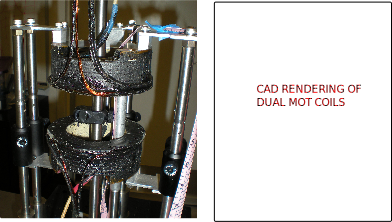
\includepdf[landscape=true]{drawings/dual_mot_coils/dual_mot_coils.pdf}

%%%%%%%%%%%%%%%%%%%%%%%%%%%%%%%%%%%%%%%%%%%%%%%%%%%%%%%%%%%%%%%%%%%
%%%%	Bibliography
%%%%%%%%%%%%%%%%%%%%%%%%%%%%%%%%%%%%%%%%%%%%%%%%%%%%%%%%%%%%%%%%%%%

%\bibliographystyle{ieeetr}
%\bibliography{bibliography}
%\addcontentsline{toc}{chapter}{Bibliography}
\printbibliography

\end{document}